\documentclass{template/abschlussarbeit}

%%%%%%%%%%%%%%%%%%%%%%%%%%%%%%%%%%%%%%%%%%%%%%%%%%%%%%%%%%%%
% Allgemeine Variablen fuer die Abschlussarbeit (mit eigenen
% Angaben ausfuellen!)
%%%%%%%%%%%%%%%%%%%%%%%%%%%%%%%%%%%%%%%%%%%%%%%%%%%%%%%%%%%%

\AutorVorname{Hutan}
\AutorNachname{Baghery Moghaddam}
\AutorGeburtsort{Leverkusen}
\AbschlussarbeitTitel{User-Level Thread-Management in Java}
% Bachelorarbeit, Projektarbeit, Masterarbeit
\AbschlussarbeitTyp{Bachelor Thesis}
% keywords durch , getrennt
\AbschlussarbeitKeywords{Distributed Systems, Big Data, Cloud}
\Ort{Düsseldorf}
\Datum{19. March 2020}
\Erstgutachter{Prof. Dr. Michael Schöttner}
\Zweitgutachter{Dr. Jens Bendisposto}

% Hier den vollstaendigen Dateinamen der bibtex Datei angeben
% Falls diese in einem Unterordner liegt, so ist dieser relativ
% zu dieser Datei (document.tex) anzugeben.
\LiteraturBibtexDatei{library.bib}

% Der Anhang (falls vorhanden) wird hier genauso wie diese
% Bibtex-Datei angegeben (jedoch ohne .tex-Endung!)
\AnhangDatei{chap/anhang}

%%%%%%%%%%%%%%%%%%%%%%%%%%%%%%%%%%%%%%%%%%%%%%%%%%%%%%%%%%%%
% Optionen/Schalter um bestimmte Abschnitte an-/auszuschalten
% WICHTIG: Nicht genutzte/leere Abschnitte vor der Abgabe/
% dem finalen Druck abschalten durch auskommentieren.
% Gleiches gilt fuer die Todo Liste, welche nicht in die 
% finale Version gehoert.
%%%%%%%%%%%%%%%%%%%%%%%%%%%%%%%%%%%%%%%%%%%%%%%%%%%%%%%%%%%%

\Titelblatt
\Inhaltsverzeichnis
\Abbildungsverzeichnis
\Anhang
\Erklaerung

%%%%%%%%%%%%%%%%%%%%%%%%%%%%%%%%%%%%%%%%%%%%%%%%%%%%%%%%%%%%

% Custom additions

\lstdefinelanguage{custom-java}
{
    language=java,
    % morecomment=[s][\color{gray}]{@}{\ },
    morekeywords={var},
}

\lstdefinelanguage{no-numbers}
{
    language=java,
    numbers=none,
}

\newcommand{\myparagraph}[1]{\paragraph{#1}\mbox{}\\}

\newcommand{\at}{\makeatletter @\makeatother}



%%%%%%%%%%%%%%%%%%%%%%%%%%%%%%%%%%%%%%%%%%%%%%%%%%%%%%%%%%%%

\begin{document}
\begin{abschlussarbeit}

    %%%%%%%%%%%%%%%%%%%%%%%%%%%%%%%%%%%%

    \chapter{Introduction}
Solaris 2.6  was released in July 1997. \cite{wiki:solaris} Before Solaris 2.6 was released Java versions on the Solaris platform used green threads.
Green threads were user-level threads, scheduled by the programmers themselves instead of relying on the operating system. Solaris was unable to process more than one green thread at a time, which resulted in a many-to-one model. Java applications were able to create as many green threads per application as they wanted to, but only one of them would be processed at a time. Therefore multithreading was impossible for Java applications on Solaris. \cite{oracle:solaris} With this big problem in mind, Sun Microsystems started to abandon green threads.
Several different solutions were used over the years depending on which platform Java was running on. Nowadays it is universally known that a Java thread corresponds to a kernel-level thread when looking at it in a very simplified matter.
\\
\\
About two decades after green threads were abandoned, project Loom is trying to bring user-level threads back into the Java ecosystem. The reason for this is the heavy weight of kernel-level threads and the growing popularity of extreme multithreading. Particularly in cloud computing resources are scarce. Project Loom is sponsored by the HotSpot Group and therefore Oracle themselves. It is part of OpenJDK's Java Virtual Machine: HotSpot. Project Loom calls their user-level threads virtual threads. \cite{loom:proposal}
\\
\\
The goals of this work are:
\begin{itemize}
    \item Examining how project Loom implements virtual threads.
    \item Comparing virtual threads to common Java threads.
    \item Giving a forecast for the future of virtual threads.
\end{itemize}
In the first chapter of this thesis, the required basics will be explained. Afterwards, the architecture of project Loom's virtual threads is analyzed. Once that is done, the virtual threads will be used in experiments in the following chapter. Finally, a conclusion is drawn.





    
\chapter{Background}

\section{Processor - Process - Thread}

\myparagraph{Processor}
The processor is the central processing unit of a computer. The processor is also called CPU for short. Each processor can execute exactly one specific instruction set. Examples for known instruction sets are the x86 architecture and the ARM architecture. A processor usually consists of several components. Among others, a processor contains the ALU (arithmetic-logical unit), the MMU (memory management unit), and several other registers. \cite{Tannenbaum:21}
\\
Nowadays processors usually have several cores. \cite{Tannenbaum:87} This means that there are several mini chips on these processors, which can execute instructions independently of each other. Furthermore, many CPUs are capable of multithreading. Multithreading allows a core to remember the state of two threads. This allows the core to switch quickly between them. This is also called pseudo-parallelism.\cite{Tannenbaum:23}
\\
If one wants to increase the performance of a processor, there are two options. Either one increases the individual performance of the cores or one increases the number of cores. Today, the performance of an individual core is close to the limit of what is physically possible. Due to limitations in heat generation, only small increases in performance are possible today. On the other hand, increasing the number of cores is far from the limit. Multi-core systems are not only in demand in the industry but are also available to private individuals. [Citation needed]
If you look at the sales figures of the german computer parts reseller Mindfactory, you can see that most of the sold processors have 4, 6, 8 and even 16 cores. 

\begin{figure}[H]
  \centering
  \begin{subfigure}[b]{1.0\textwidth}
    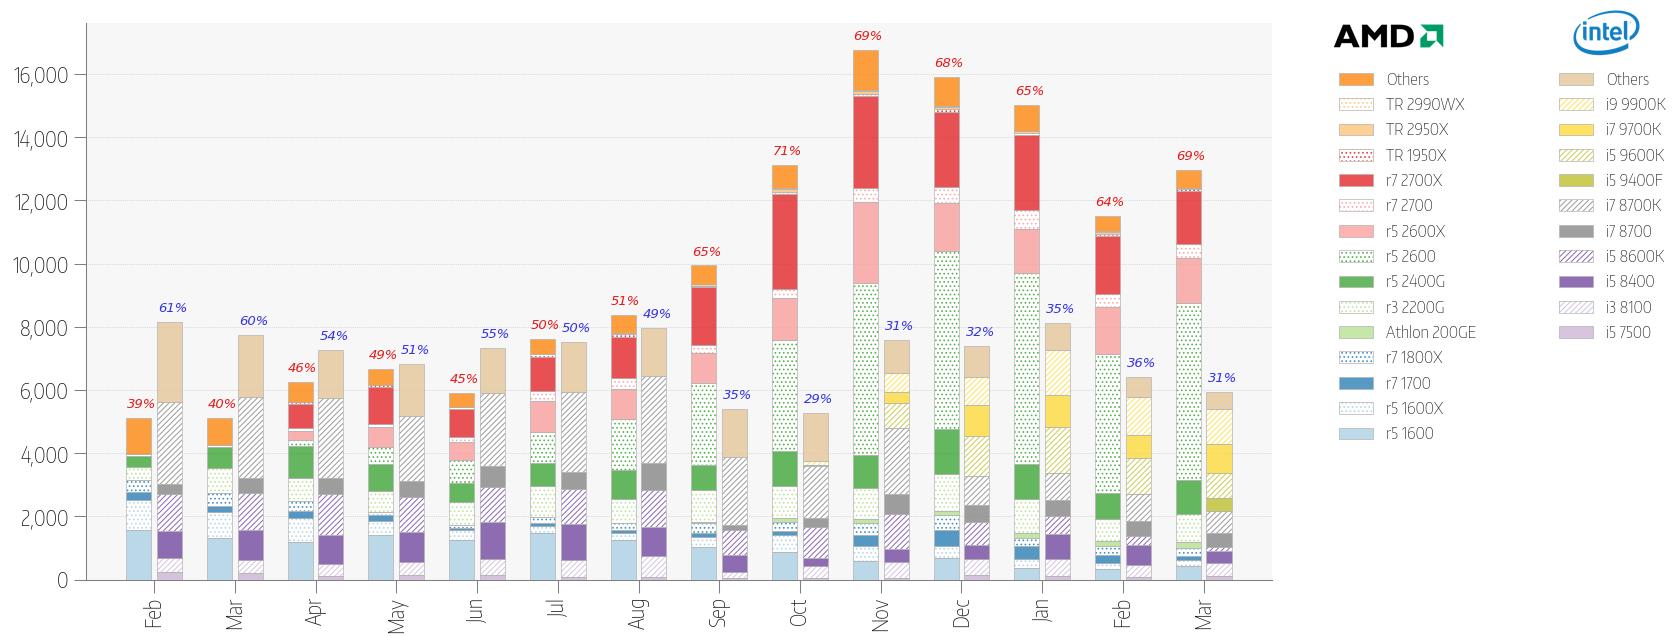
\includegraphics[width=1.0\linewidth]{img/mindfactory-sales2.png}
  \end{subfigure}
  \caption{Mindfactory CPU Sales \cite{forbes:mindfactory:sales}}
  \label{Mindfactory CPU Sales}
\end{figure}

\myparagraph{Process}
A process is a program that is being executed. In the following figure, the relation between a process and a program is presented.

\begin{figure}[H]
  \centering
  \begin{subfigure}[b]{1.0\textwidth}
    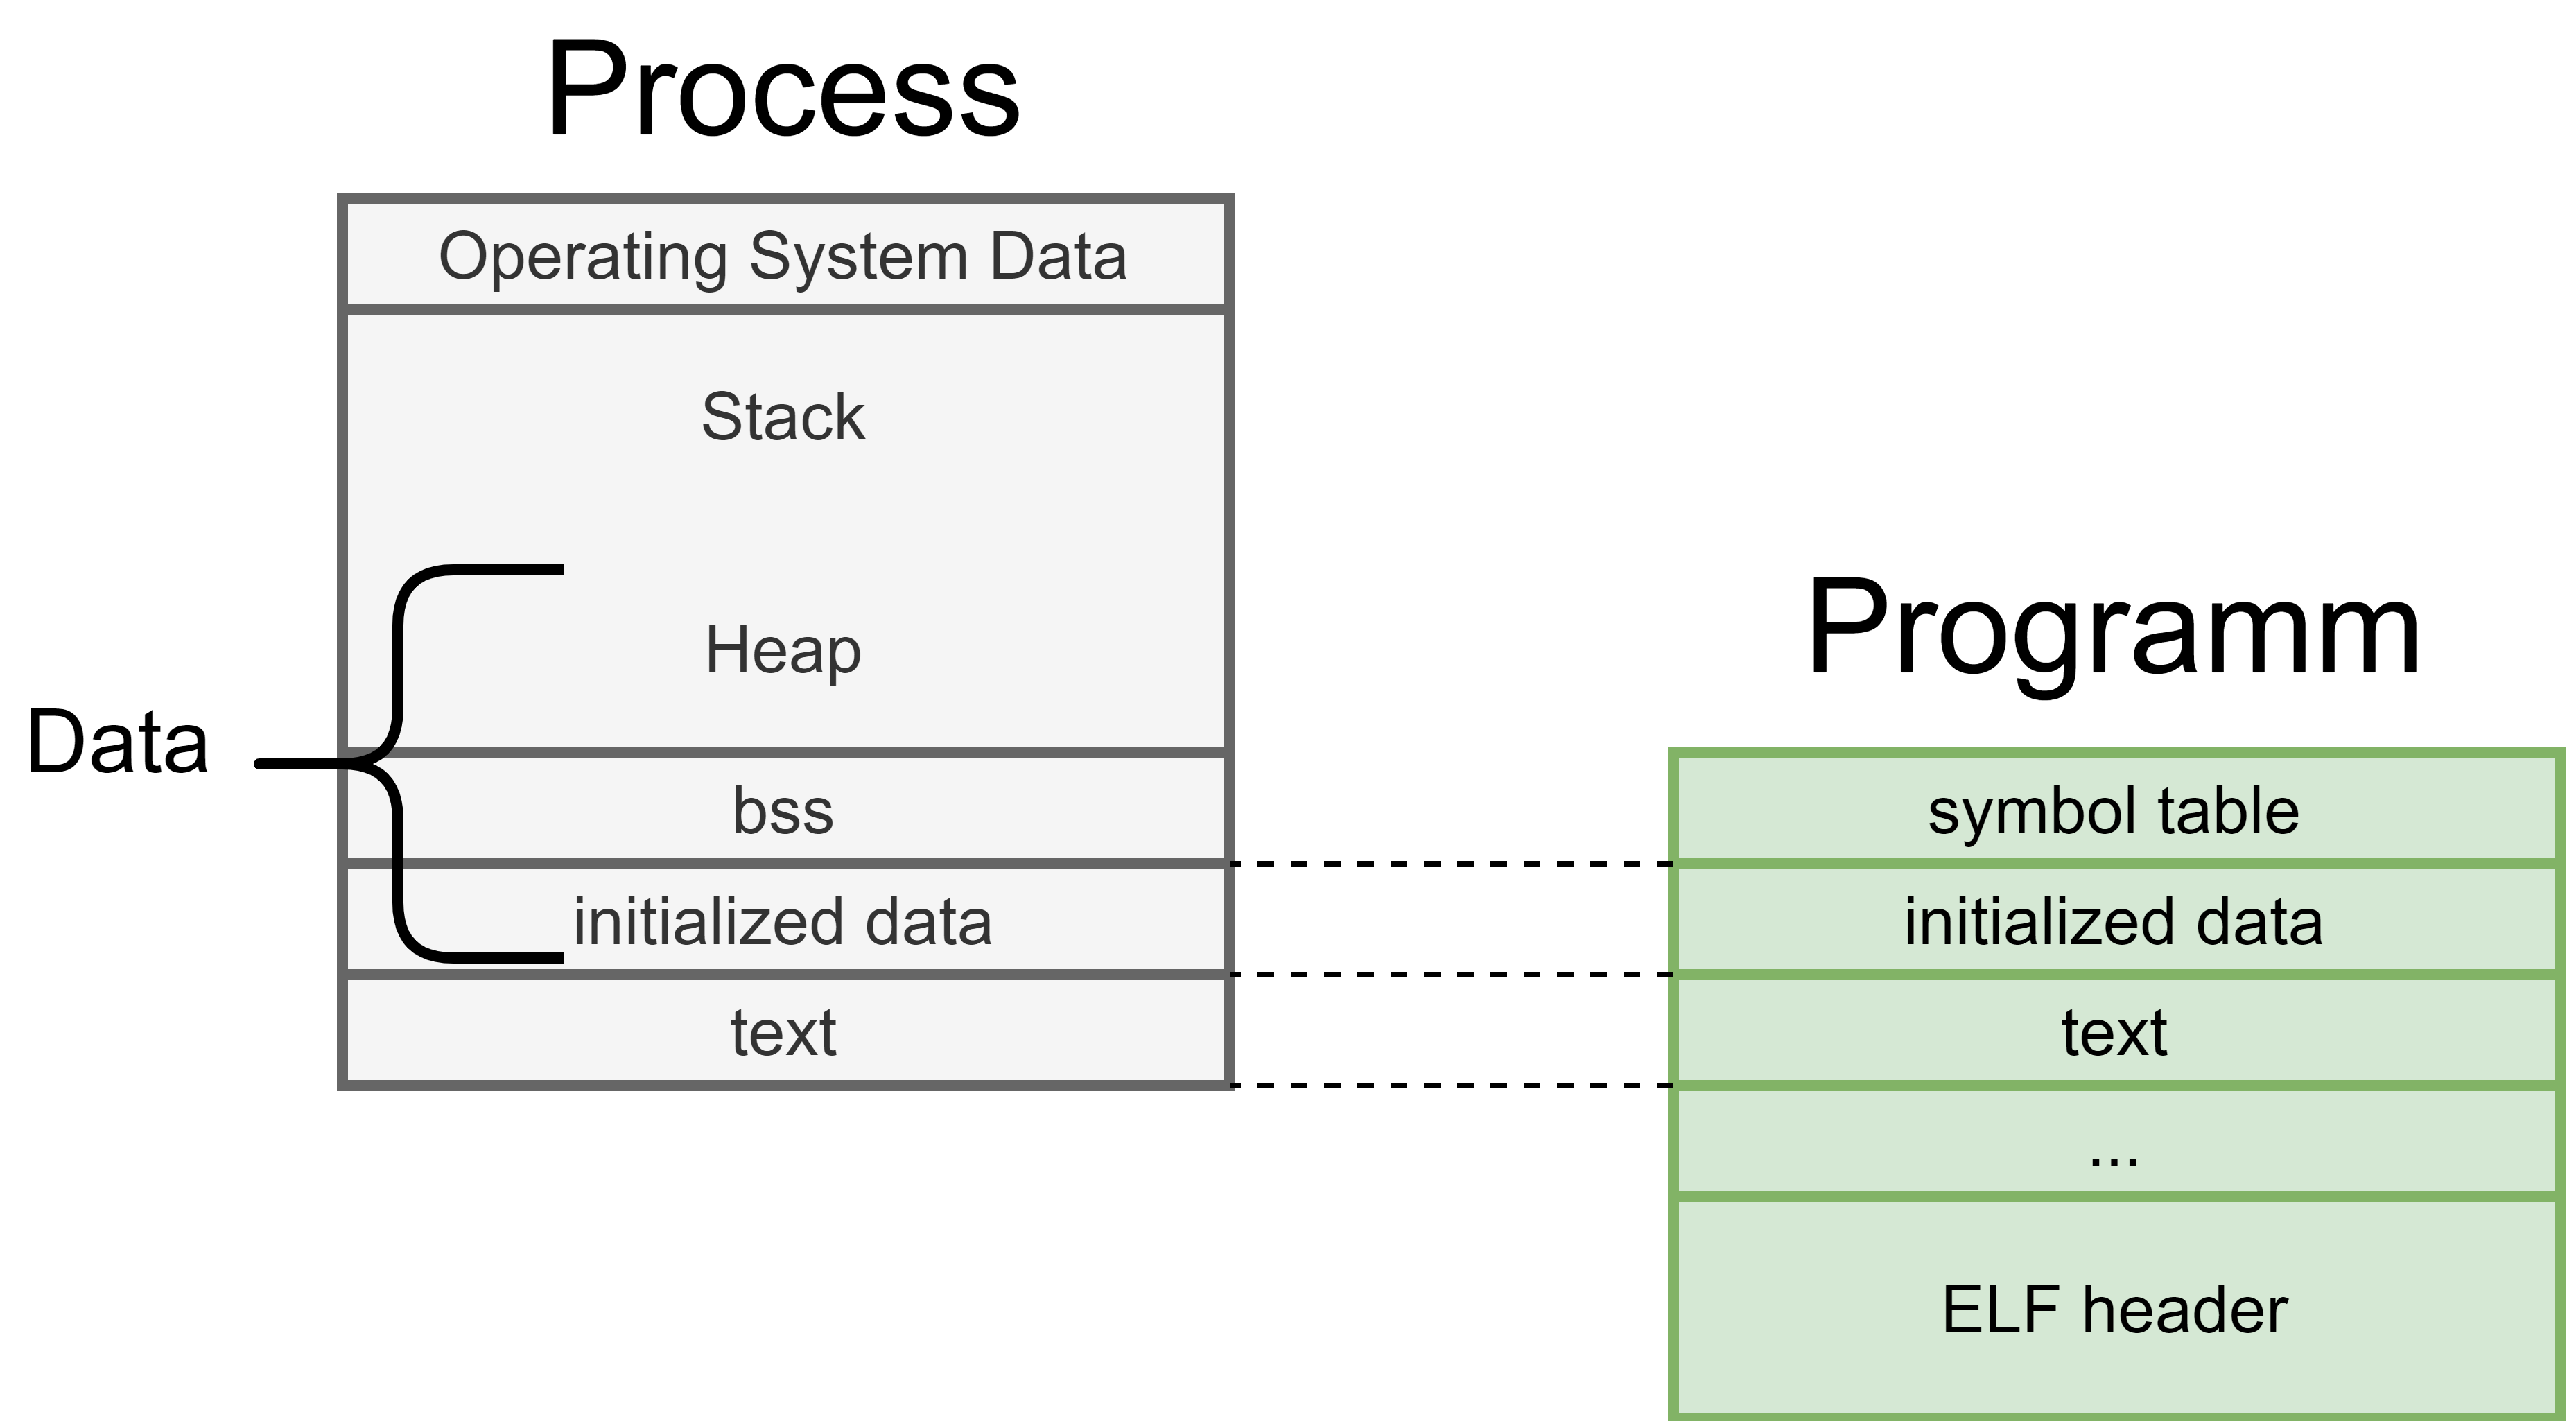
\includegraphics[width=1.0\linewidth]{img/process-program.png}
  \end{subfigure}
  \caption{Process vs Program \cite{Schoettner:bs18:4.5}}
  \label{process-program}
\end{figure}

The segment \textit{text} contains the programcode.
The segment \textit{initialized data} contains initialized global and static variables.
The segment \textit{bss} contains not yet initialized global variables and static variables.
The \textit{heap} is the extension of the \textit{bss}.
The \textit{stack} is used for saving local variables, function parameters and memory areas of register contents.
Both the \textit{stack} and the \textit{heap} will be dynamically extended if needed.\cite{Schoettner:bs18:4.5}
\\
Processes allow a system to process several programs simultaneously. An active process can have three different statuses.
\\
\begin{figure}[H]
  \centering
  \begin{subfigure}[b]{1.0\textwidth}
    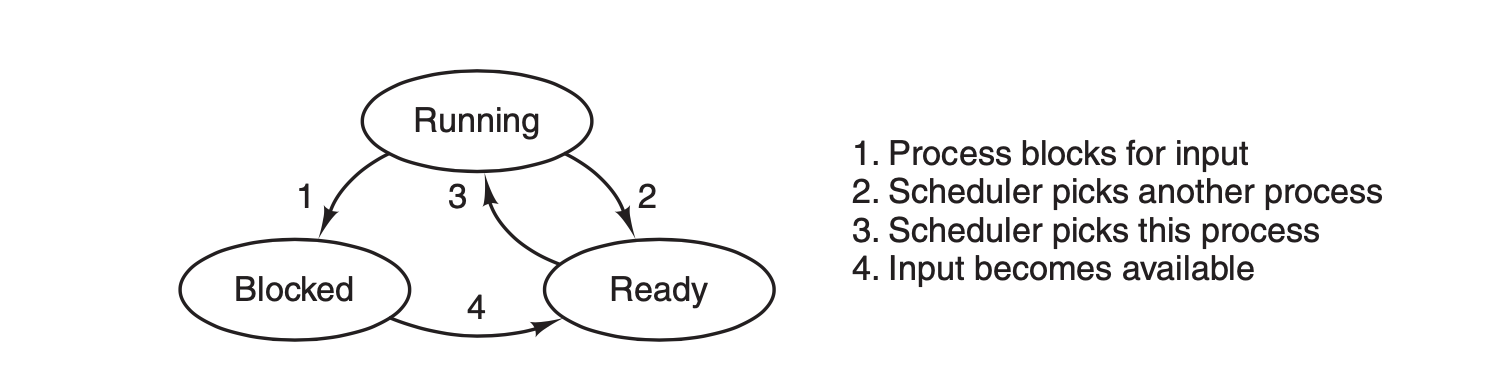
\includegraphics[width=1.0\linewidth]{img/prozess-status.png}
  \end{subfigure}
  \caption{Process Status \cite{Tannenbaum:93}}
  \label{process-status}
\end{figure}

The scheduler plays an important role here. A scheduler is responsible for when a process is processed by the CPU. In UNIX systems, for example, a round-robin scheduler is used. This changes the active process in a predetermined cycle, such as 10-100ms. \cite{Schoettner:bs18:6.6.4}
An active process is a process with the status \textit{Running}. The CPU is then assigned to the process and executes the program of the process. If the CPU is removed from the process by the scheduler, the process is in \textit{Ready} status. The process is then ready to be reassigned to the CPU and is waiting for it. A process can also block. This happens if the process has to wait for a certain input. The process is then in \textit{Blocked} status and will not change to \textit{Ready} status until the input becomes available. \cite{Tannenbaum:93}

\myparagraph{Thread}
A process is heavy. Each process has its own address space and switching between processes takes a lot of time. Therefore threads were created as lightweight processes. Threads are part of a process and therefore they share the same address space. Switching between threads is a lot faster. The following diagram lists the unique items for threads and processes.
\\
\begin{figure}[H]
  \centering
  \begin{subfigure}[b]{0.6\textwidth}
    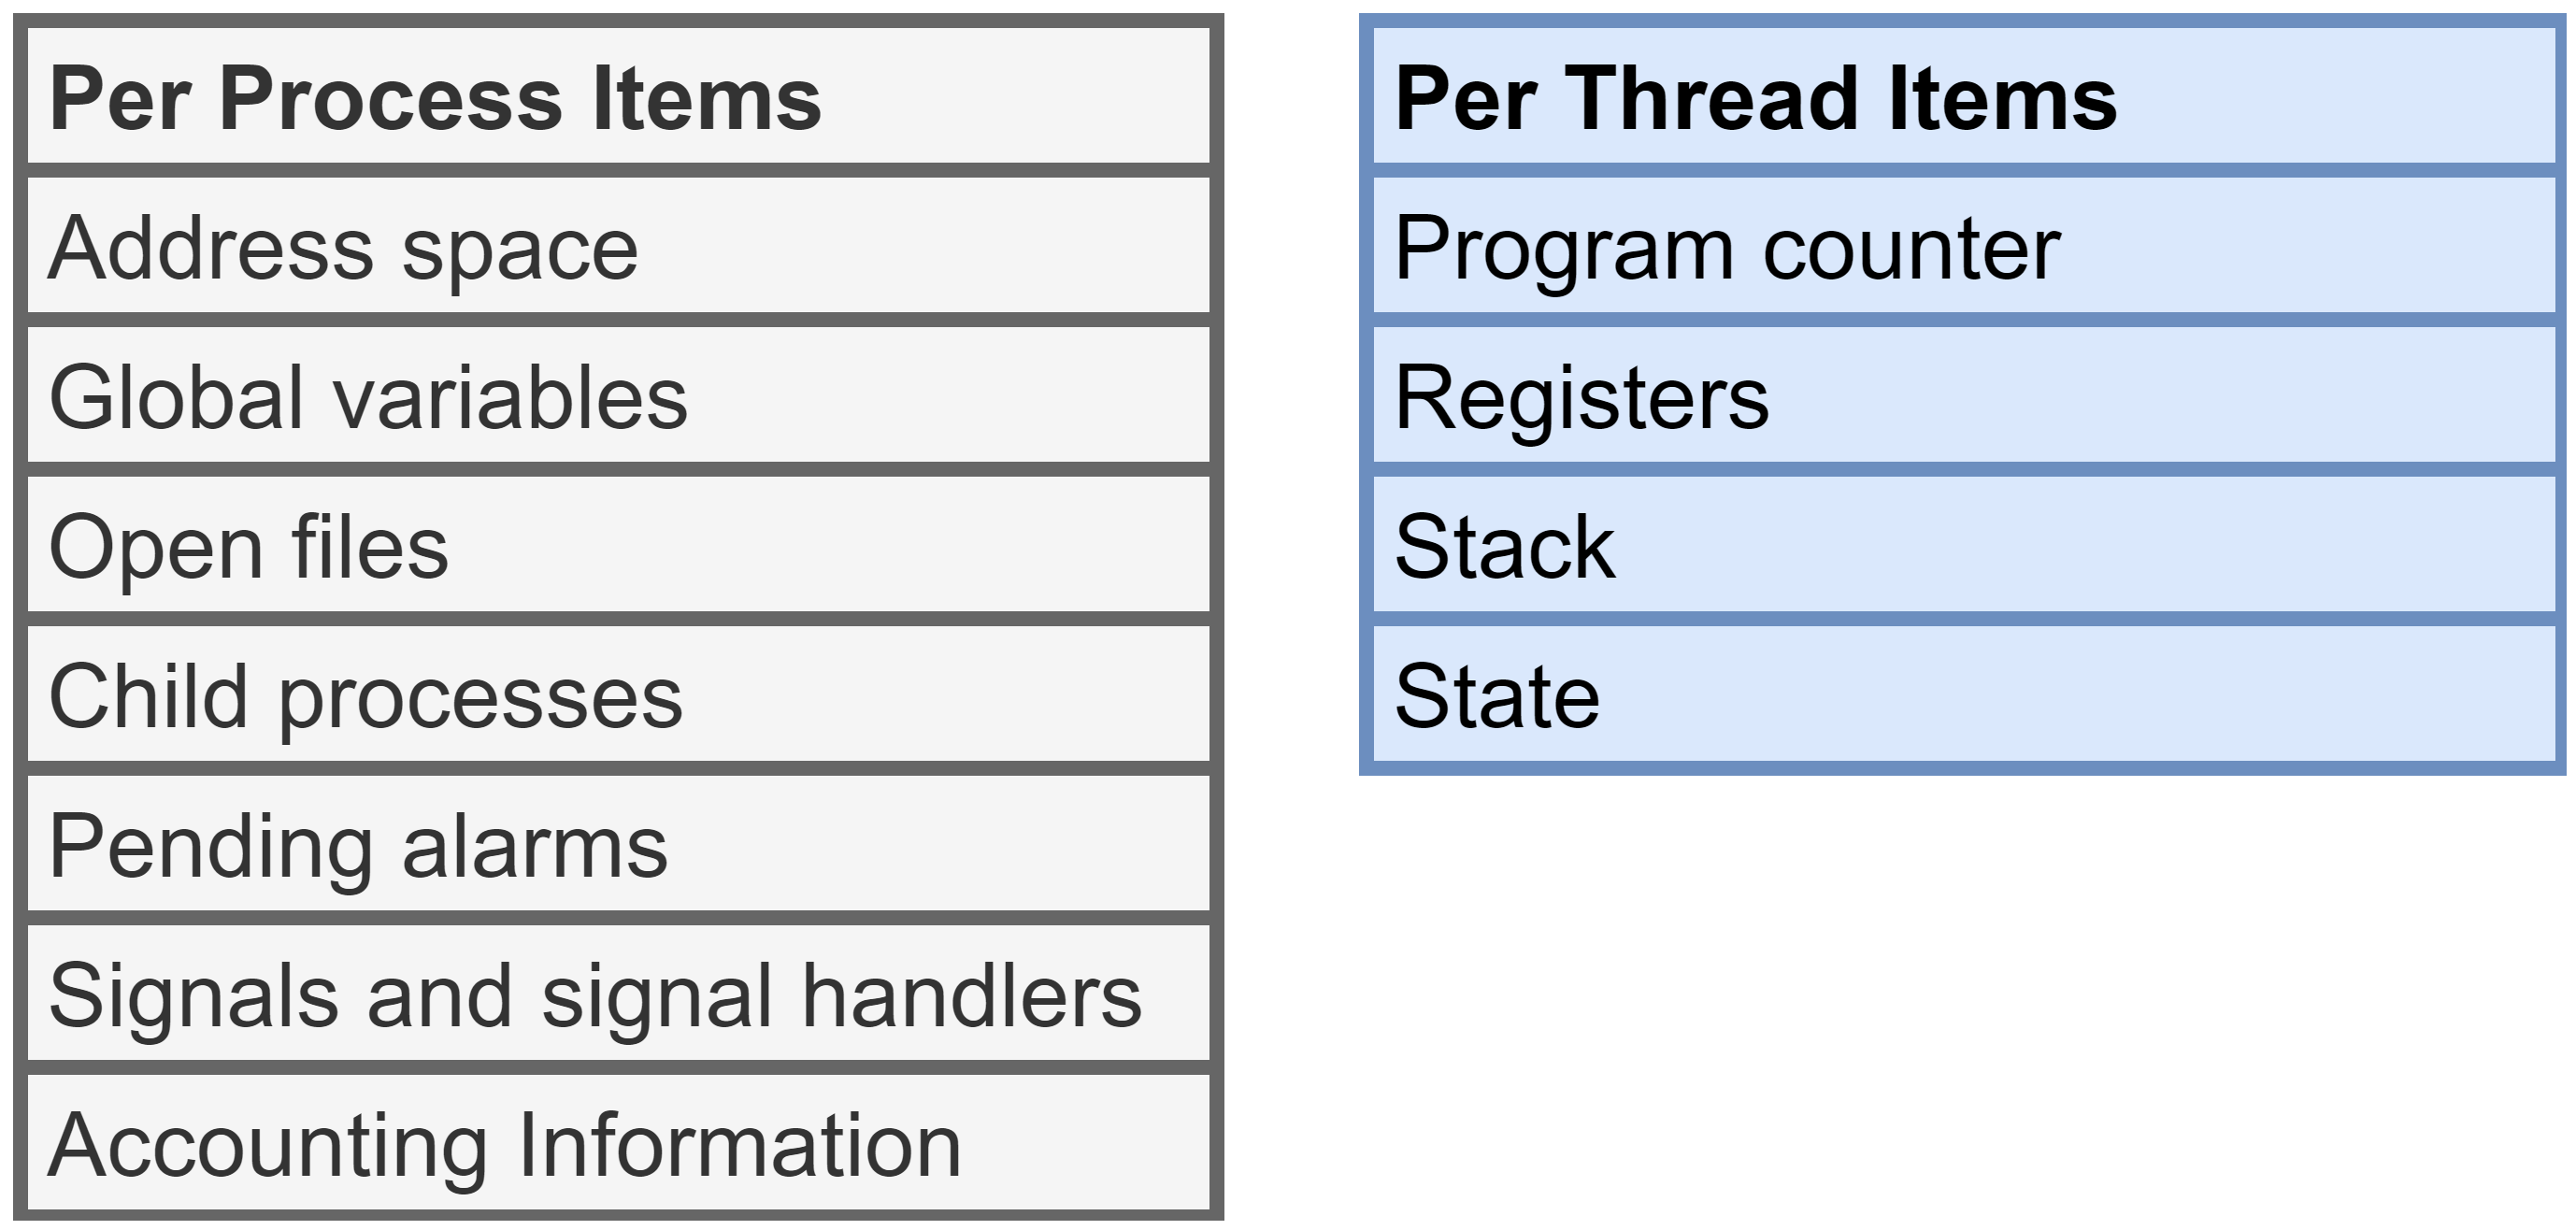
\includegraphics[width=1.0\linewidth]{img/process-thread-items.png}
  \end{subfigure}
  \caption{Process vs Thread \cite{Tannenbaum:104}}
  \label{Process vs Thread}
\end{figure}

Each process can have many threads. The following figure shows the hierarchy of processes and threads.

\begin{figure}[H]
  \centering
  \begin{subfigure}[b]{1.0\textwidth}
    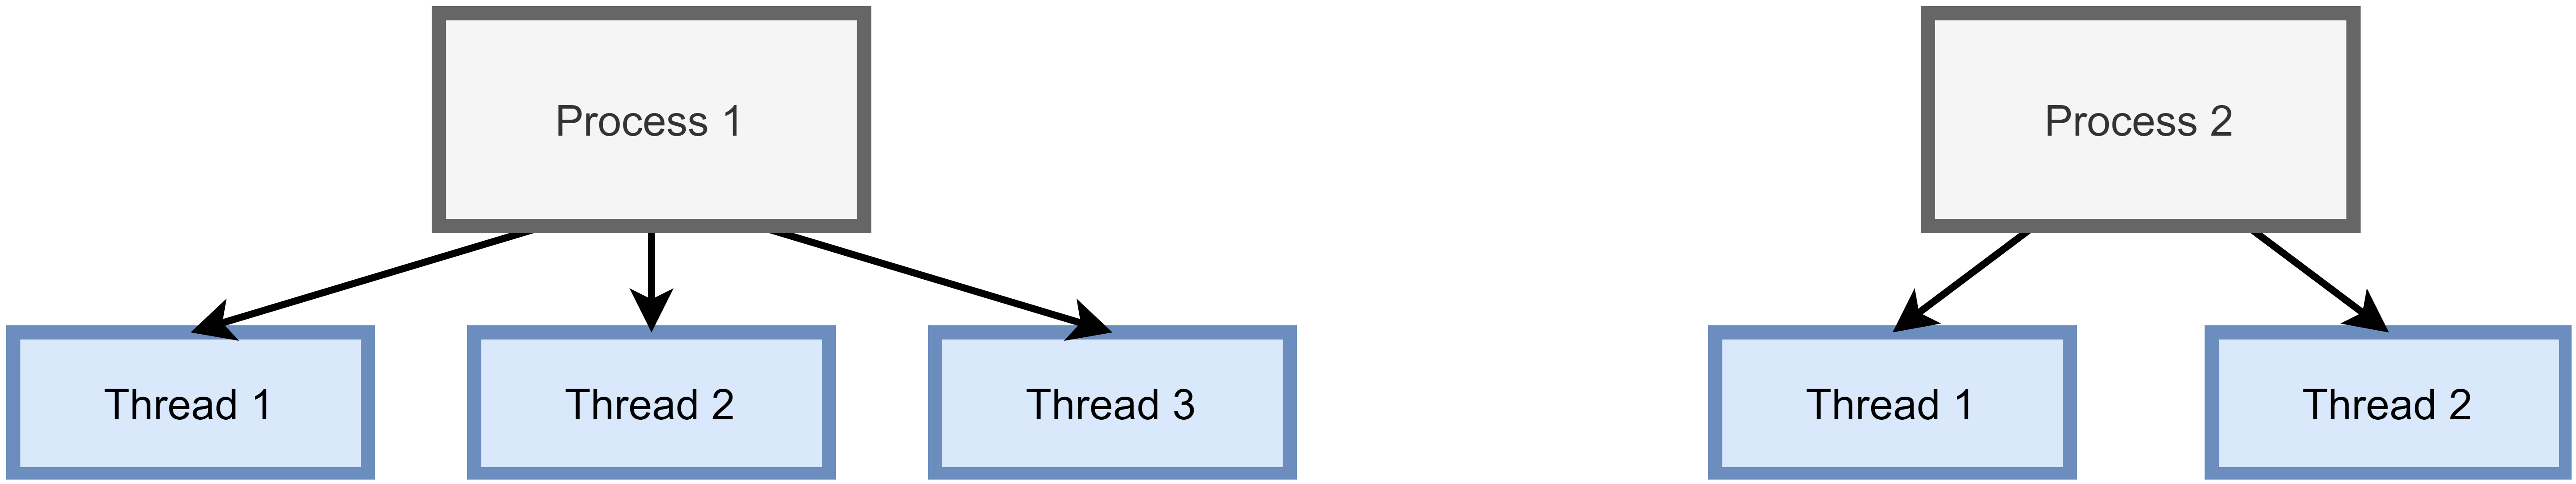
\includegraphics[width=1.0\linewidth]{img/process-thread.png}
  \end{subfigure}
  \caption{Process - Thread - Hierarchy}
  \label{Process - Thread - hierarchy}
\end{figure}
In modern programming, the line between processes and threads gets somewhat blurred, because processes often start with a single thread. Standalone processes without any threads are a thing of the past.
\\
\\
Threads increase CPU efficiency. Whenever a thread has to block, for example, because it has to wait for I/O input, another thread of the same process can quickly continue and make use of the CPU. Constantly switching between processes would be very inefficient.
\\
\\
A distinction is made between two types of threads. Kernel-level threads, which are managed directly by the operating system's scheduler and User-level threads, where the programmer has to do the scheduling himself.\cite{Schoettner:bs18:6.4}

\section{Atomic Functions}
In the context of multithreading a race condition occurs, when multiple threads utilize the same variables. Per default, the result of such a race condition is not deterministic. This is unwanted behavior. The solution is to only allow one thread to access that variable at a time. This can be realized by using a lock variable, which gets set to True whenever one thread tries to access the variable. Once the thread is done, the lock gets released by setting it to False. The immediate problem is, that another race condition occurs. Instead of having a race condition for the old variables, now one has a race condition for the lock. \cite{Schoettner:bs18:7.4}
To fix this, the lock variable has to be set atomically. "An operation acting on shared memory is atomic if it completes in a single step relative to other threads." \cite{Preshing}
\\
\\
In Java, there are multiple implementations of atomic functions. One of them is the VarHandle class. A VarHandle is a reference to a variable. VarHandles support multiple access modes with different functions. In this context, the most important functions are part of the atomic update access modes. An example of such a function would be:
\begin{lstlisting}[language=custom-java]
  public final boolean compareAndSet(Object... args)
\end{lstlisting}
compareAndSet receives two parameters: expectedValue and newValue. It will check whether the current value equals the expectedValue. If that is the case it will set the value to newValue and return True. If not, the value remains unchanged and False is returned.

\section{Intrinsic Functions}
"In compiler theory, an intrinsic function is a function available for use in a given programming language whose implementation is handled specially by the compiler. Typically, it substitutes a sequence of automatically generated instructions for the original function call." \cite{wiki:intrinsics}
\\
\\
OpenJDK provides a descriptive example, using the String::format function. Consider the following code:
\begin{lstlisting}[language=custom-java]
  String name = ...
  int age = ...
  String s = String.format("%s: %d", name, age);
\end{lstlisting}
Without intrinsification this piece of code would be translated to inefficient bytecode.
Using the knowledge that the format specifier is constant, a more efficient translation to bytecode is possible. According to OpenJDK, the more efficient bytecode runs 30-50 times faster than the first one. \cite{OpenJDK:intrinsics}
\\
\\
Intrinsic functions are often abbreviated as intrinsics.


\subsection{C/C++}
There are many different C and C++ compilers. As an example Microsoft's compiler supports intrinsics. In Microsoft's implementation, "if a function is an intrinsic, the code for that function is usually inserted inline, avoiding the overhead of a function call and allowing highly efficient machine instructions to be emitted for that function. An intrinsic is often faster than the equivalent inline assembly, because the optimizer has a built-in knowledge of how many intrinsics behave, so some optimizations can be available that are not available when inline assembly is used. Also, the optimizer can expand the intrinsic differently, align buffers differently, or make other adjustments depending on the context and arguments of the call." \cite{Microsoft:intrinsics}
\\
\\
Therefore intrinsics are a powerful tool to increase performance, even in low-level languages, which support inline assembly.


\subsection{Java}
Nowadays there are many different JVMs. Whether they support intrinsics or not, depends on the implementation. The JVM relevant to this thesis is HotSpot.
The HotSpot JVM supports intrinsics. The \lstinline[basicstyle=\ttfamily\color{orange}]{@HotSpotIntrinsicCandidate} annotation is used to tell the HotSpot compiler that it should check, whether an intrinsic version of the function exists. If there is an intrinsic version, the program will use that version instead of running the Java method. Since Java is supposed to be a cross-platform language, intrinsic functions have to be created individually for each platform.
For example the functions of the x86 platform are generated in src/hotspot/cpu/x86/stubGenerator\_x86\_64.cpp.
All intrinsic functions are listed in src/hotspot/share/classfile/vmSymbols.cpp.
\cite{Mok:intrinsics}

\section{Structured Concurrency}
Structured concurrency is a programming paradigm. The core idea is that whenever a task splits up into multiple subtasks, the original task will only continue once the sub-tasks are done.

\begin{figure}[H]
  \centering
  \begin{subfigure}[b]{0.4\textwidth}
    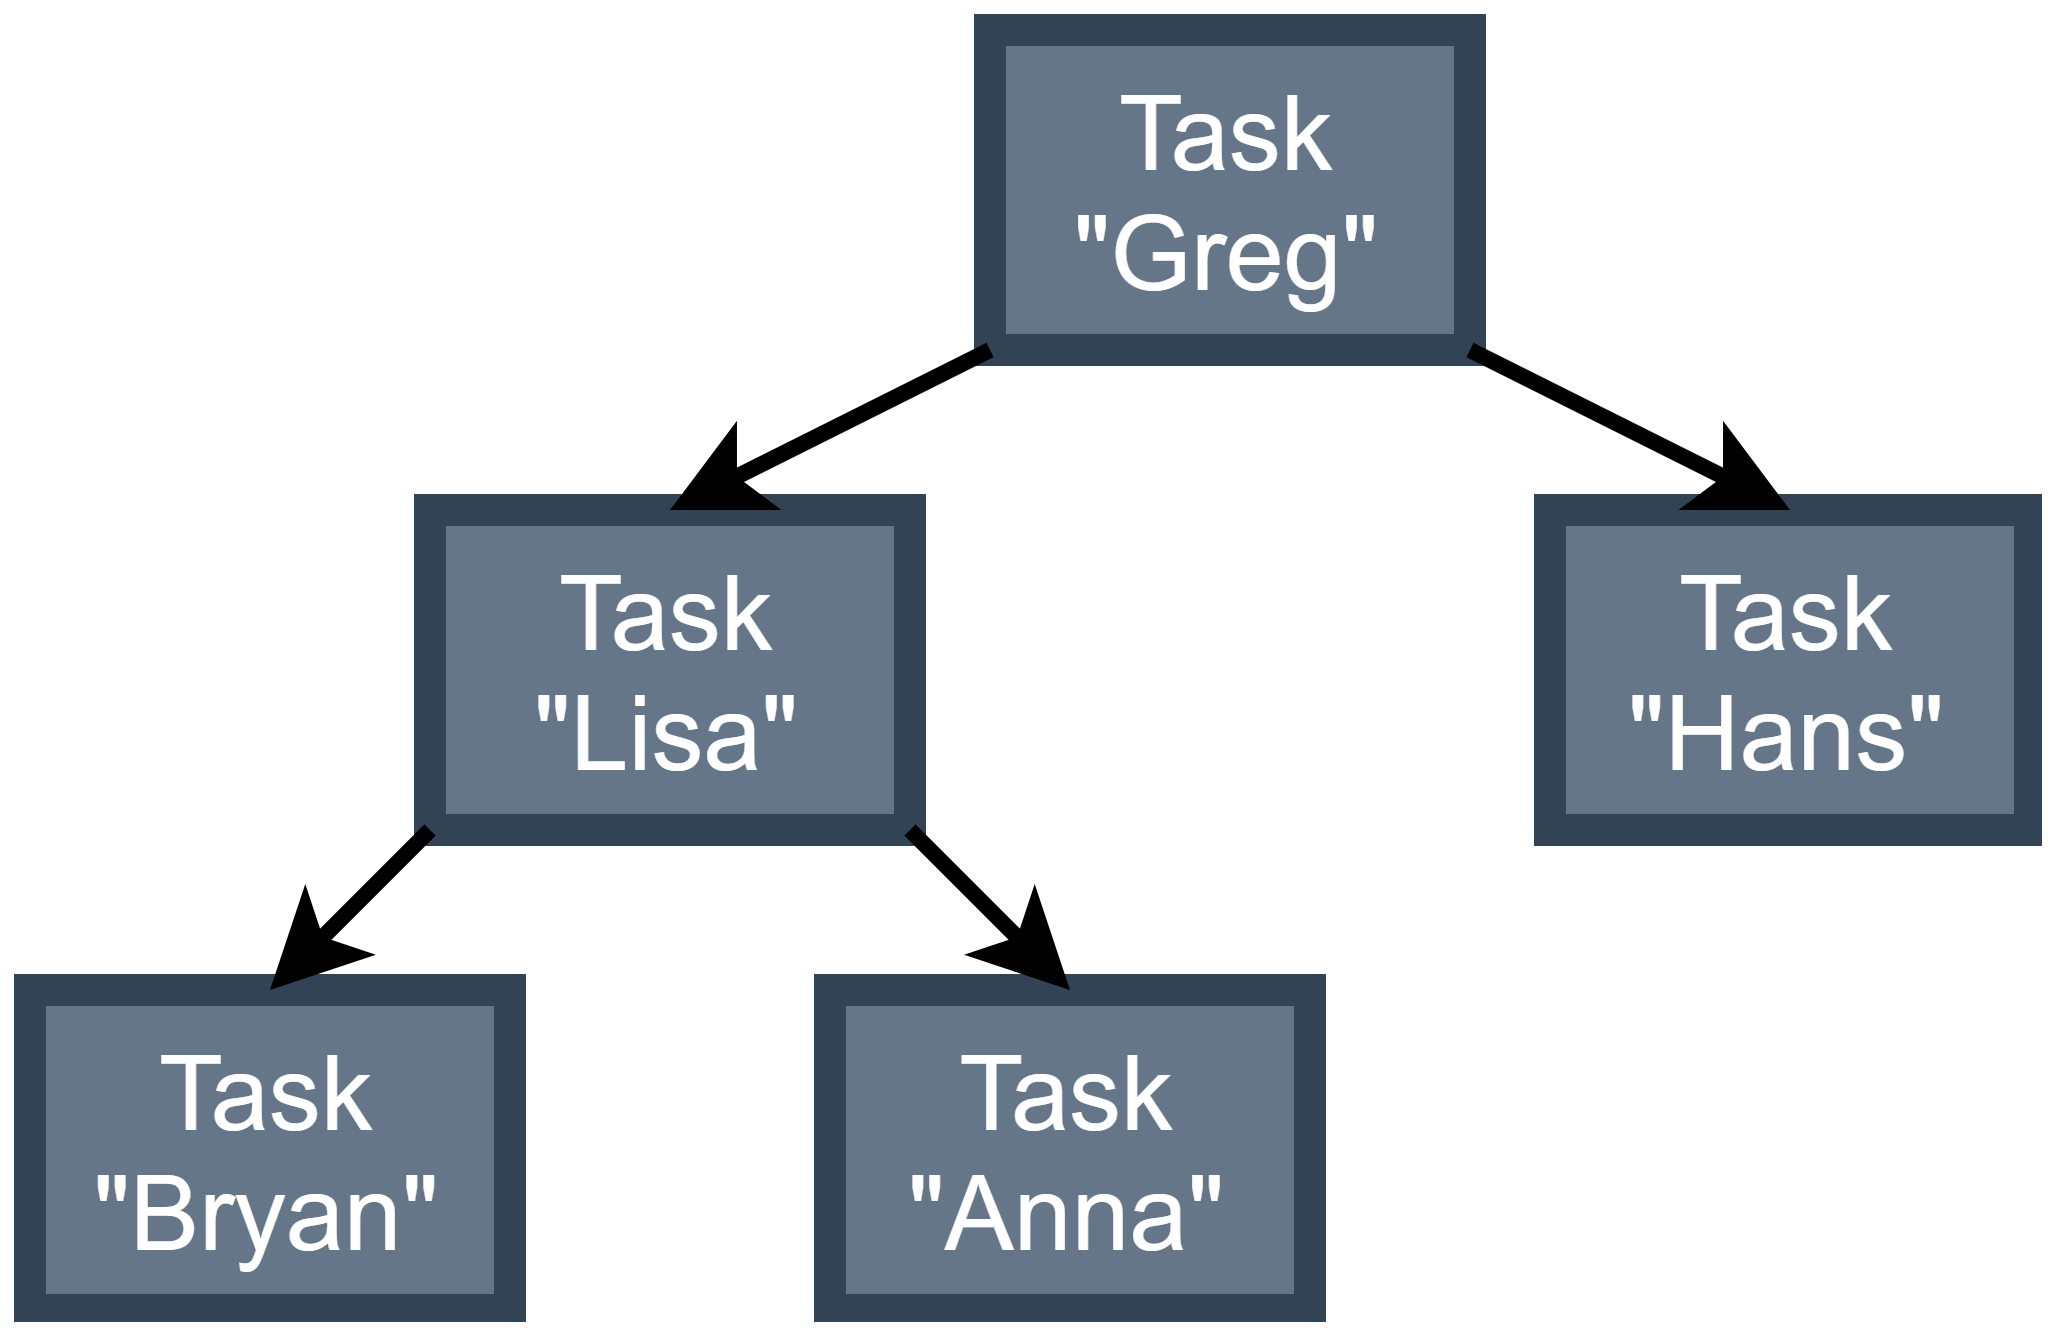
\includegraphics[width=1.0\linewidth]{img/structured-concurrency.png}
  \end{subfigure}
  \caption{Structured Concurrency}
  \label{Structured Concurrency}
\end{figure}
In this example, the main task called Greg will only continue once their sub-tasks Lisa and Hans are finished. Similar to that Lisa will only continue once Bryan and Anna are finished.
This structure can be nested as many times as necessary. Also, the main task can split into way more sub-tasks than in the example.
\\
Using structured concurrency makes the code-flow reliable and clear. This improves developing time. In order to implement structured concurrency a programming language needs to support several features, the most obvious being:
\begin{itemize}
  \item Tasks need to be able to spawn sub-tasks. There has to be a clear parent-child structure.
  \item Tasks need to be able to communicate whether they are done.
\end{itemize}

\cite{wiki:structured-concurrency}
\cite{loom:structured-concurrency}


\section{Code-Excerpts}
Project Loom is still under development. Therefore the code is still rough around the edges. Whenever code-excerpts are used in this thesis, they will be slightly altered:
\begin{itemize}
  \item Comments will be altered or removed for a better understanding of the reader.
  \item Any print outs used for debugging will be removed for the sake of clarity.
  \item Some parts of the code are experimental and exclusively used to monitor performance. Since they don't alter the actual way the program currently works, they are also removed for the sake of clarity.
  \item Correctness of any code in the JDK is extremely important. Even functions, that appear to be simple at first glance, have to be examined thoroughly. As an example, the rocket Ariane V crashed, because an Integer, which was supposed to be 64-Bit big, was saved as a 16-Bit one. The 16-Bit Integer did not have enough space to represent the Value of the variable correctly, which resulted in a crash.\cite{Ariane5} Therefore during development plenty of asserts are used to assure the correctness of the code. For example in the following code-excerpt the assert is used to assure, that the semaphore of a critical section never ends up being negative:

        \begin{lstlisting}[language=custom-java]
    public static void pin() {
      Continuation cont = currentCarrierThread().getContinuation();
      if (cont != null) {
          assert cont.cs >= 0;
          if (cont.cs == Short.MAX_VALUE)
              throw new IllegalStateException("Too many pins");
          cont.cs++;
      }
    }
    \end{lstlisting}

        Those asserts are also removed.
\end{itemize}

\section{Namechange}
Originally virtual threads were called fibers. In November 2019 project Loom decided to rename fibers to virtual threads. This decision was made due to multiple reasons:
\begin{itemize}
  \item First and foremost the name fiber made people think, that it is a new concept they would have to learn. This contradicts project Loom's core idea. The transition from kernel threads to virtual threads is envisioned to be an effortless process, which doesn't require relearning threads at all.
  \item Another reason is that the term fiber is connected to "superficially-similar-yet-essentially-different concepts"\cite{loom:namechange} elsewhere. 
\end{itemize}

\section{Java Profiler}
A Java profiler is a tool to monitor and analyze many components of a JVM during the execution of a program. As an example, it can monitor garbage collection and heap usage. There are many more things a Java profiler can monitor. Which values are monitored depends on the profiler one uses.
\subsection{VisualVM}
VisualVM is a clearly arranged Java profiler by Oracle. It is very easy to use and provides all the basic necessities. One can monitor heap size, heap usage and threads in detail. Unfortunately, VisualVM does not natively support exporting the collected data. Therefore plotting data collected with VisualVM oneself is not possible. \cite{Profiler:VisualVM}

\subsection{JProfiler}
JProfiler is another Java profiler by ej-technologies. It is much more powerful than VisualVM and allows the user to customize a lot of settings. The additional settings are of minor relevance to this thesis. The one feature that makes JProfiler a more attractive choice compared to VisualVM is the ability to export recorded data to a csv file. When only using the basic features, VisualVM and JProfiler look fairly similar on the surface. \cite{Profiler:JProfiler}
\begin{figure}[H]
  \centering
  \begin{subfigure}[b]{0.45\textwidth}
    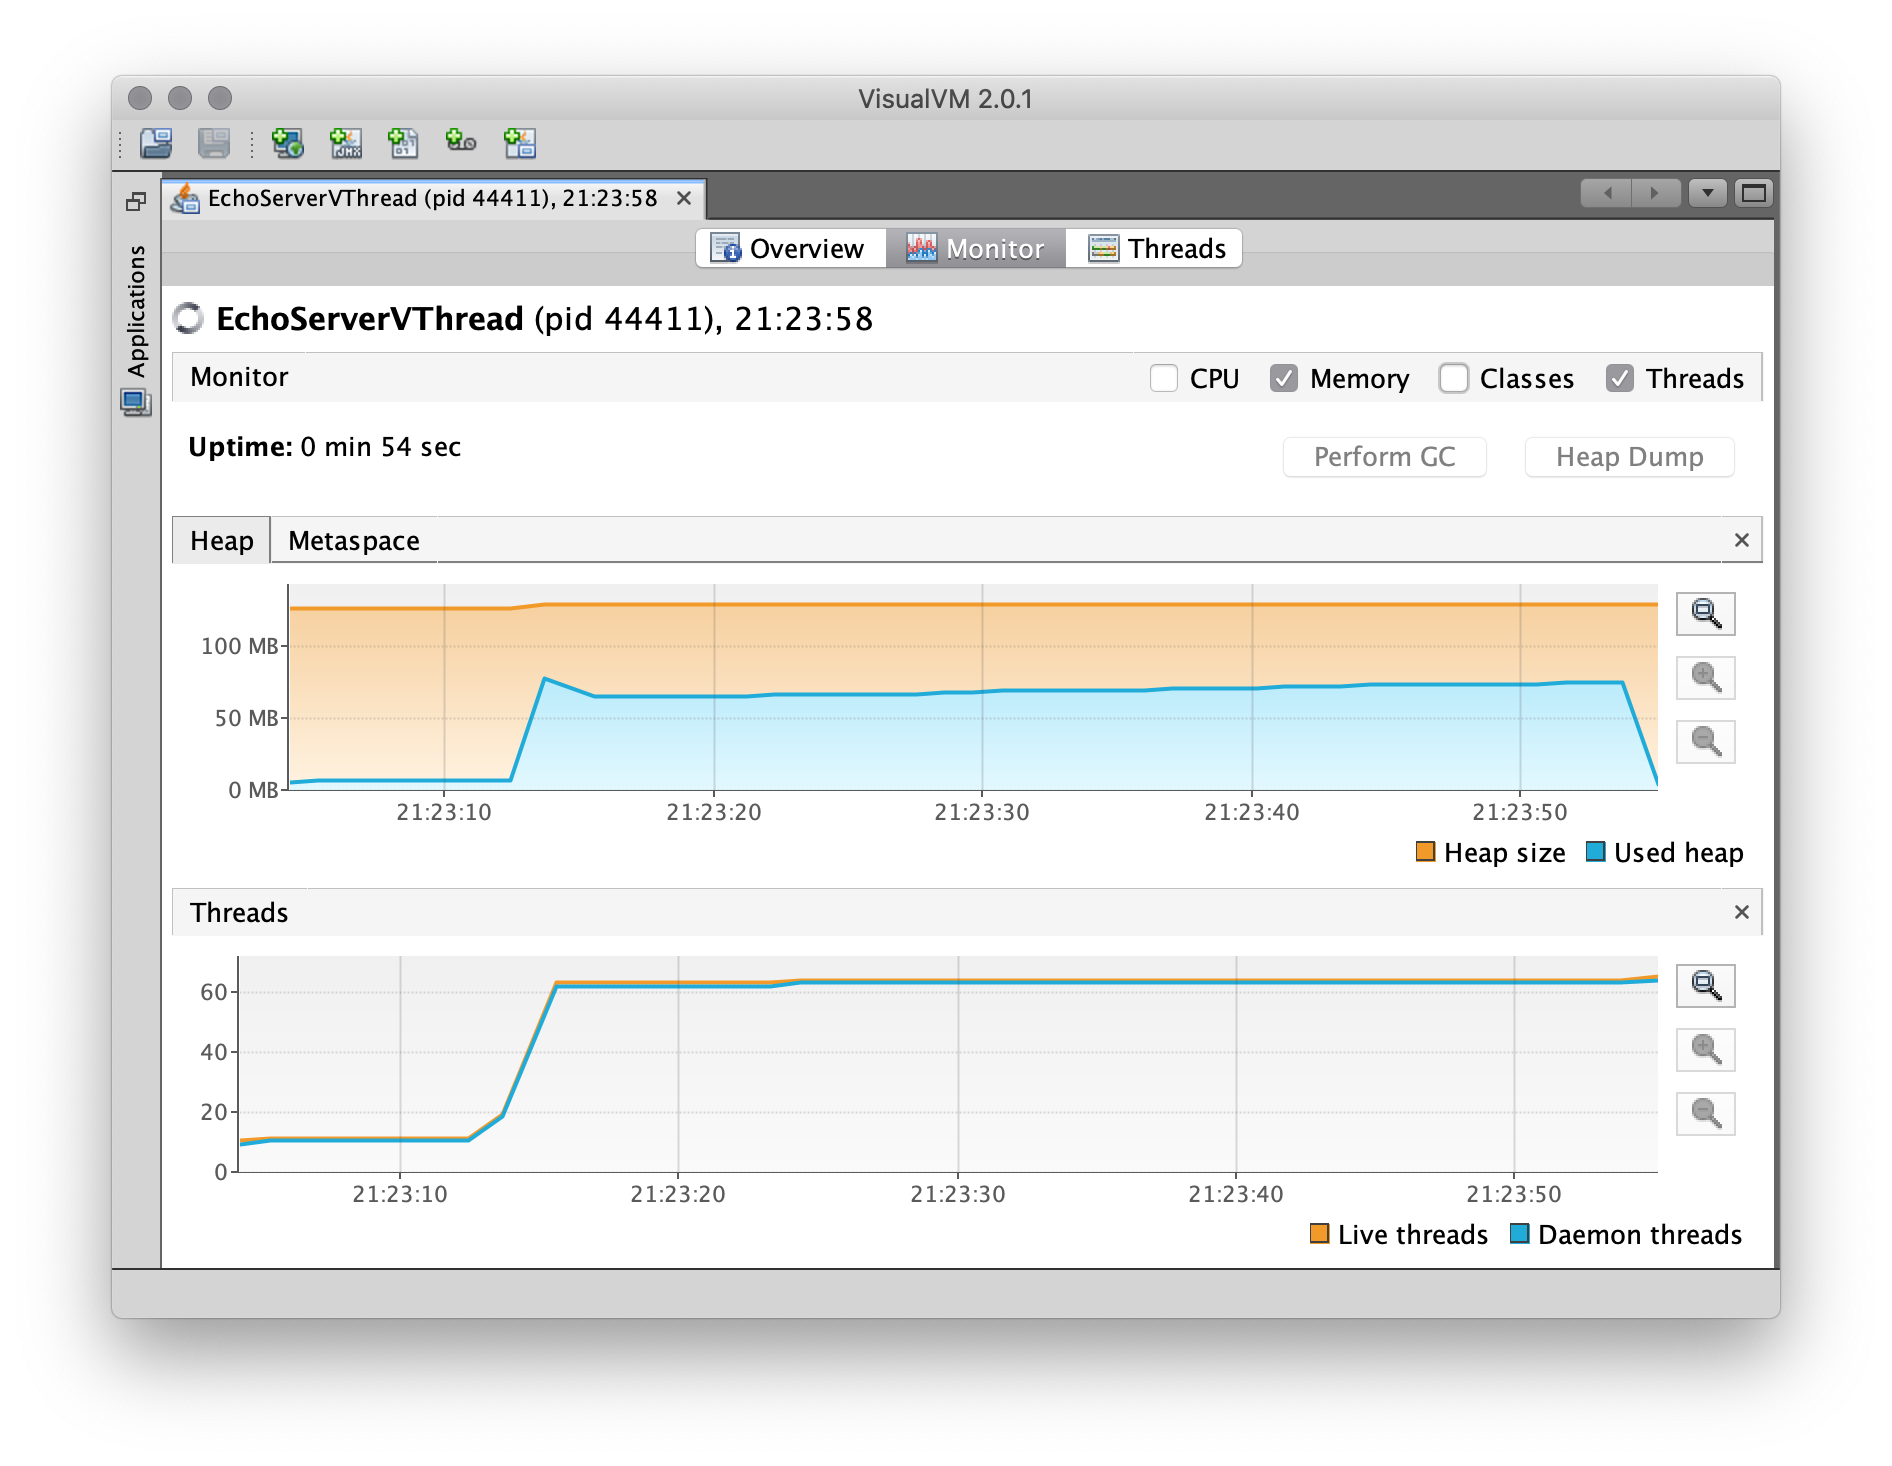
\includegraphics[width=1.0\linewidth]{img/visualvm-overview.png}
  \end{subfigure}
  \begin{subfigure}[b]{0.45\textwidth}
    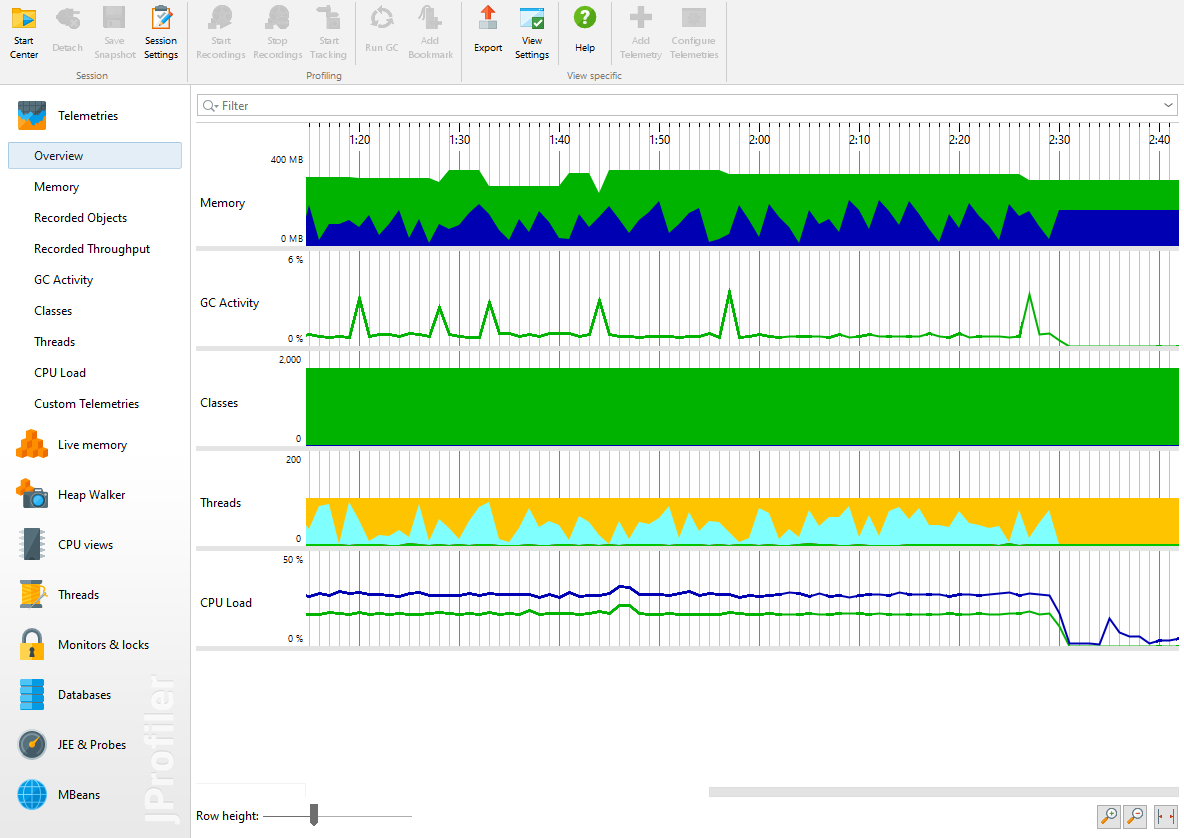
\includegraphics[width=1.0\linewidth]{img/jprofiler-overview.png}
  \end{subfigure}
  \caption{VisualVM - JProfiler - Side by side}
\end{figure}

\section{ApacheBench}
ApacheBench is a command-line utility part of the Apache HTTP Server Project, which is often abbreviated as Apache httpd. ApacheBench makes it possible to send many requests to a server to measure the time it takes to respond. It was originally designed to measure the performance of Apache servers, but it supports any other server just fine. It is very customizable. The flags most important to this thesis are used in the following example:
\begin{lstlisting}[language=no-numbers]
ab -n 1000 -c 10 -k http://localhost:5566/ 
\end{lstlisting}
This command will send 1000 requests to the server http://localhost:5566/. It will do so with a concurrency of 10. That means that 10 requests will be sent at a time. The -k flag enables the HTTP KeepAlive feature. Without it, every single request would start a new HTTP session. \cite{Apache:Bench}


\section{Java Microbenchmark Harness}
The Java Microbenchmark Harness is often abbreviated as JMH. It is a project of OpenJDK. They created it to benchmark JVMs. JVMs automatically make many optimizations to code. In general, this is very helpful, since it increases the performance. Unfortunately, it is not possible to turn off such optimizations. Therefore benchmarking Java programs is not an easy task.
\\
Benchmarks can be configured by using annotations. The most important annotations for this thesis are:
\begin{itemize}
  \item @BenchmarkMode
  \item @OutputTimeUnit
  \item @State
  \item @Warmup
  \item @Measurement
  \item @Fork
\end{itemize}
@BenchmarkMode defines what is measured. An example of that would be average time or throughput. @OutputTimeUnit defines how the measured results are returned. It can be any time unit, such as nanoseconds, seconds or minutes. Classes marked with the @State annotation are "instantiated on demand and will be reused during the entire benchmark trial" \cite{OpenJDK:jmh:3}. This annotation is a bit more complex, but most of the time it is used in a very simple manner: Just the benchmark class itself will be annotated with it. Then the JMH can reference its own fields just like any other Java program. This is called the default state. \cite{OpenJDK:jmh:4}
Typically the JVM is running a couple of Warmup runs before starting the actual benchmark. This is to be configured using the @Warmup annotation. Very similar to that the @Measurement annotation is used to configure the actual benchmark runs. Both support arguments like iterations. Which will tell the JMH how often to warmup or measure. There are two Fork options:
\begin{itemize}
  \item @Fork(0) = forking disabled
  \item @Fork(1) = forking enabled
\end{itemize}
Per default, JMH forking is enabled. Forking means that the tests will run in separate processes. This is done to avoid JVM optimizations. Often @Fork(1) is still annotated regardless, just for the sake of clarity. \cite{OpenJDK:jmh:12}
\\
\\
The OpenJDK JMH website provides information on building the projects. Any further explanation on how to use the JMH and its annotations is only provided in 38 sample Java files and the comments inside them. \cite{OpenJDK:jmh}

\section{Miscellaneous}
Project Loom is a big project with many people working on it daily. Therefore there are plenty of commits happening every single day. During this thesis, many different commits were analyzed. The code relevant to this thesis was mostly unchanged or was just slightly changed during writing it. The last commit used to analyze the code was committed on the 19.03.2020. The short hash-code for it is: 472bacfb77b
\\
\\
The code used in this thesis was run on all three major operating systems: Windows, macOS, Linux (Ubuntu 18.04 LTS in particular). The JDK used to compile and run is the same for all three: Build 15-loom+4-55, released on 22.02.2020.
\\
\\
All experiments in this thesis were run on the following environment:
\\
CPU: Intel i7 8700k
\\
RAM: 16GB
\\
OS: Ubuntu Desktop 18.04 LTS
\\
The JVM is always invoked without any additional flags.


    \chapter{Architecture of lightweight Threads in Java}

\section{Continuation}

A continuation is a sequence of instructions, that can be yielded and continued. The following example shows how a continuation can calculate the sum of the first five natural numbers while yielding after each increment.

\begin{lstlisting}[language=custom-java]
    var scope = new ContinuationScope("ContinuationScope");
    var continuation = new Continuation(scope, () ->  {
        int n = 0;
        for(int i = 0; i < 6; i++) {
            n = n + i;
            System.out.println("i: " + i + "\t" + "n: " + n);
            Continuation.yield(scope);
        }
    });

    while(!continuation.isDone()) {
        System.out.println();
        continuation.run();
    }
\end{lstlisting}

A continuation requires two arguments: A scope and a runnable. First, a scope is created. Then the continuation is created. Afterwards, the continuation is repeatedly run in a loop until it is done.
\\
\\
The scope is used to allow continuations to be nested. Each continuation has exactly one parent continuation and exactly one child continuation. Continuations run on top of kernel-level Java threads, which are referred to as carrier-threads. Every Java carrier-thread has exactly one continuation as one of its attributes. This continuation is supposed to be the innermost one.

\subsection{Stack}
Each continuation has two stacks: One for objects and one for non-objects. Project Loom calls the continuation stack horizontal stack and the thread stack vertical stack. The abbreviated versions are called h-stack and v-stack.
When a continuation yields, it will be unmounted. Unmounting copies the continuation frames from the thread stack to the continuation stack. Afterwards, the continuation frames are removed from the thread stack. Project Loom calls this process freezing.
When a continuation starts or continues, it will be mounted. Mounting is the reverse process of unmounting. Therefore project Loom calls this process thawing. \cite{OpenJDK:wiki}

\begin{figure}[h]
    \centering
    \begin{subfigure}[b]{1.0\textwidth}
        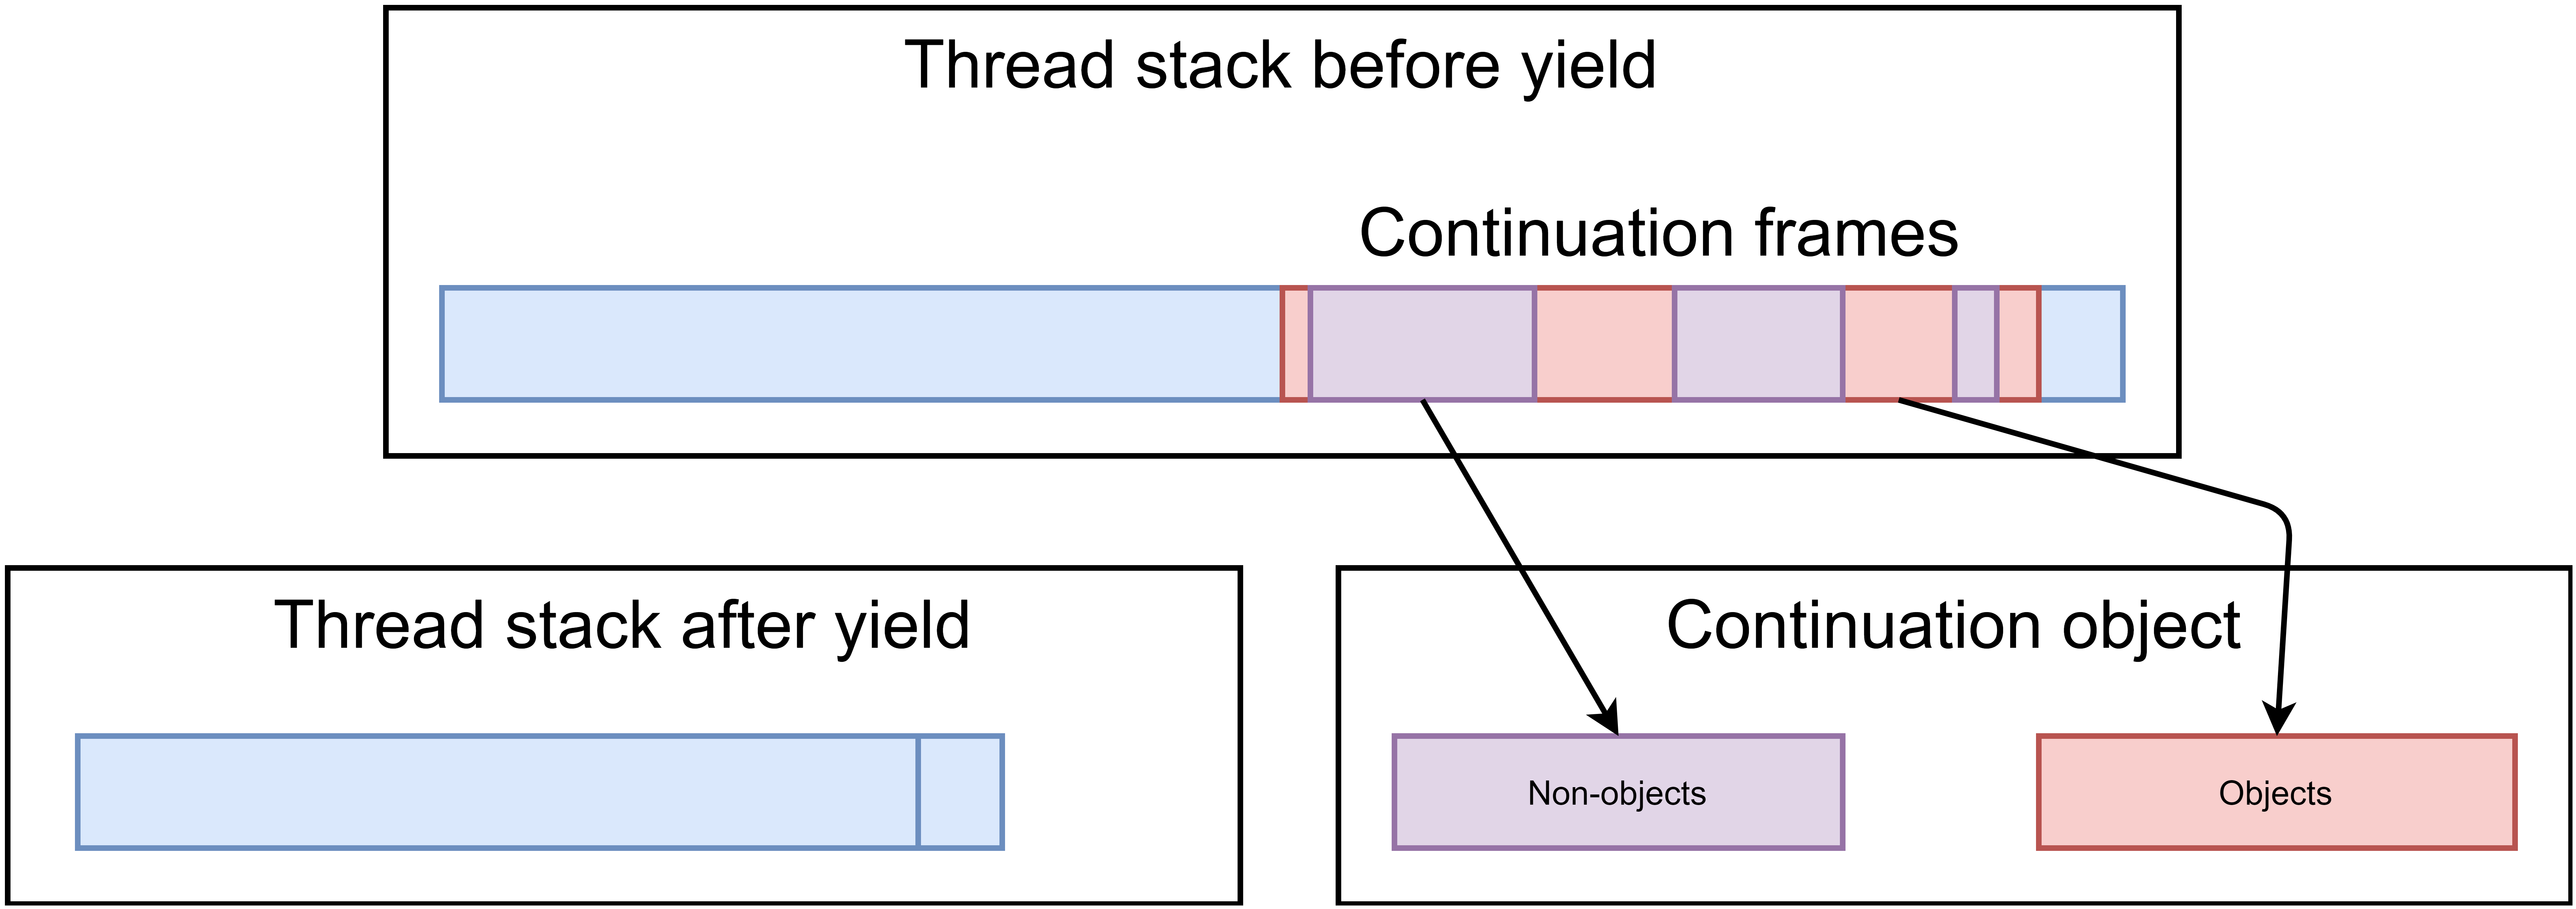
\includegraphics[width=1.0\linewidth]{img/freeze-jvmls-2019.png}
    \end{subfigure}
    \caption{Freeze \cite{OpenJDK:jvmls:2019}}
    \label{freeze}
\end{figure}

Looking at the previously mentioned two stacks on code level: One stack is an integer array for primitive values and metadata. The other one is an object array for references. All stack related methods exist twice: Once for the integer array and once for the object array. The methods are very similar. Therefore this thesis will only explain one set of them, which is the integer set.
\\
\\
Project Loom uses an integer sp as a stack pointer. Every time the stack is changed, the stack pointer will be updated. This is done by using the fixDecreasingIndexAfterResize method. As an example observe fixDecreasingIndexAfterResize using the arguments: index = 5, oldLength = 10, newLength = 20. It returns 15. The new stack pointer is therefore 15. That means that if a stack size gets changed, the remaining values are inserted starting at the end.

\begin{lstlisting}[language=custom-java]
    private int sp = -1; // index into the h-stack

    private int fixDecreasingIndexAfterResize(int index, int oldLength, int newLength) {
        return newLength - (oldLength - index);
    }
\end{lstlisting}

\myparagraph{getStack}
The getStack method is used to expand the stack. First, the program will test, whether the stack is null. If that is the case, the stack has not been created yet. Then the program will create the stack and adjust the stack pointer. If the stack is not empty, the program will create a new stack, that is big enough to fit the old and the new frames. Then it will copy the old frames into the new stack. Afterwards, the continuation's stack is set to the new stack. The stack pointer will be updated. The return value is boolean. It is True when getStack succeded. The method fails when the old stack length is larger than the new one.

\myparagraph{resizeStack}
Similar to how the getStack method expands the stack, the resizeStack method shrinks it. In contrast to the getStack method, the resizeStack method is a void and does not require to return a boolean on whether it succeeded or not.

\myparagraph{maybeShrink}
The maybeShrink method is called after yielding. It checks whether the stack size is bigger than a watermark it keeps track of. If it is, the watermark will be set to the stack size. Therefore if maybeShrink is called without adjusting the watermark, that means, that the stack size has not increased since the last time. If maybeShrink is called ten times without adjusting the watermark, the resizeStack method will be called with the watermark as it's argument.

\subsection{Critical Sections}
Project Loom solves critical sections with a classic semaphore design. The method pin increments the semaphore cs and the method unpin decrements it.

\begin{lstlisting}[language=custom-java]
    private short cs; // critical section semaphore

    public static void pin() {
        Continuation cont = currentCarrierThread().getContinuation();
        if (cont != null) {
            if (cont.cs == Short.MAX_VALUE)
                throw new IllegalStateException("Too many pins");
            cont.cs++;
        }
    }

    public static void unpin() {
        Continuation cont = currentCarrierThread().getContinuation();
        if (cont != null) {
            if (cont.cs == 0)
                throw new IllegalStateException("Not pinned");
            cont.cs--;
        }
    }
\end{lstlisting}

\subsection{Intrinsics}
Project Loom uses intrinsics to increase performance. Usually, if there is an intrinsic version of a function, there will still be a non-intrinsic one. In this case, there are no non-intrinsic versions of the functions. The following functions are exclusively intrinsic and relevant for this thesis:
\begin{lstlisting}[language=custom-java]
    @HotSpotIntrinsicCandidate
    private static long getSP()

    @HotSpotIntrinsicCandidate
    private void doContinue() 

    @HotSpotIntrinsicCandidate
    private static int doYield(int scopes)
\end{lstlisting}

For the x86 platform the following functions in stubGenerator\_x86\_64.cpp create the bytecode for the intrinsic versions of the functions named above:

\begin{lstlisting}[language=C++]
    address generate_cont_getSP()

    address generate_cont_thaw(bool return_barrier, bool exception)

    RuntimeStub *generate_cont_doYield()
\end{lstlisting}

In these functions, the maintainers of project Loom use their macroassembler. The macroassembler class can be found in src/hotspot/cpu/x86/macroAssembler\_x86.cpp. The yield method also utilizes two other big classes. One is a codebuffer located in src/hotspot/cpu/x86/asm/codeBuffer.cpp and the other is a oopmap, used for garbage collection, located in src/hotspot/share/compiler/oopMap.cpp.
\\
Analyzing these functions goes beyond the scope of this thesis.

\subsection{Run}
When a continuation gets started or continued the run method is called.
First the run method mounts the continuation. Mounting is realized using a VarHandle, which atomically sets a boolean to true.
\\
\\
Afterwards the current carrier-thread's continuation has to be updated. As an example the current carrier-thread's continuation before the update will be called bar. The new continuation will be called foo.

\begin{lstlisting}[language=custom-java]
    Thread t = currentCarrierThread();
    if (parent != null) {
        if (parent != t.getContinuation())
            throw new IllegalStateException();
    } else
        this.parent = t.getContinuation();
    t.setContinuation(this);
\end{lstlisting}

foo is not supossed to have a parent at this point of time. If foo has a parent, that parent has to be bar. If it is not, something seriously went wrong and an error is thrown. The expected outcome is, that foo has no parent. In that case foo will become the child bar. Afterwards foo will become the current carrier-threads's continuation.

\begin{figure}[H]
    \centering
    \begin{subfigure}[b]{0.45\textwidth}
        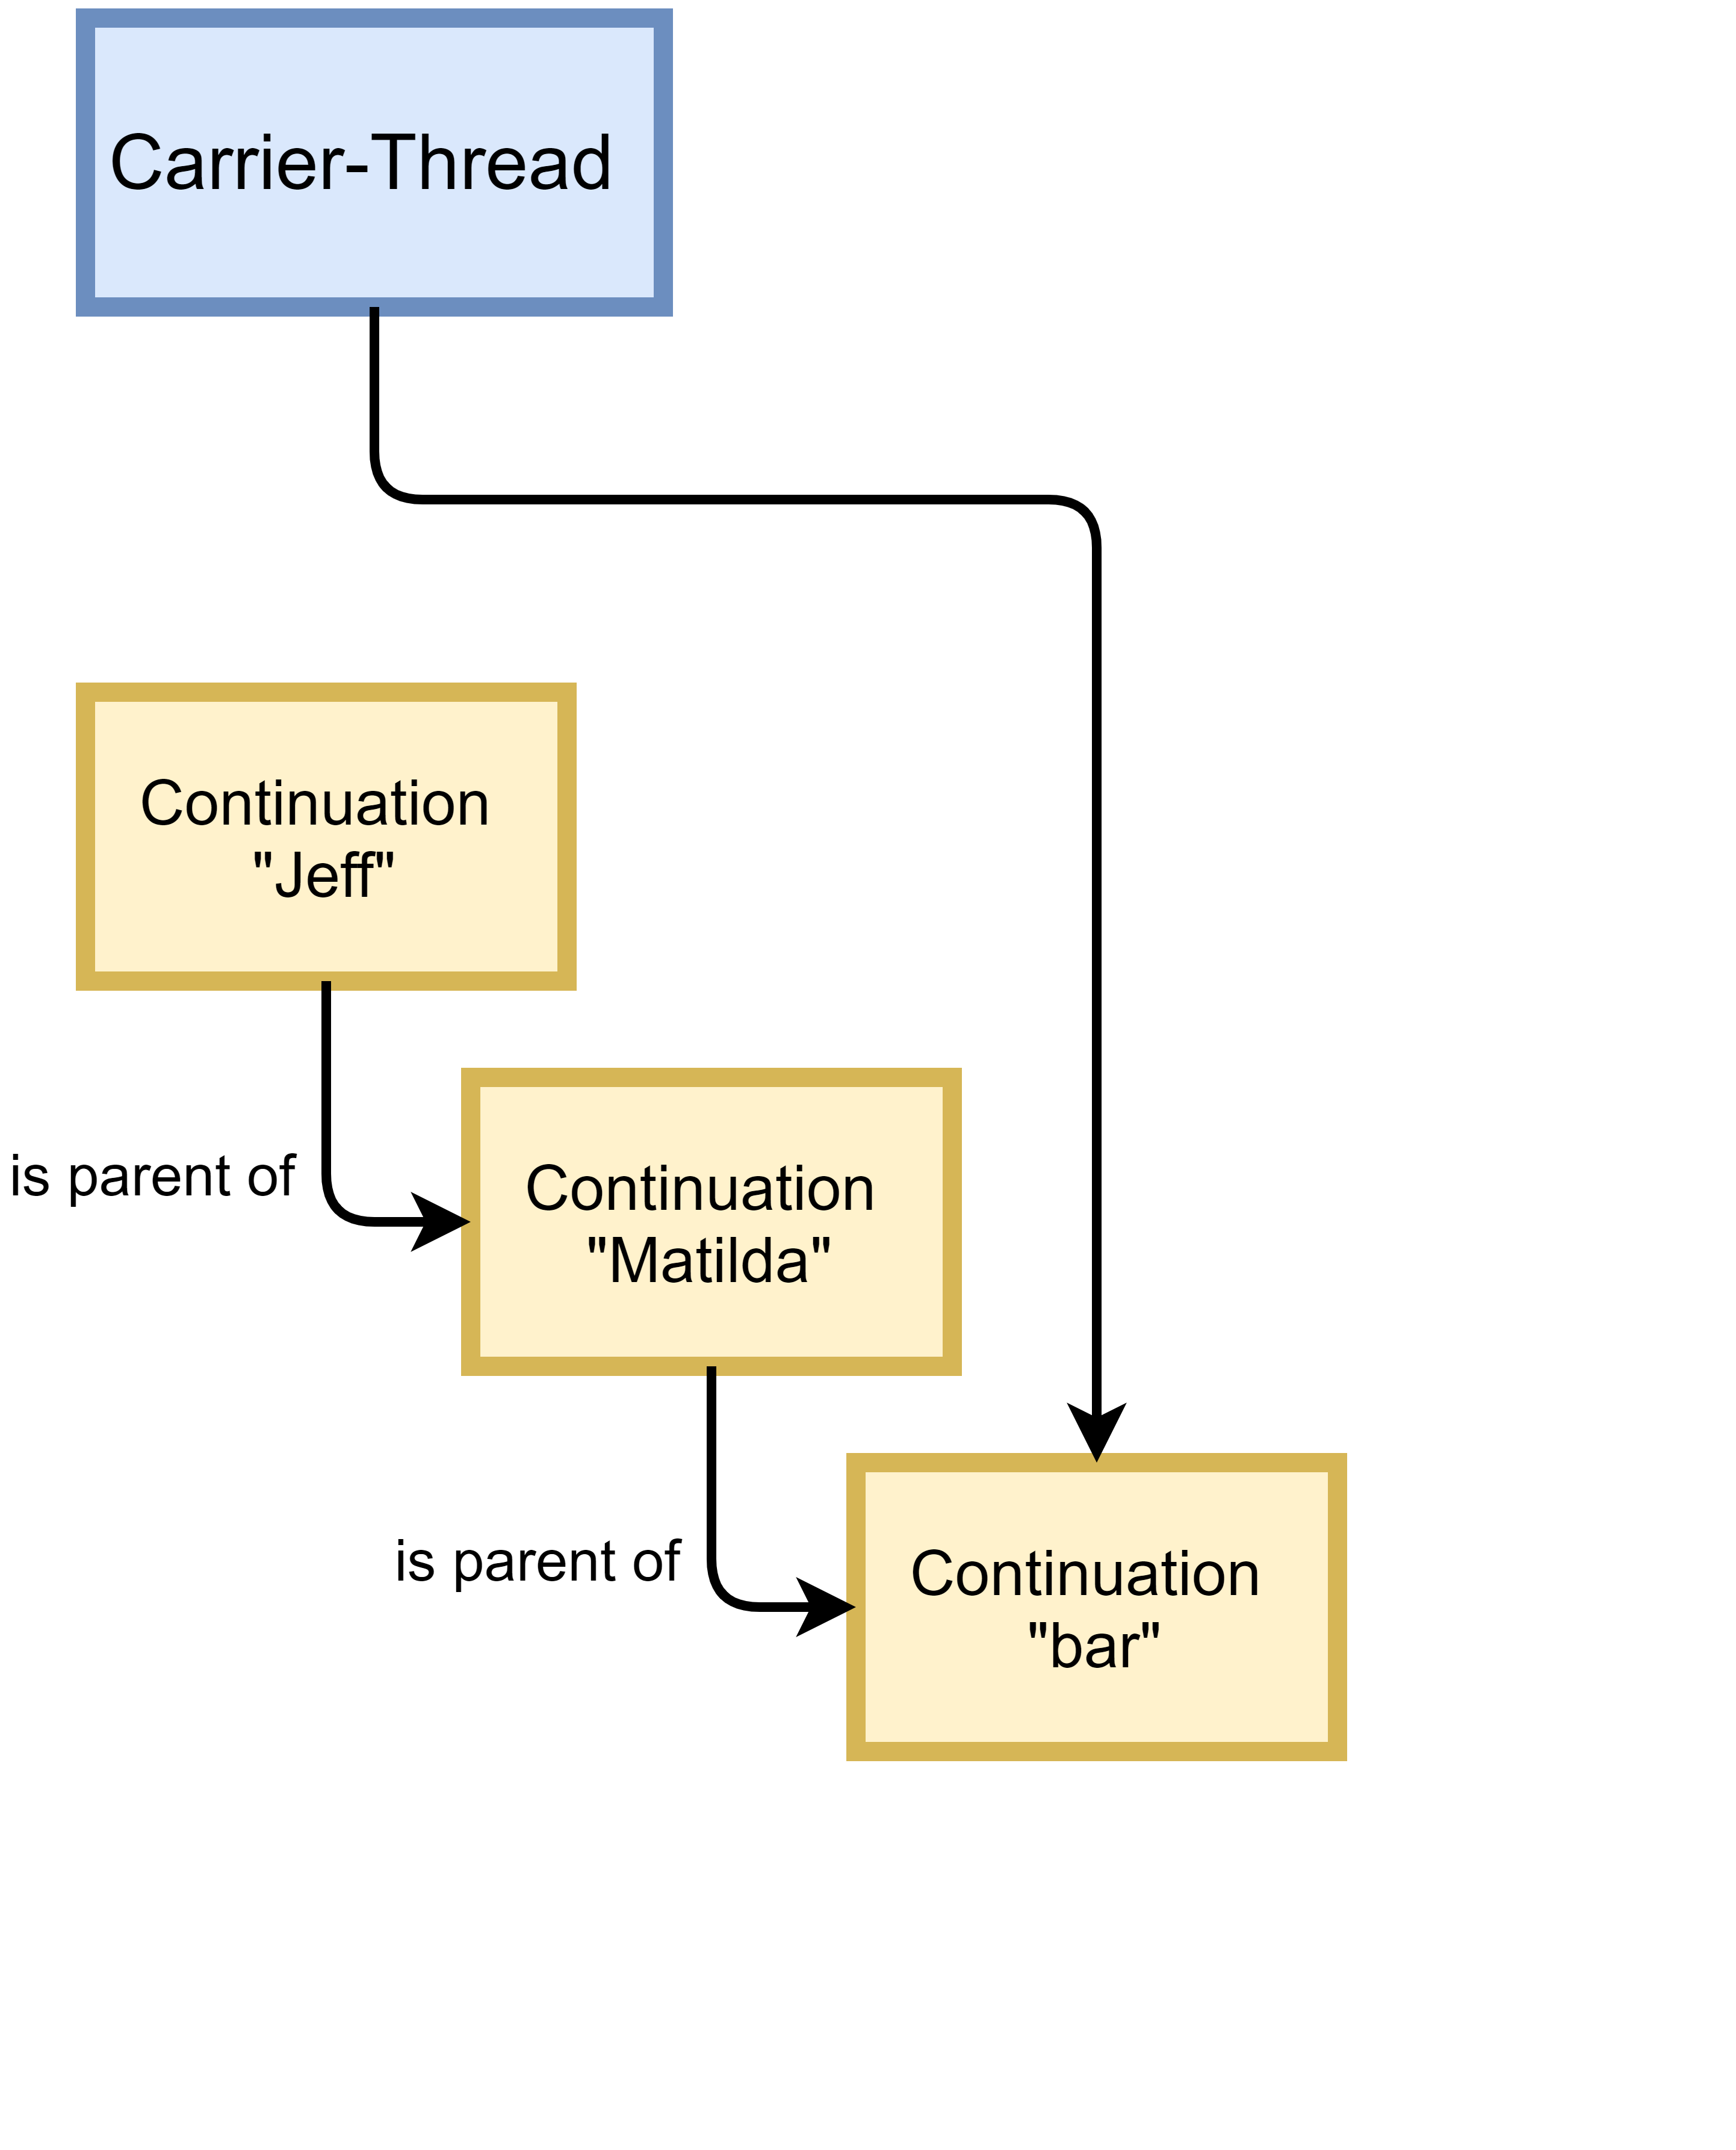
\includegraphics[width=1.0\linewidth]{img/before-run-changes-current-continuation.png}
        \label{Before Carrier-Thread's Continuation gets updated}
    \end{subfigure}
    \begin{subfigure}[b]{0.45\textwidth}
        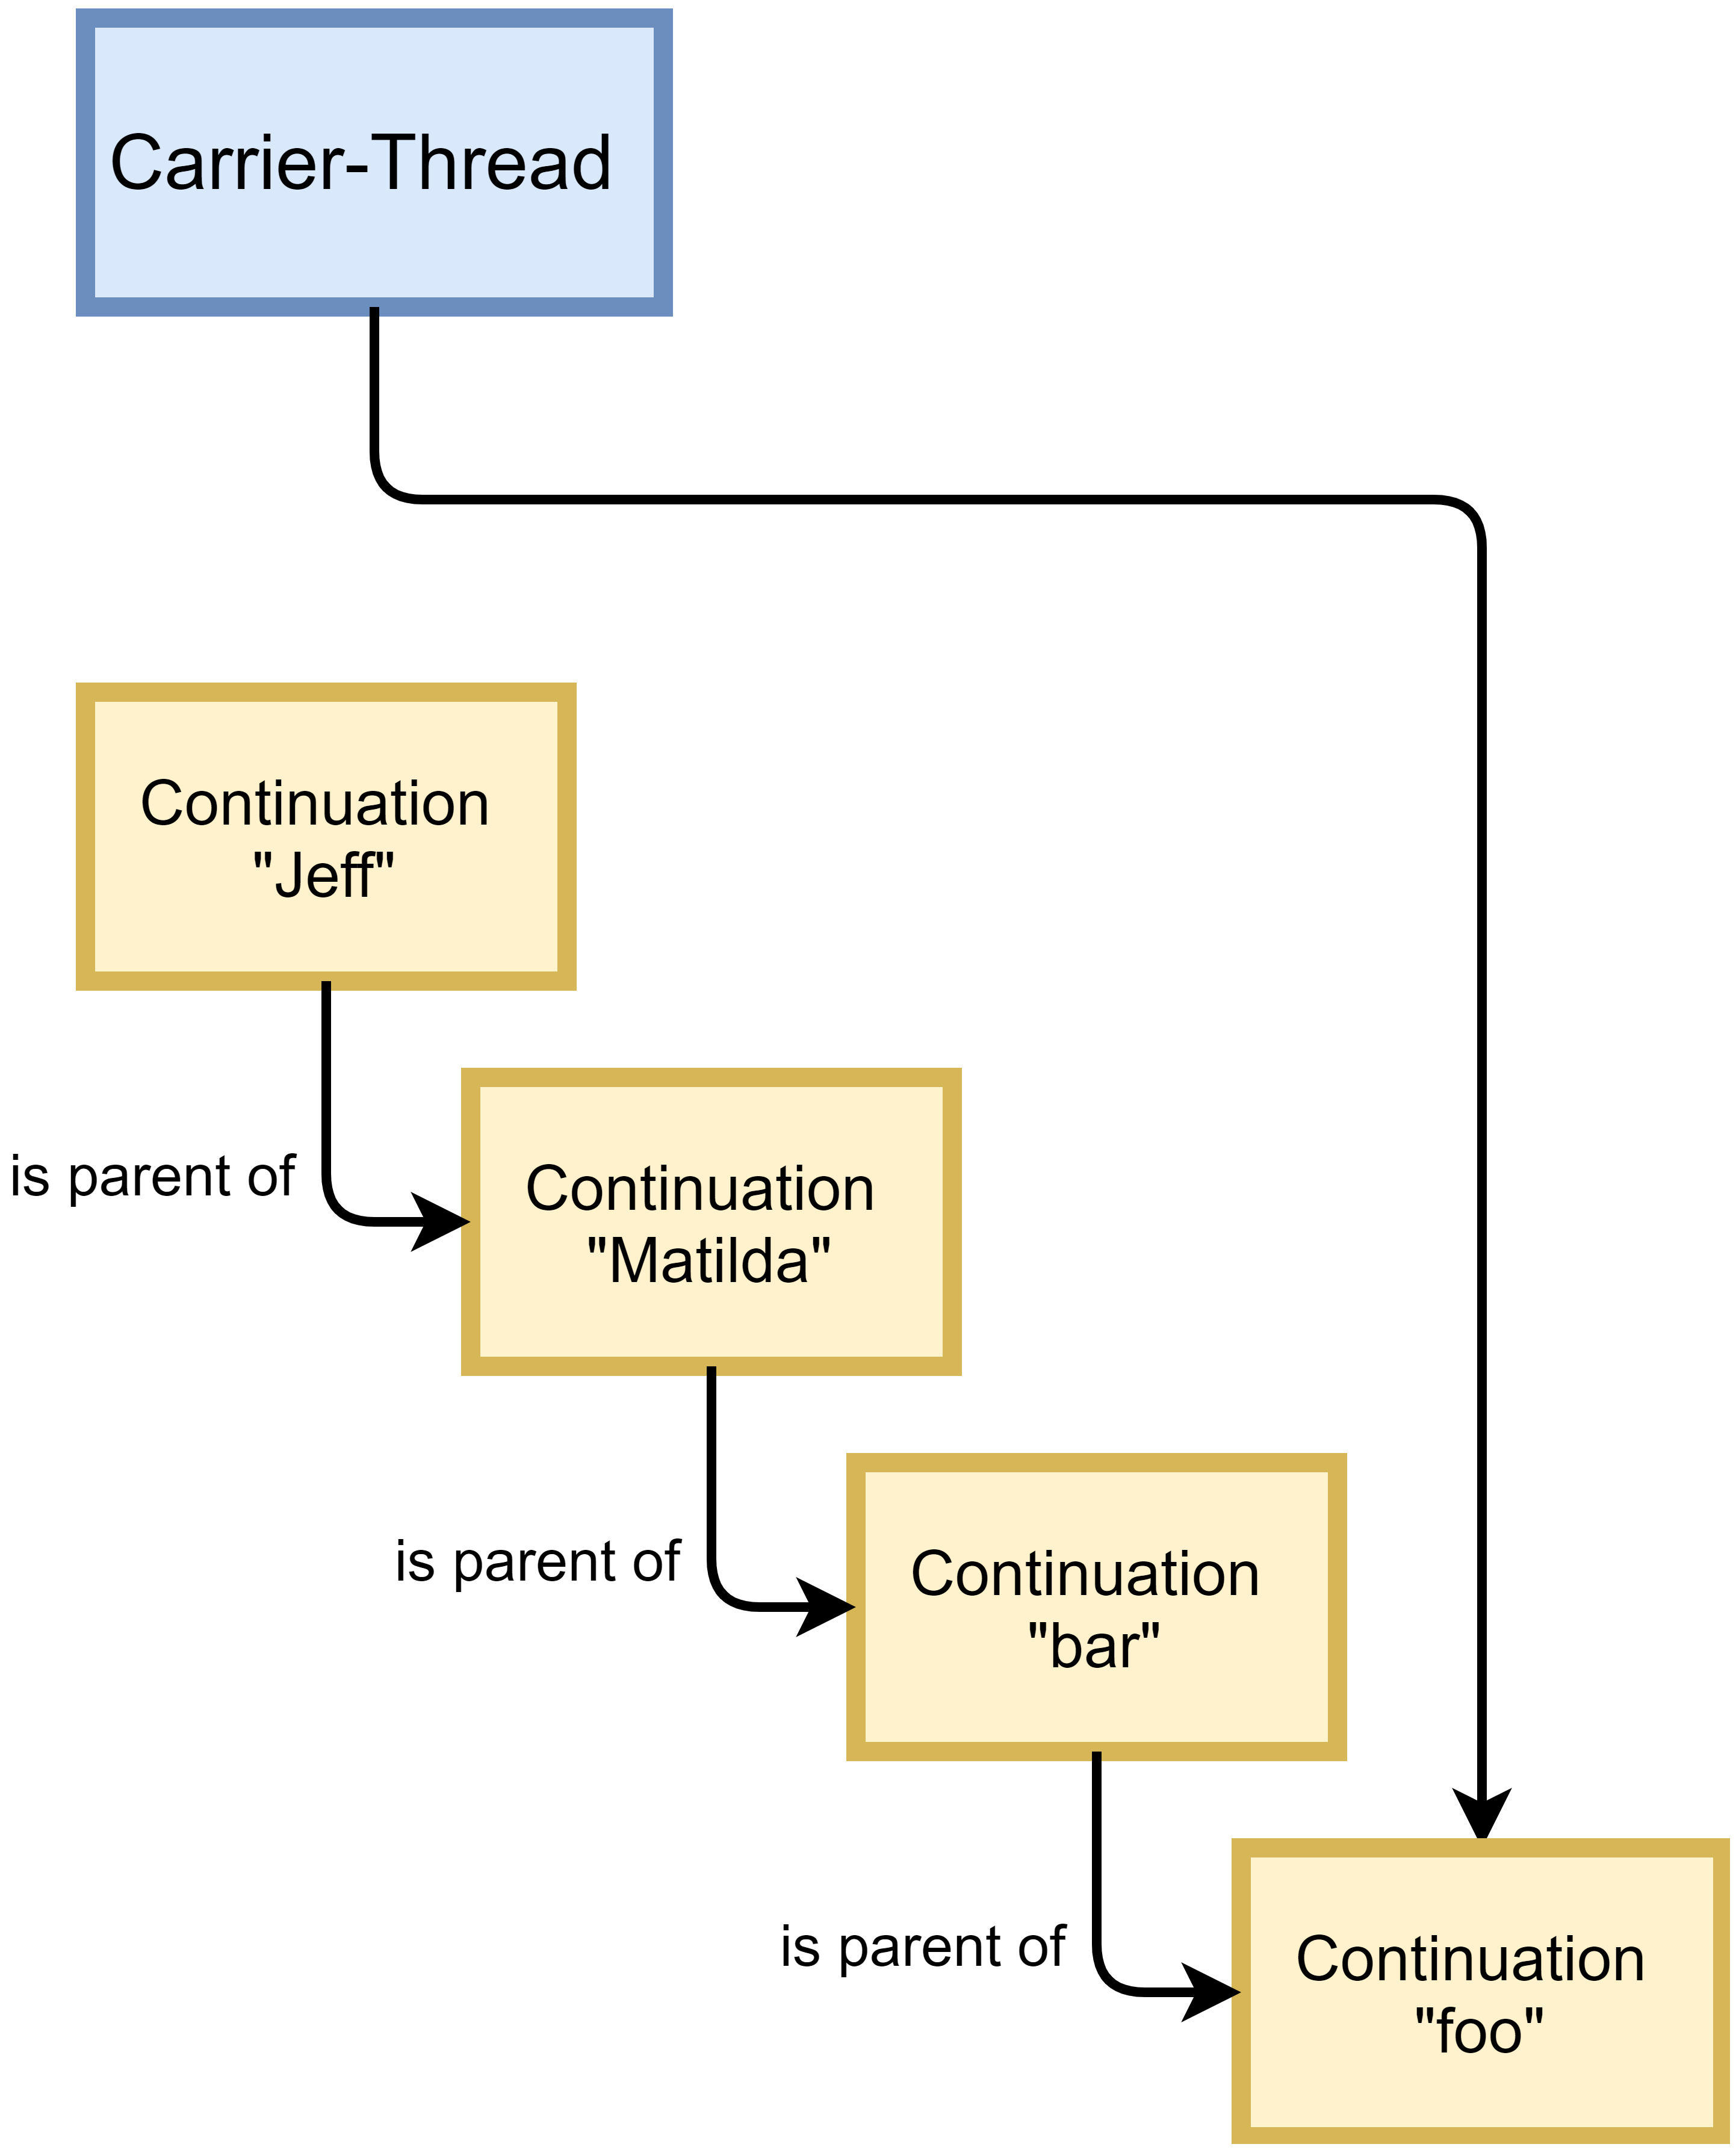
\includegraphics[width=1.0\linewidth]{img/after-run-changes-current-continuation.png}
        \label{After Carrier-Thread's Continuation gets updated}
    \end{subfigure}
    \caption{Carrier-Thread's Continuation gets updated}
\end{figure}

After that, the run method will call either the enter method or the continue method depending on whether foo is being started for the first time.
\\
\\
Once foo is done, it returns to the run method. The current carrier-thread's continuation will be set to bar. foo will be removed as a child of bar. Finally, foo will be unmounted, similar to how it was mounted at the beginning.

\subsection{Yield}
Project Loom uses three different yield functions, which are always called in the same order.
\\
First \lstinline[basicstyle=\ttfamily\color{blue}]{public static boolean yield(ContinuationScope scope)} is called. This method checks, if the current carrier-thread's continuation is part of the given ContinuationScope scope. This is done by looping a variable c through the parents of the current carrier-thread's continuation. The loop stops once c is either null or the scope of c is the same as the given scope. If c ends up being null, that means, that the program is being told to yield a ContinuationScope, while it is running a continuation, that is not part of that scope. This is undesired behavior and throws an exception. If c is not null, the program can continue and the second function will be called.
\\
\\
The other two functions are beyond the scope of this thesis, because they either are completely intrinsic or because they utilize variables that are returned from intrinsics.


\subsection{Continue}
The continue method is entirely intrinsic. Therefore it is beyond the scope of this thesis.




\section{Virtual Thread}

Similar to how threads were created as lightweight processes, virtual threads were created as lightweight threads. Therefore they line up in the hierarchy right behind the kernel threads.
\begin{figure}[H]
    \centering
    \begin{subfigure}[b]{1.0\textwidth}
        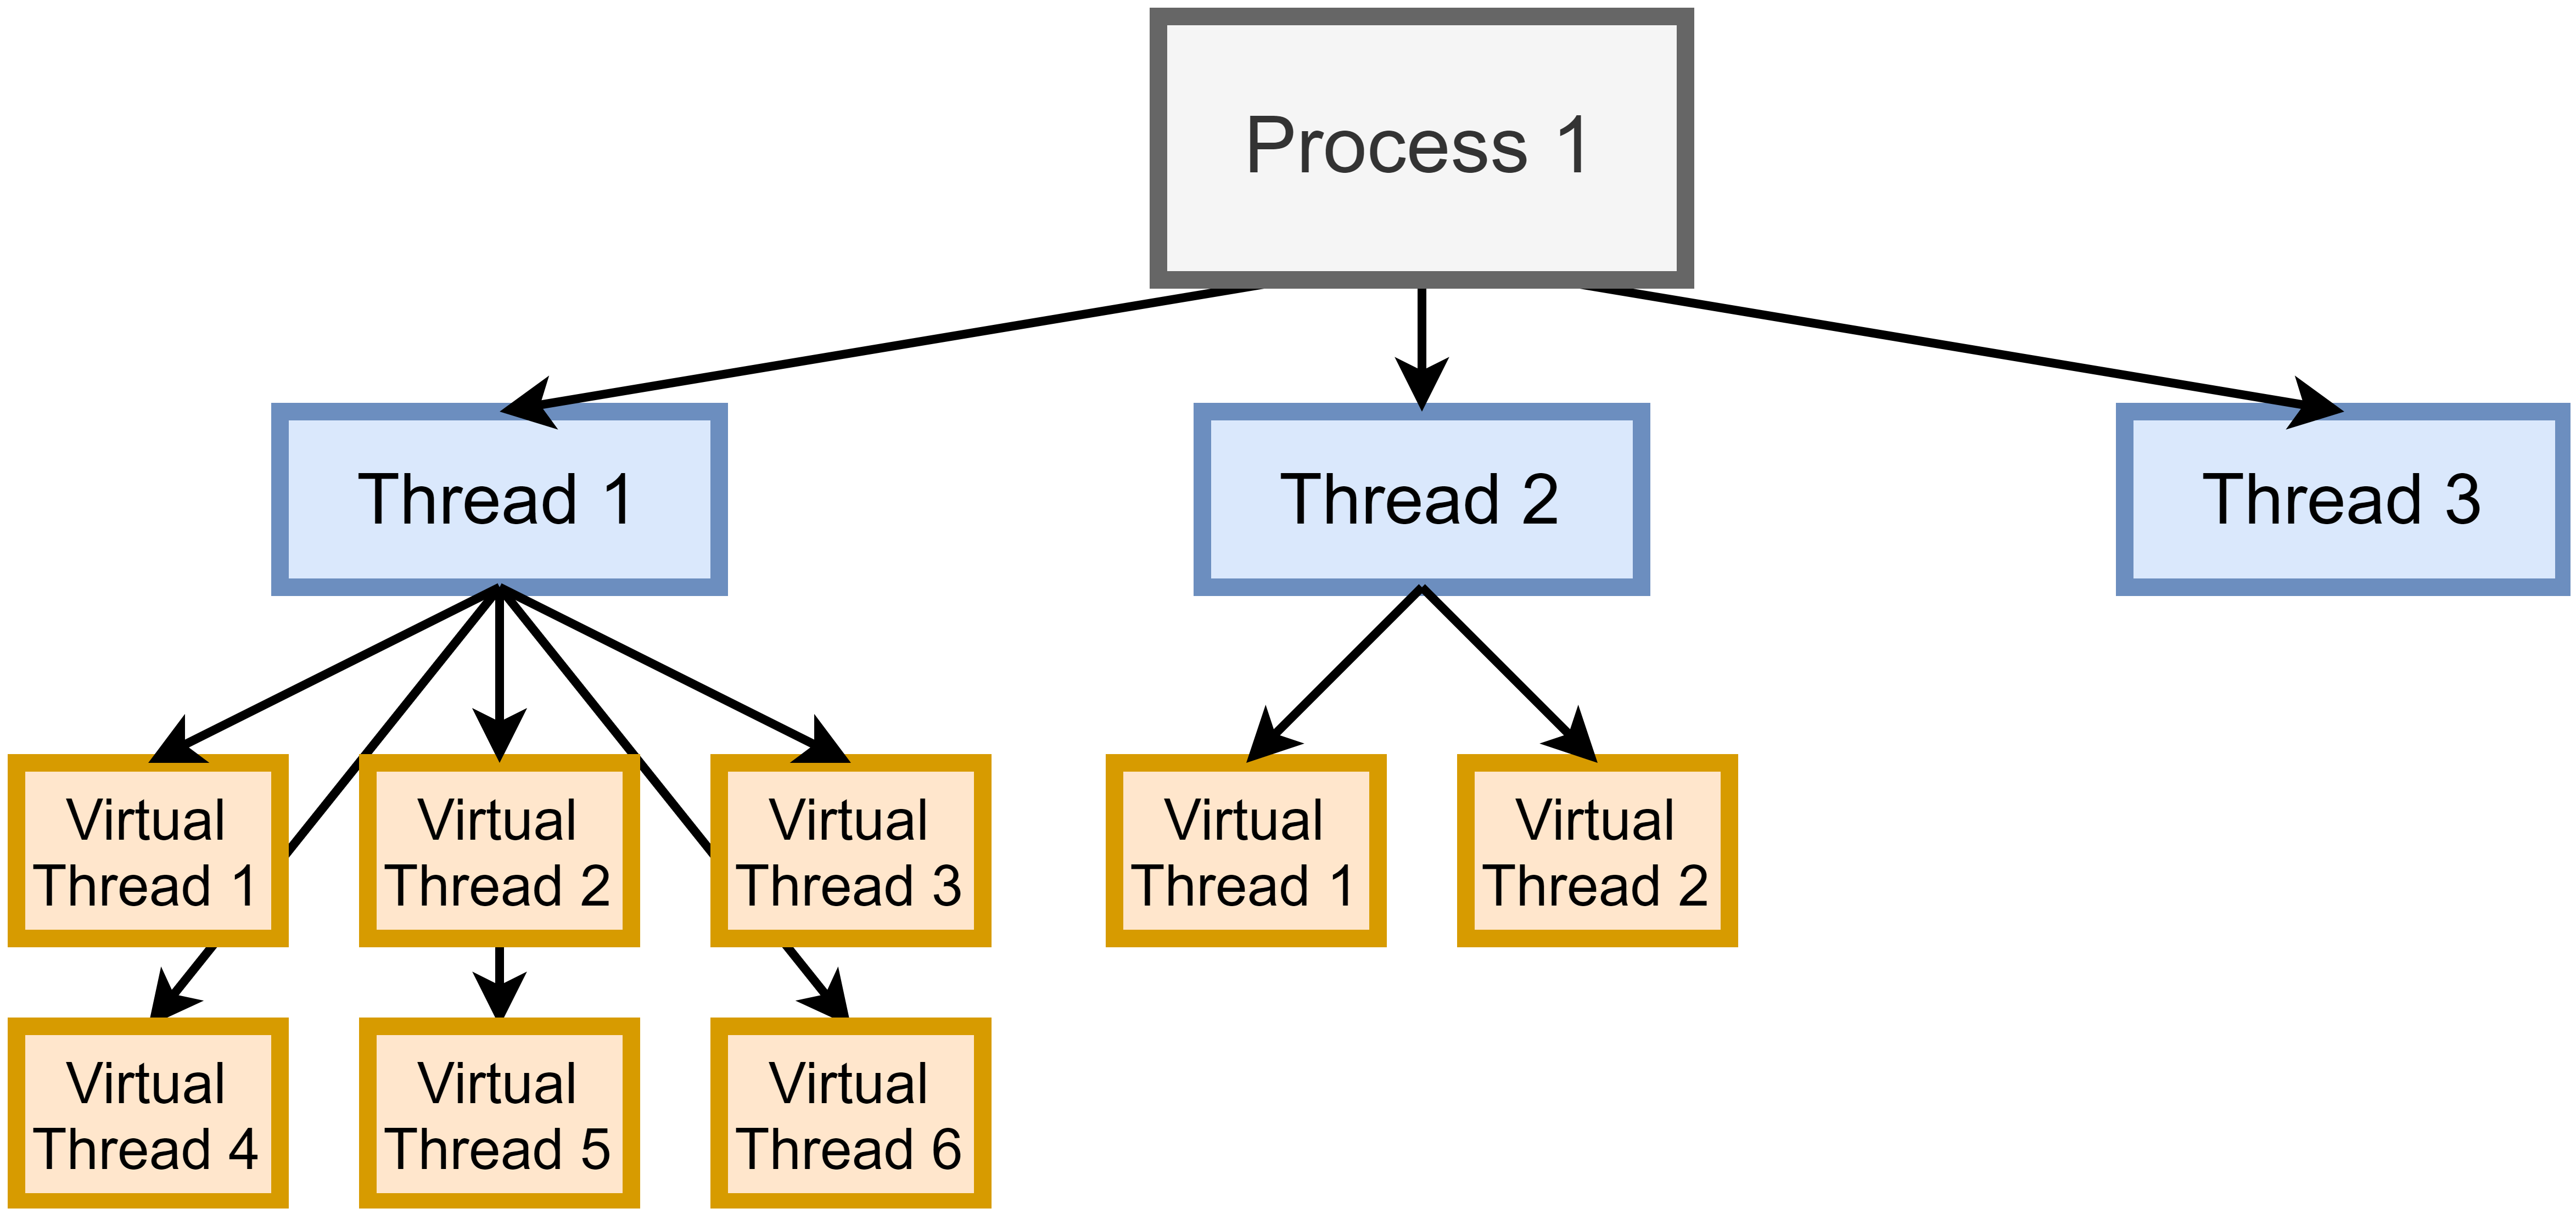
\includegraphics[width=1.0\linewidth]{img/process-thread-vthread.png}
    \end{subfigure}
    \caption{Process - Thread - Virtual Thread - Hierarchy}
    \label{Process - Thread - Virtual Thread - Hierarchy}
\end{figure}
Similar to how the scheduler of an operating system allocates CPU time to each kernel thread, the JVM allocates CPU time to each virtual thread. The scheduler is not the focus of this work. It will be briefly addressed in the next chapter.
\begin{figure}[H]
    \centering
    \begin{subfigure}[b]{1.0\textwidth}
        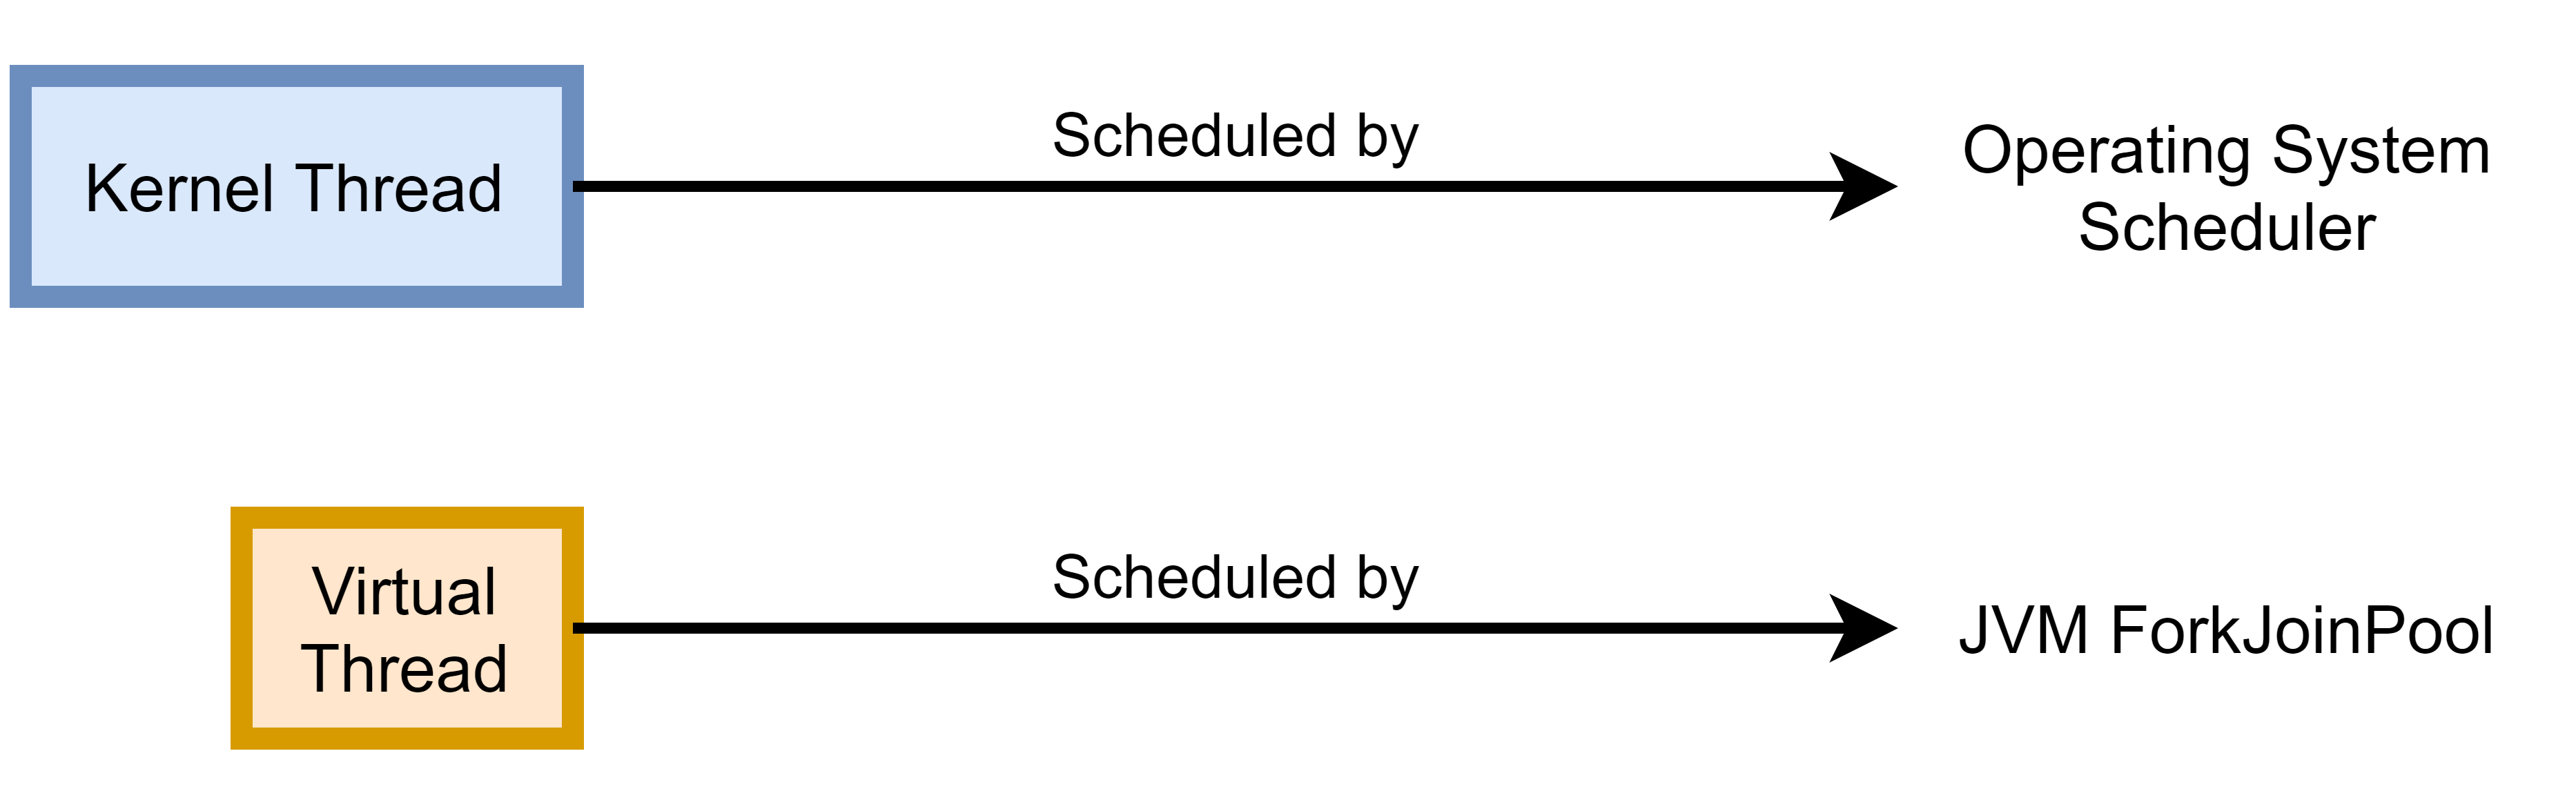
\includegraphics[width=1.0\linewidth]{img/thread-vthread-scheduler.png}
    \end{subfigure}
    \caption{Thread - Virtual Thread - Scheduler}
    \label{Thread - Virtual Thread - Scheduler}
\end{figure}
The virtual thread class is a high level class. Underneath it the low level continuation class is at work. Direct interaction with the continuation class is currently possible, but developers are advised to use virtual threads instead. QUOTE: Continuations will probably move to a non-exported package at some point (stand in einer email, wahrscheinlich direkt an ihn selbst addressiert gewesen, wie zitieren?)




\subsection{Examples}

\myparagraph{Virtual Thread vs Kernel Thread}
The following code excerpt shows very well, how simple the transition from kernel to virtual threads is envisioned to be by project Loom.

\begin{lstlisting}[language=custom-java]
    Runnable printThread = () -> System.out.println(Thread.currentThread());

    var virtualThreadFactory = Thread.builder().virtual().factory();
    var kernelThreadFactory = Thread.builder().factory();

    var virtualThread = virtualThreadFactory.newThread(printThread);
    var kernelThread = kernelThreadFactory.newThread(printThread);

    virtualThread.start();
    kernelThread.start();
\end{lstlisting}
The code above first creates a Runnable called printThread.
Then a ThreadFactory is created for both kernel and virtual threads.
These ThreadFactories are used to create a virtual and a kernel thread.
Afterwards, both threads are started. \cite{Baeldung:Threads}

\subsection{Structured Concurrency}
The ExecutorService class can be used to bring structured concurrency to virtual threads.
\\
\\
Here, the program will only continue once both tasks inside the try-block are finished.

\begin{lstlisting}[language=custom-java,caption={Structured Concurrency - Simple \cite{loom:structured-concurrency}},captionpos=b]
    ThreadFactory factory = Thread.builder().virtual().factory()

    try (ExecutorService executor = Executors.newUnboundedExecutor(factory)) {
        executor.submit(task1);
        executor.submit(task2);
    }
\end{lstlisting}

Here, the main program will only continue once foo and bar are done. Similar to that foo and bar are only going to be done, once the methods inside their try-blocks are done.
\begin{lstlisting}[language=custom-java,caption={Structured Concurrency - Nested \cite{loom:structured-concurrency}},captionpos=b]
    ThreadFactory factory = Thread.builder().virtual().factory()

    try (ExecutorService executor = Executors.newUnboundedExecutor(factory)) {
        executor.submit(() -> foo());
        executor.submit(() -> bar());
    }

    void foo() {
        try (ExecutorService executor = Executors.newUnboundedExecutor(factory)) {
            executor.submit(...);
        }
    }

    void bar() {
        try (ExecutorService executor = Executors.newUnboundedExecutor(factory)) {
            executor.submit(...);
        }
    }
\end{lstlisting}

This example works very similar to the first one. The only change is, that a deadline of 30 seconds has been added. Once the deadline is hit, all tasks inside the try block are going to be canceled. If those tasks started additional tasks inside themselves, those tasks will also be canceled.

\begin{lstlisting}[language=custom-java,caption={Structured Concurrency - Deadlines \cite{loom:structured-concurrency}},captionpos=b]
    ThreadFactory factory = Thread.builder().virtual().factory()
    var deadline = Instant.now().plusSeconds(30);

    try (ExecutorService executor = Executors.newUnboundedExector(factory).withDeadline(deadline)) {
        executor.submit(task1);
        executor.submit(task2);
    }
\end{lstlisting}


\section{ForkJoinPool}
Per default virtual threads use the Java ForkJoinPool as their scheduler. Project Loom considers this scheduler to be "excellent" \cite{loom:proposal}. Knowledge regarding the ForkJoinPool is not necessary to work with virtual threads. The creation and maintenance of the scheduler is part of the virtual thread class. However, if a developer wants to use their own scheduler, it is easily possible:

\begin{lstlisting}[language=custom-java]
    CustomScheduler scheduler = new CustomScheduler();
    ThreadFactory factory = Thread.builder().virtual(scheduler).factory();
\end{lstlisting}

The developer creates an instance of their custom scheduler and passes it as an argument when creating the ThreadFactory.
















    \chapter{Evaluation}

\section{Continuation Benchmarks}
These are benchmarks made by project Loom themselves using the JMH.
The benchmark contains five different classes:
\begin{itemize}
  \item Freeze
  \item Thaw
  \item FreezeAndThaw
  \item OneShot
  \item Oscillation
\end{itemize}

All classes use the same settings:
\begin{lstlisting}[language=custom-java]
    @BenchmarkMode(Mode.AverageTime)
    @OutputTimeUnit(TimeUnit.NANOSECONDS)
    @State(Scope.Thread)
    @Warmup(iterations = 5, time = 1, timeUnit = TimeUnit.SECONDS)
    @Measurement(iterations = 5, time = 1, timeUnit = TimeUnit.SECONDS)
    @Fork(1)
\end{lstlisting}
They measure the average time and return the results in nanoseconds. They run five warmup iterations before measuring. Each measurement is ran five times. The state is the default state. Forking is enabled.
\\
\\
Each class contains at least one function which is benchmarked multiple times using different parameters.
All classes except for the Oscillation class use the same two parameters. Those parameters are called paramCount and stackDepth:
\begin{lstlisting}[language=custom-java]
    @Param({"1", "2", "3"})
    public int paramCount;
    
    @Param({"5", "10", "20", "100"})
    public int stackDepth;
\end{lstlisting}
Measurement series are run for every combination of those two parameters. Resulting in 12 different measurements.
The parameters of the Oscillation class class are sligthly different:
\begin{lstlisting}[language=custom-java]
    @Param({"2", "3", "4"})
    public int minDepth;
    
    @Param({"5", "6", "7", "8"})
    public int maxDepth;
    
    @Param({"10", "100", "1000"})
    public int repeat;
\end{lstlisting}
This results in 36 runs for the Oscillation class.
\\
\\
All classes use the same core task to benchmark. It is a simple recursive function. For example, if the stackDepth is 10, the function will call itself 10 times. Depending on the paramCount and which class is being benchmarked, the recursive function will then perform certain actions at a certain stackDepth.
\\
\\
Errors of the following results can be found in the annex.
\subsection{Freeze}
The Freeze benchmark optionally yields at a certain depth. It only measures yielding. An increase in the parameter count was expected to increase the time it takes to freeze since there are more frames to copy. This behavior can only be observed at a stack depth of 100. Measurement inaccuracies might be to blame for that. An increase in stack depth consistently increases the time it takes to finish the task, as expected.

\begin{figure}[H]
  \centering
  \begin{subfigure}[b]{1.0\textwidth}
    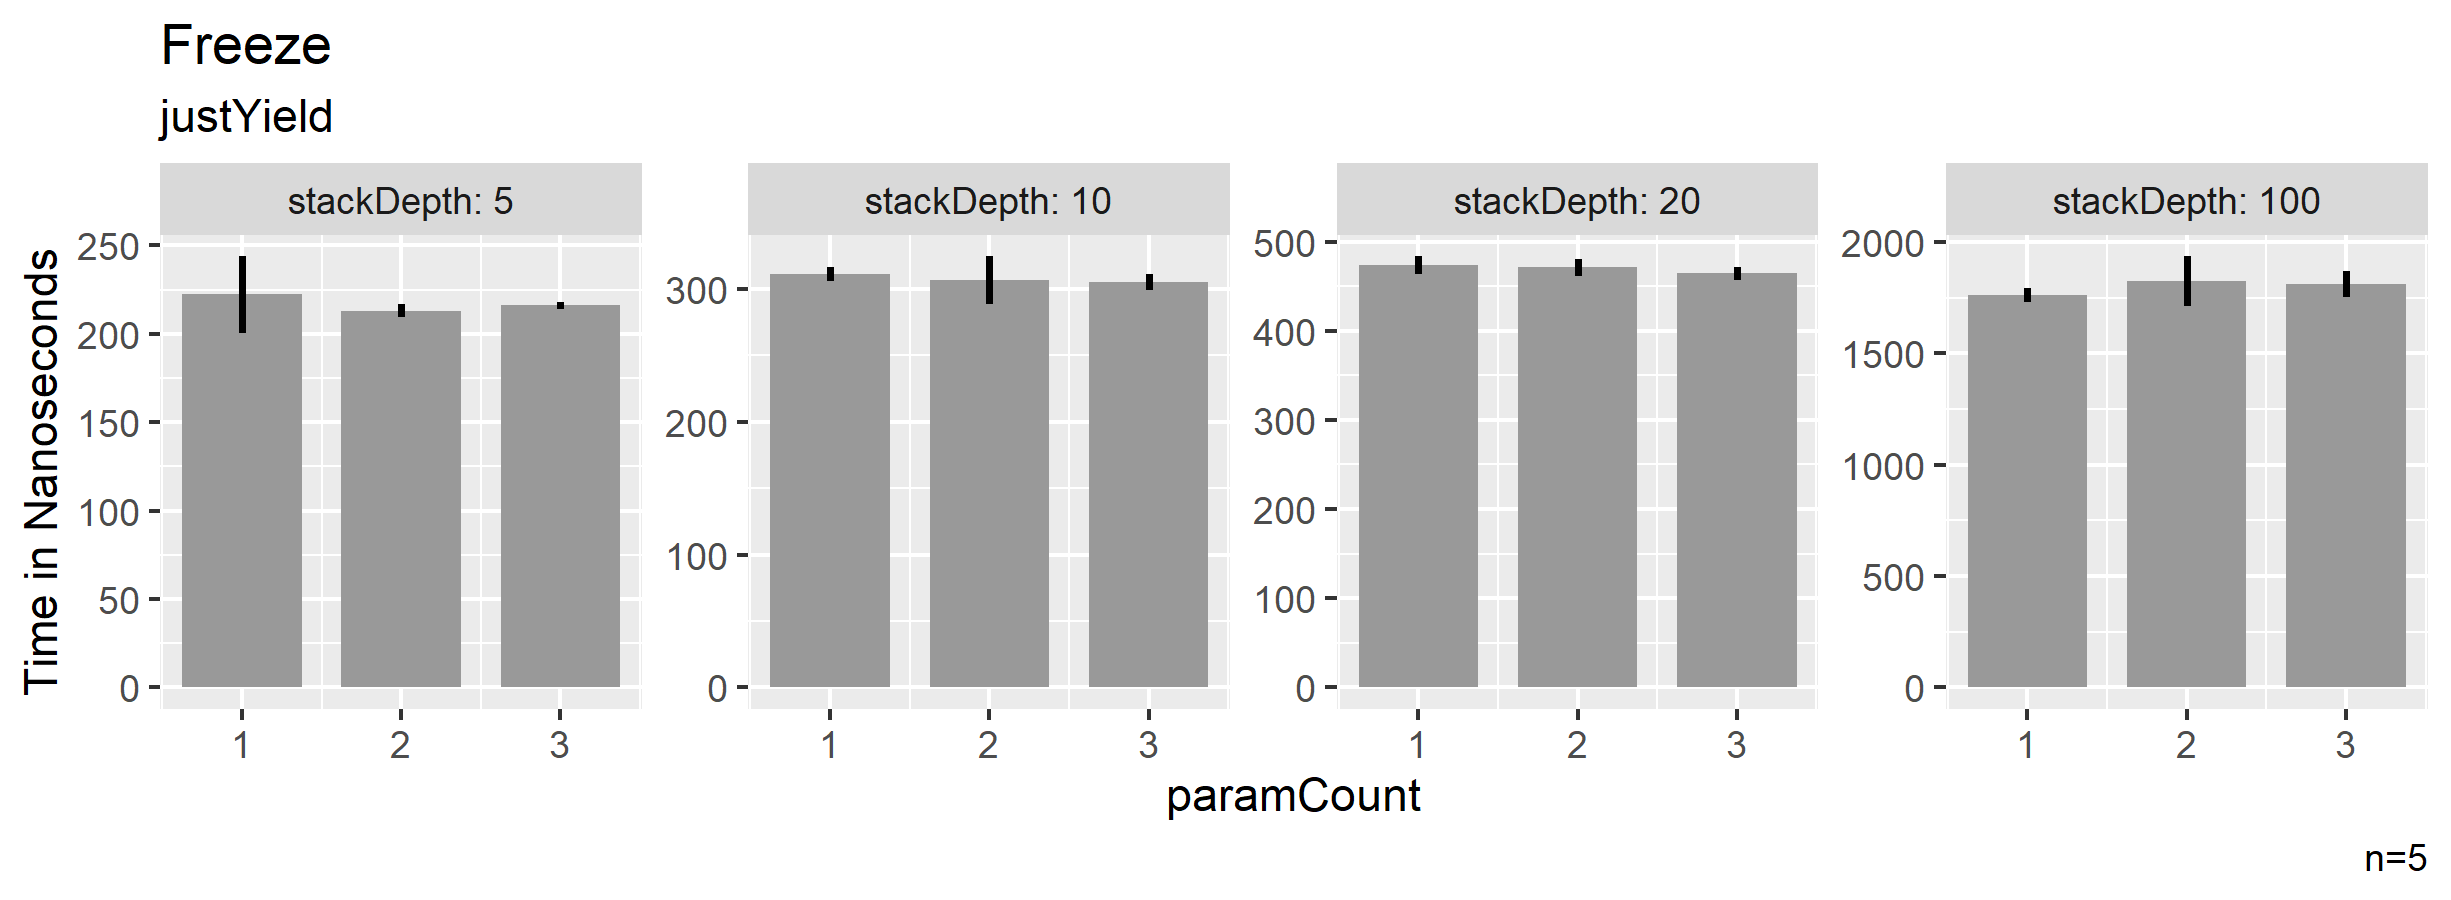
\includegraphics[width=1.0\linewidth]{img/jmh/Freeze.png}
  \end{subfigure}
  \caption{Freeze}
\end{figure}


\subsection{Thaw}
Similar to how the Freeze benchmark only measures yielding, the Thaw benchmark only measures the reverse, which is continuing. The expectations here were the same as before: Both an increase in parameter count and an increase in stack depth should increase the time. This time around only at a stack depth of 5 the results were different from the expectations.

\begin{figure}[H]
  \centering
  \begin{subfigure}[b]{1.0\textwidth}
    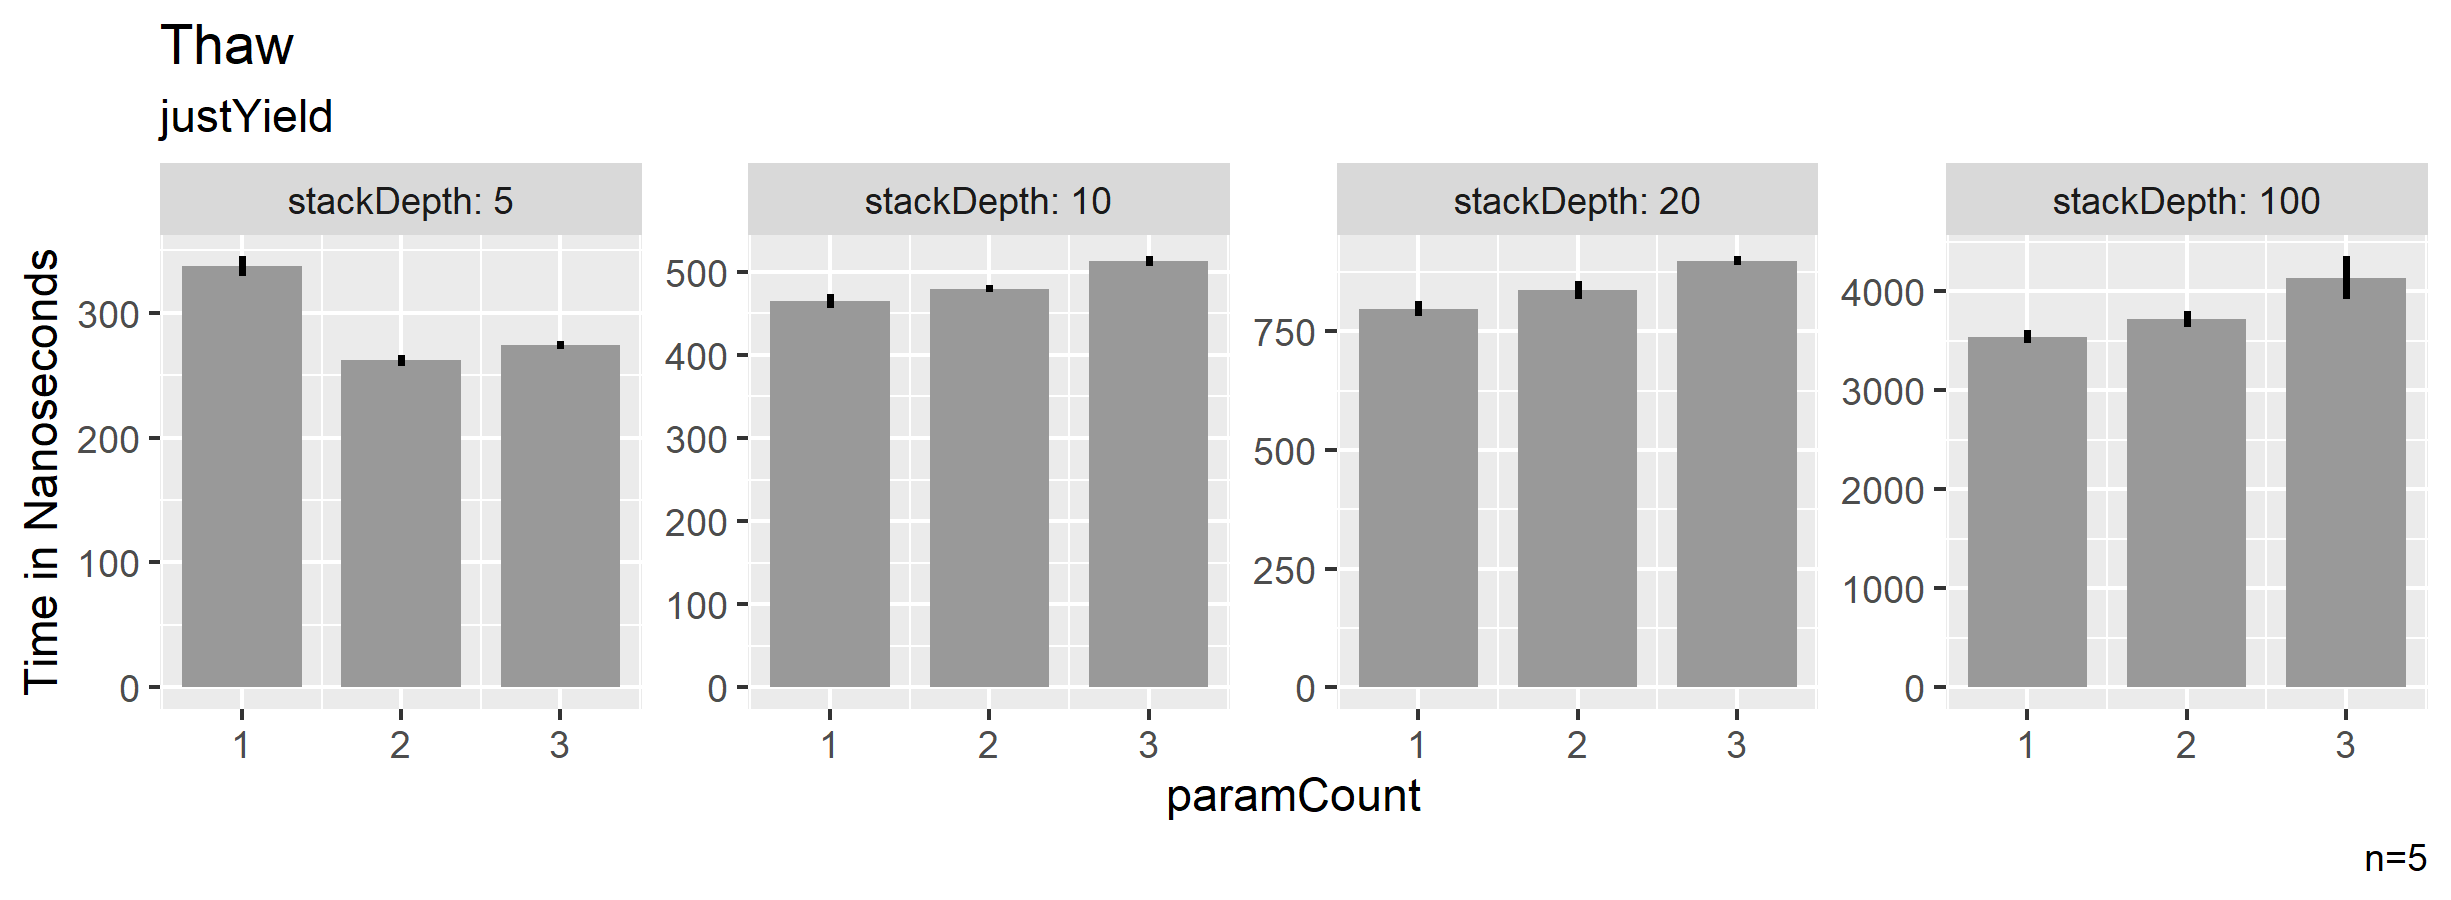
\includegraphics[width=1.0\linewidth]{img/jmh/Thaw.png}
  \end{subfigure}
  \caption{Thaw}
\end{figure}

\subsection{FreezeAndThaw}
As the name implies FreezeAndThaw measures both freezing and thawing. It runs two different methods: baseline and yieldAndContinue. The difference between those two is, that the continuation of the baseline method doesn't yield at the limit. Which means it doesn't yield at all. It just completes the task. So one can compare the baseline and the yieldAndContinue run to see how strongly freezing and thawing affected the time to finish the task. As one can see in the figure below, the impact of yielding and continuing is big. Without it, the task is completed up to 10 times faster.

\begin{figure}[H]
  \centering
  \begin{subfigure}[b]{1.0\textwidth}
    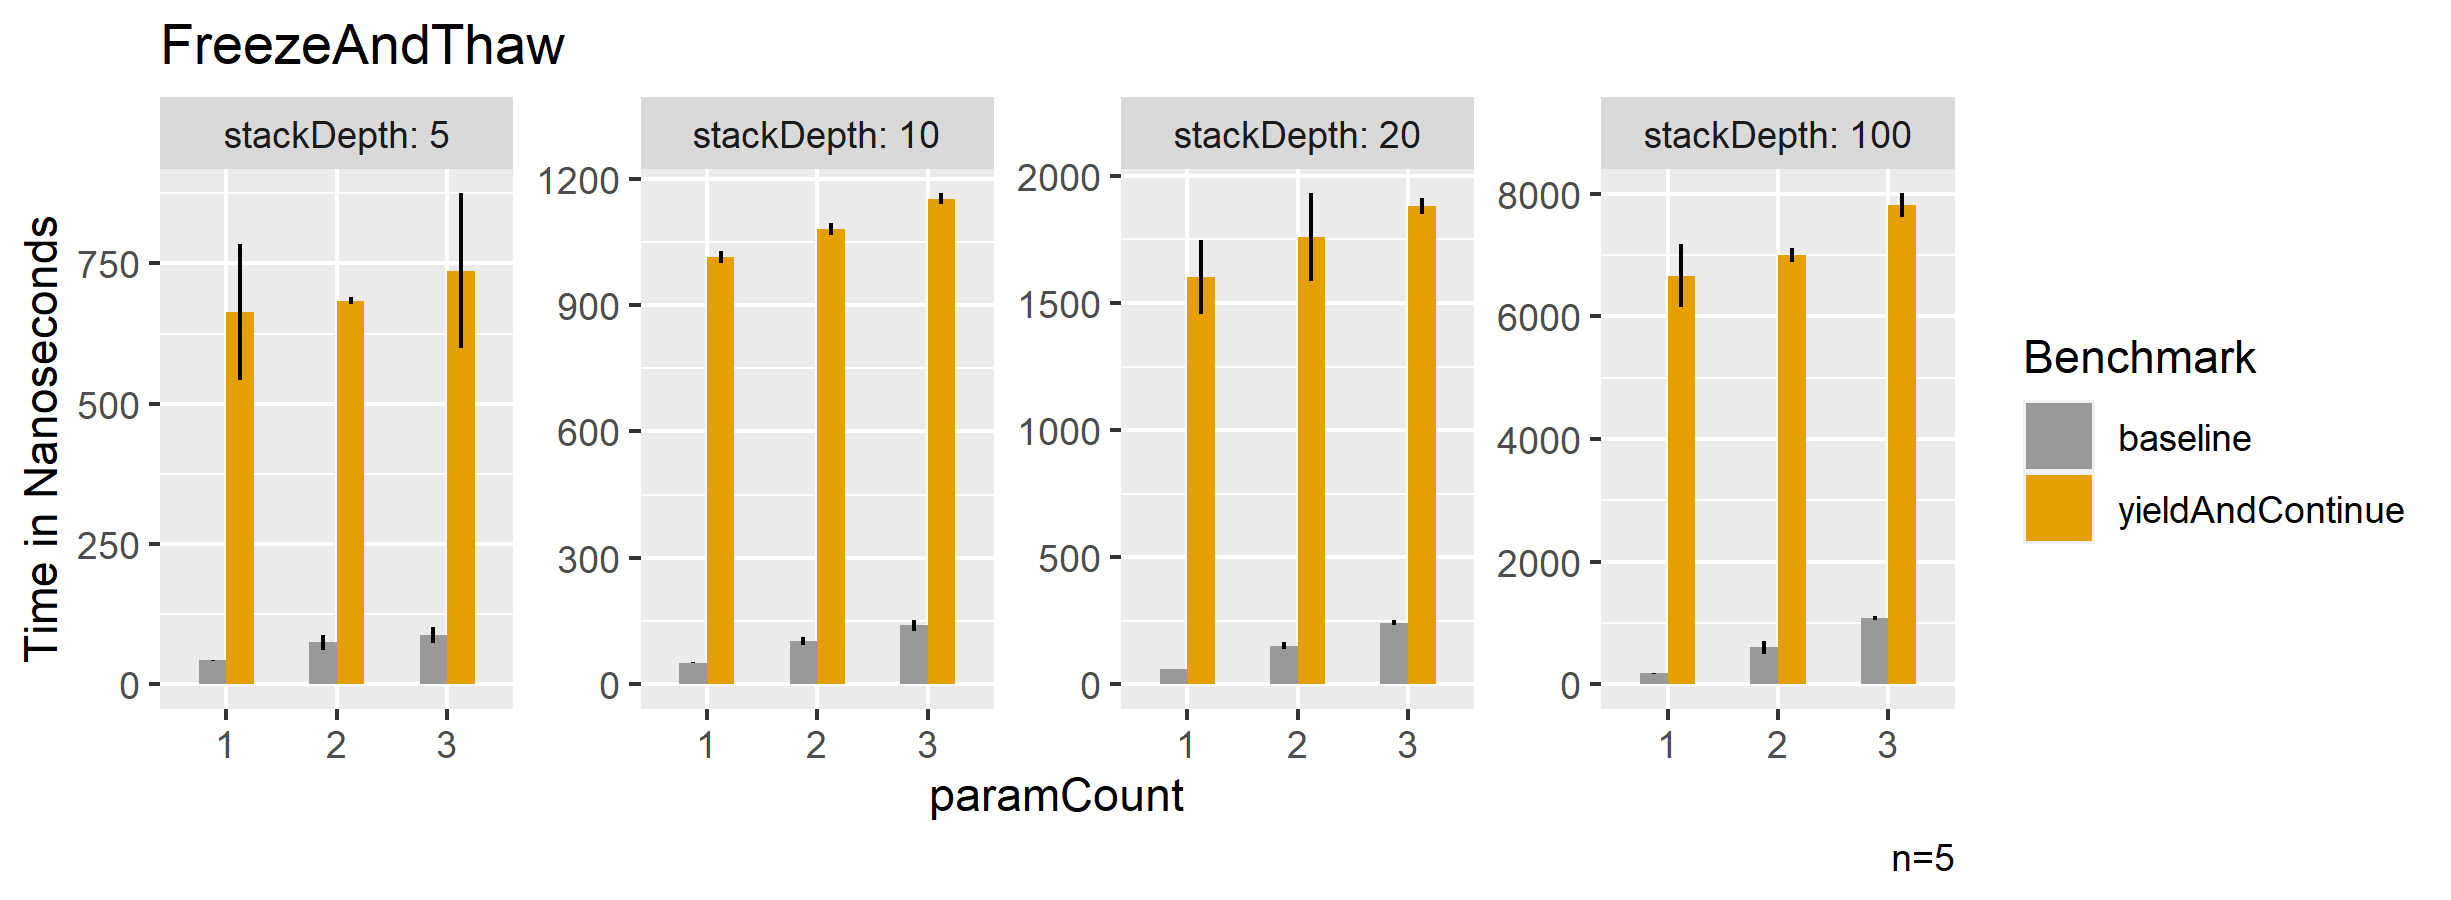
\includegraphics[width=1.0\linewidth]{img/jmh/FreezeAndThaw.png}
  \end{subfigure}
  \caption{FreezeAndThaw}
\end{figure}

\subsection{OneShot}
The OneShot class has many functions. The names of those functions very clearly describe, what they do. The functions become increasingly more demanding. The first function just runs the method without yielding. The last one yields before and after each call. 

\begin{figure}[H]
  \centering
  \begin{subfigure}[b]{1.0\textwidth}
    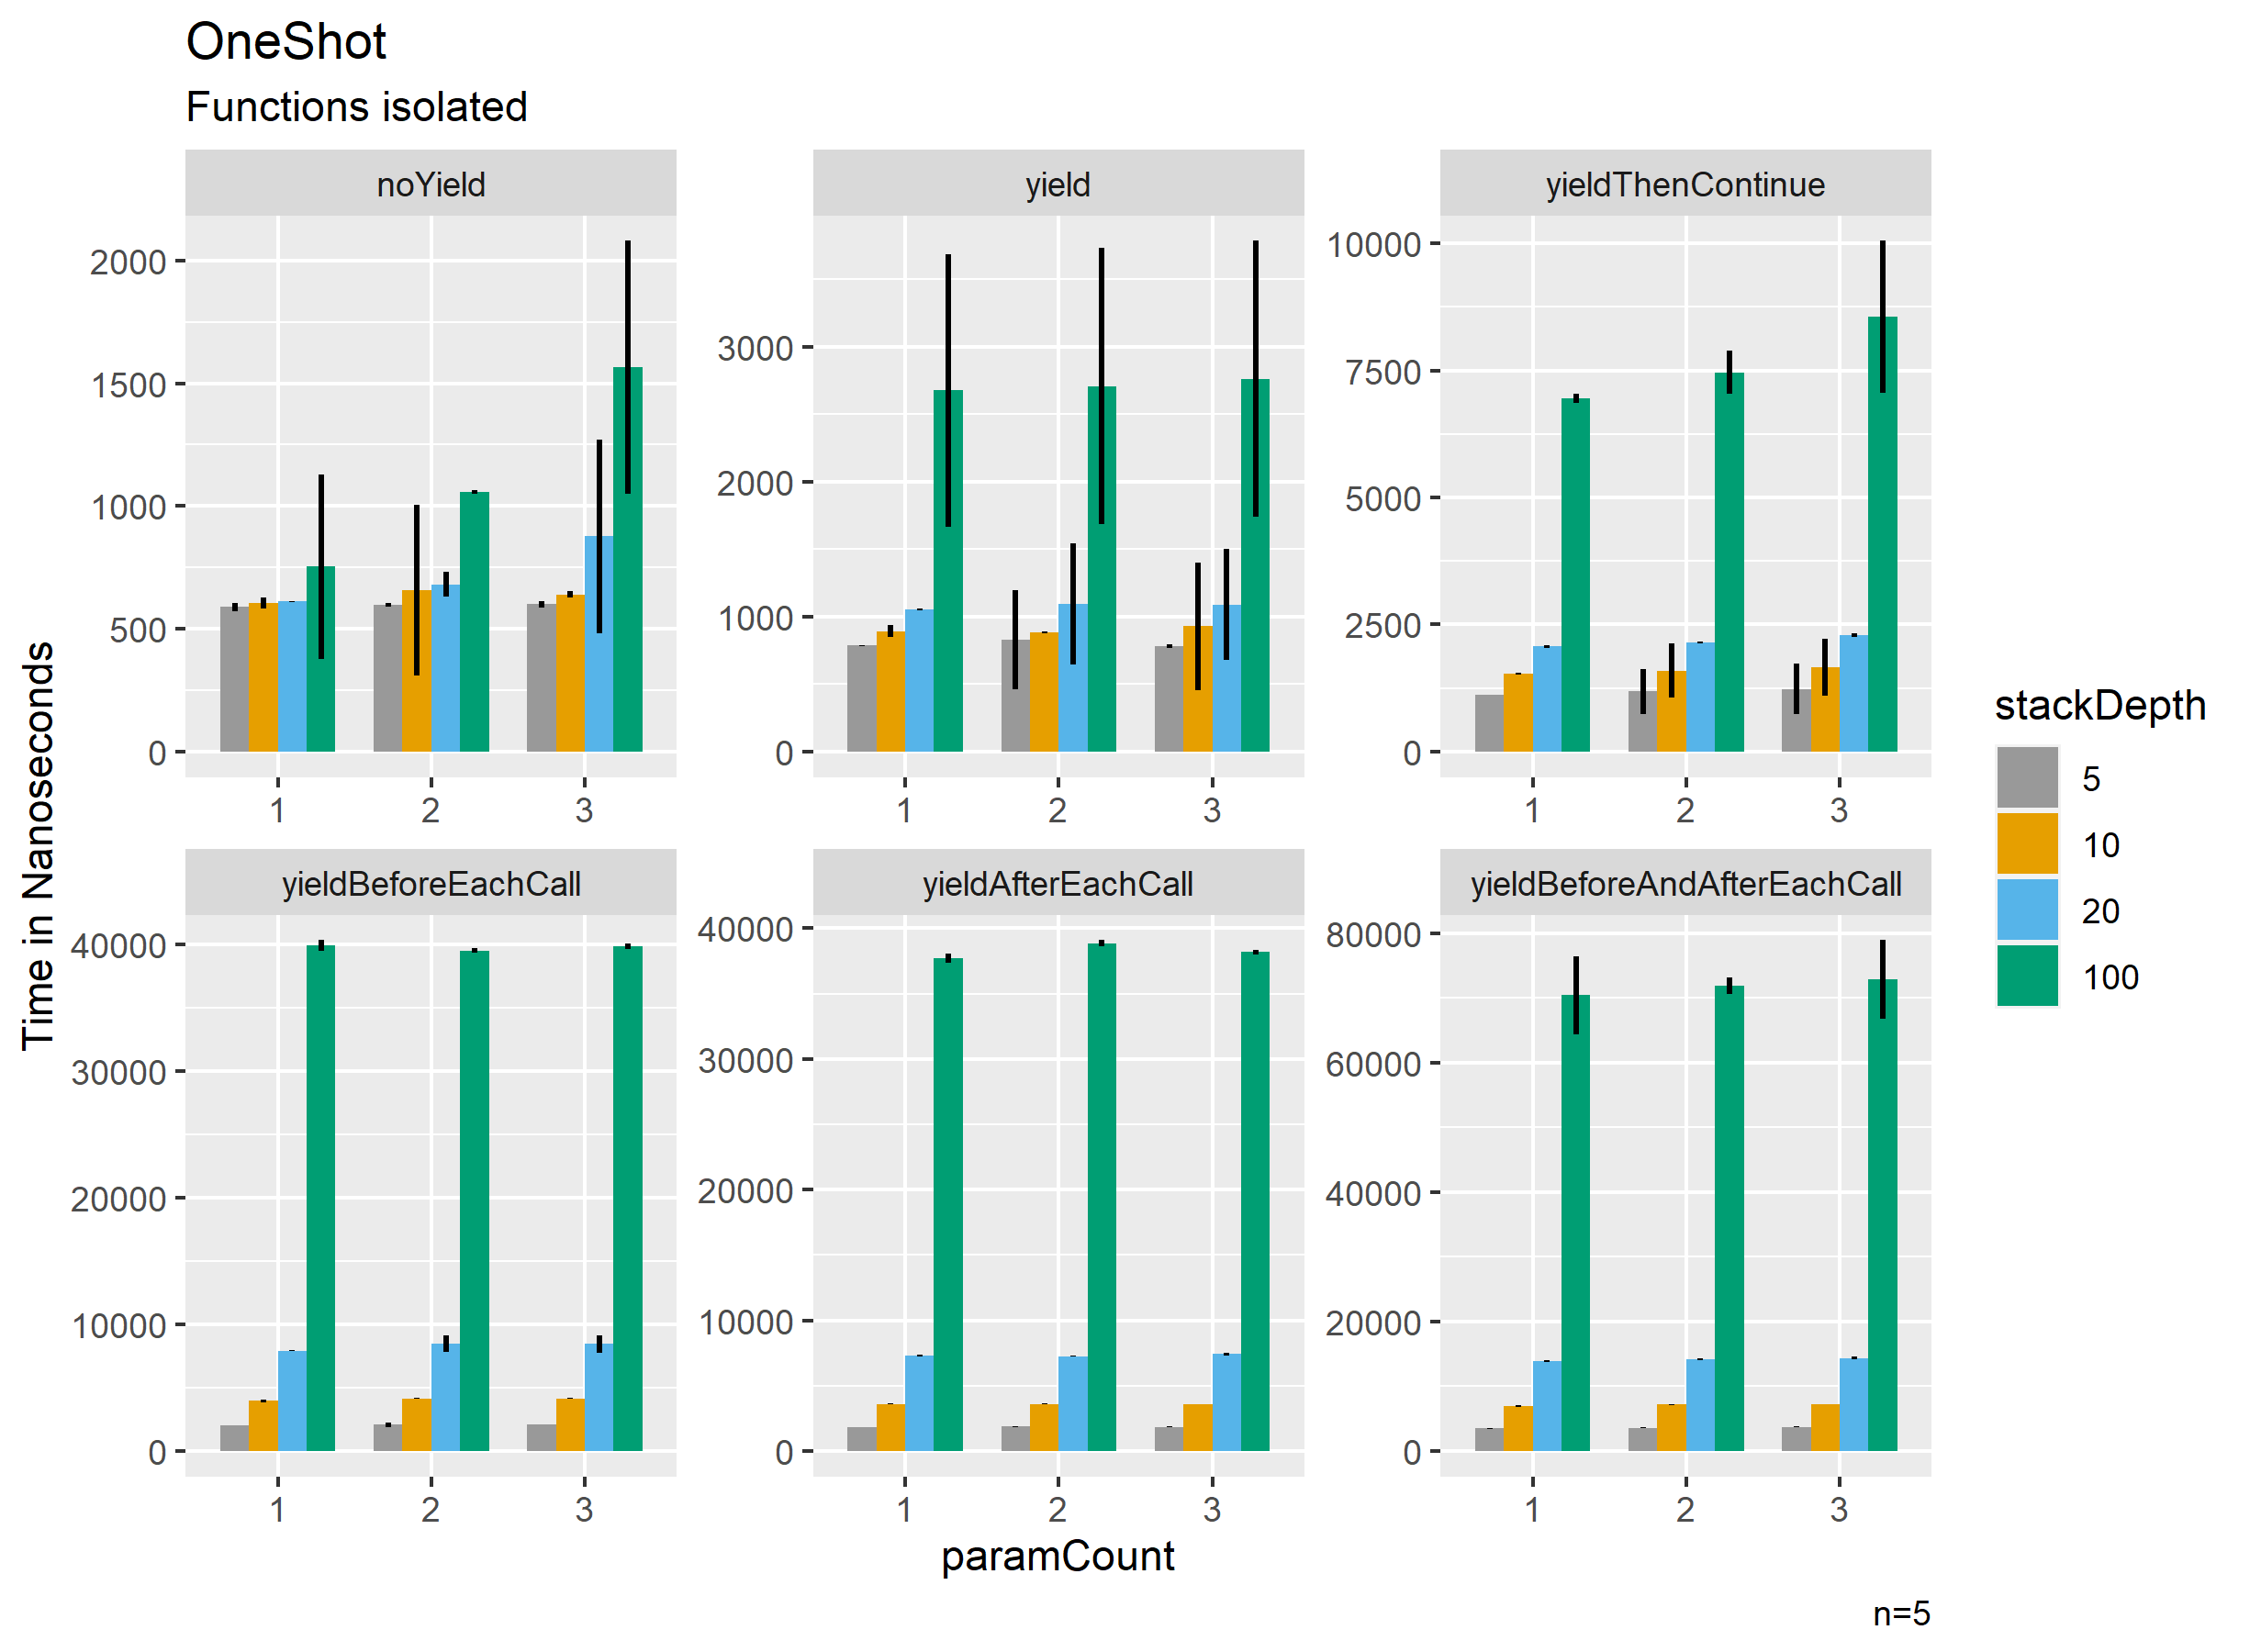
\includegraphics[width=1.0\linewidth]{img/jmh/OneShot.png}
  \end{subfigure}
  \caption{OneShot}
\end{figure}

One can also look at the individual functions in an isolated matter. One can immediately see that an increase in stack depth results in an increase in time. An increase in parameter count also seems to impact the time it takes to finish the task. One can observe it at a stack depth of 100.


\begin{figure}[H]
  \centering
  \begin{subfigure}[b]{1.0\textwidth}
    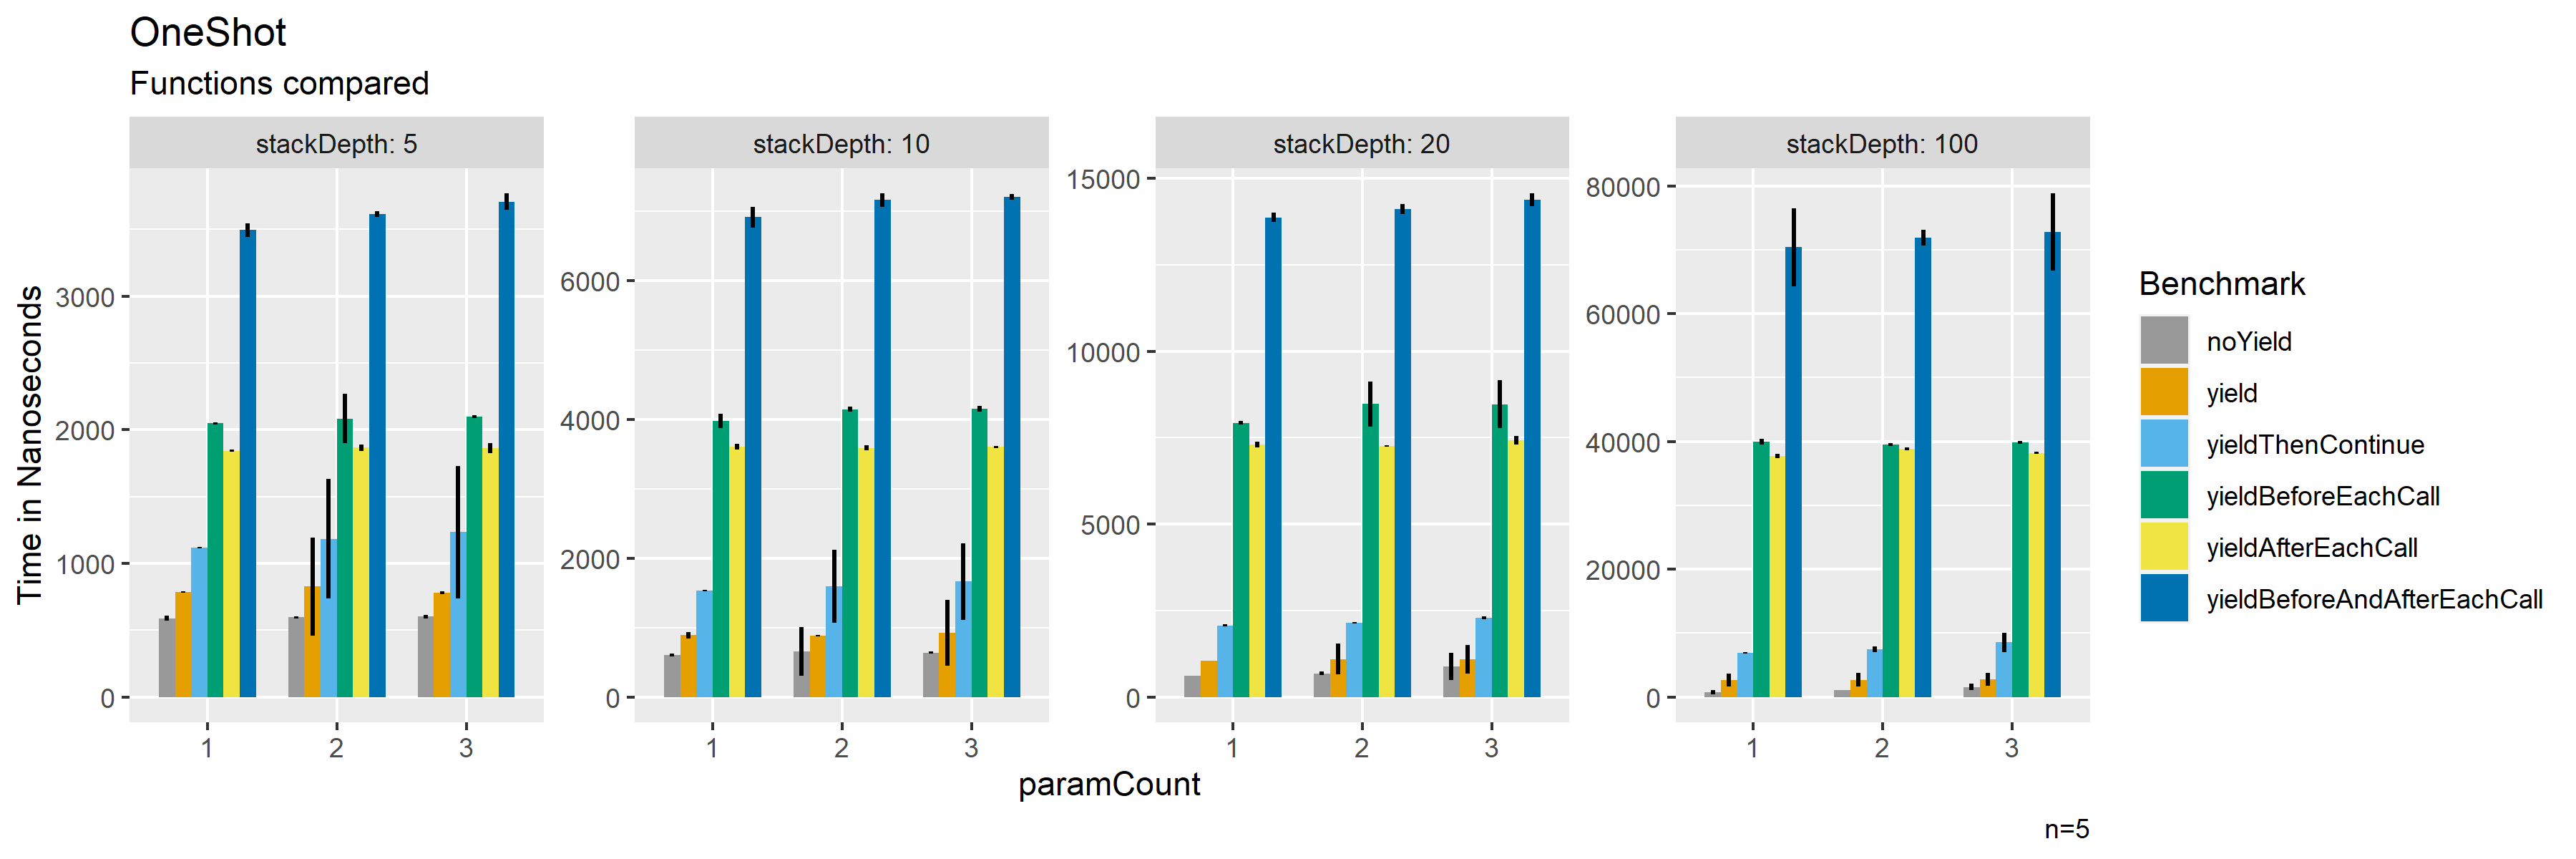
\includegraphics[width=1.0\linewidth]{img/jmh/OneShot2.png}
  \end{subfigure}
  \caption{OneShot}
\end{figure}





\subsection{Oscillation}
Here the continuation oscillates between a minimum and a maximum stack depth. It freezes at the maximum and continues afterwards.
One expectation here was that an increase in repetitions increases the time it takes to complete the task. This expectation has proven to be true. Another expectation was, that the bigger the difference from the minimal depth to the maximum depth is, the more time it would take to finish the task. This has also proven to be true.

\begin{figure}[H]
  \centering
  \begin{subfigure}[b]{1.0\textwidth}
    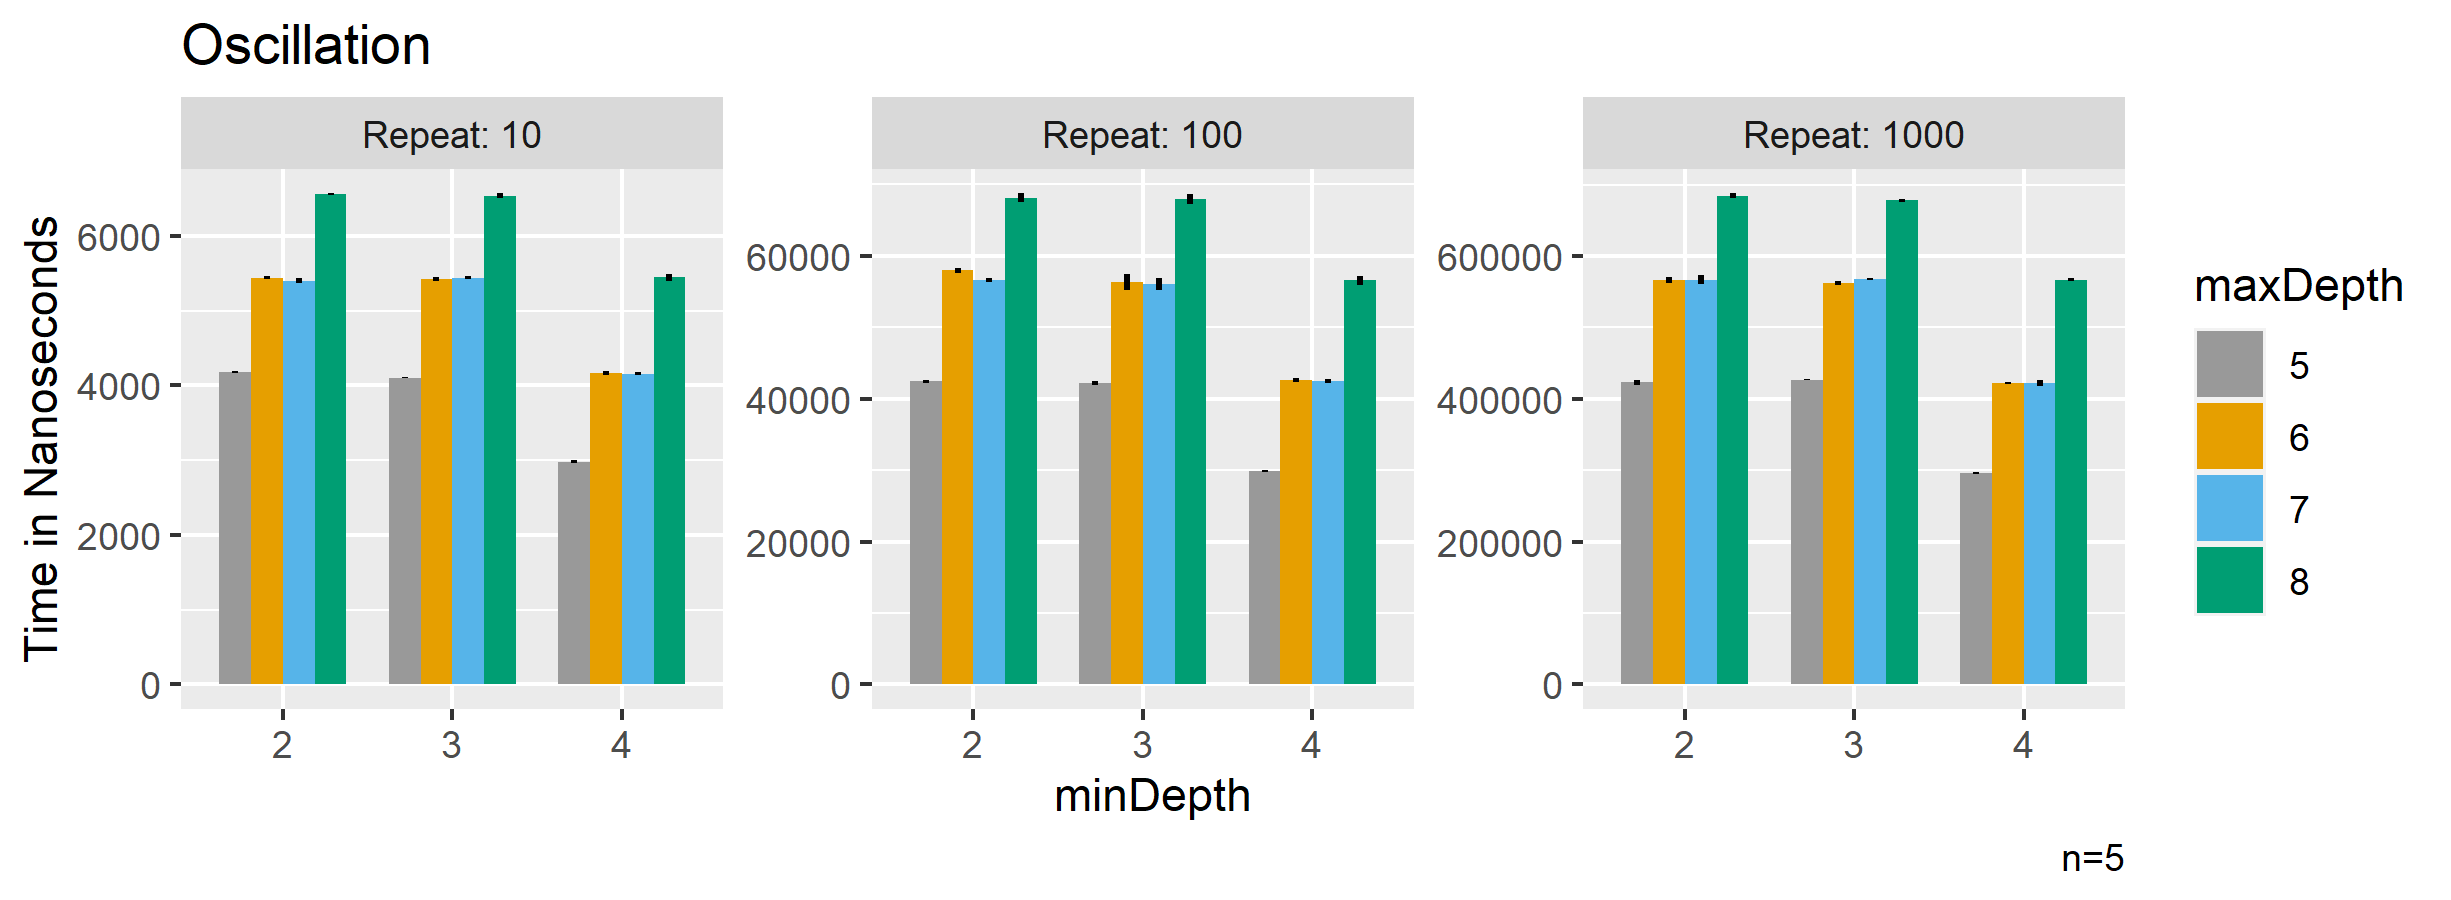
\includegraphics[width=1.0\linewidth]{img/jmh/Oscillation.png}
  \end{subfigure}
  \caption{Oscillation}
\end{figure}




\section{Footprint \& Performance}

\myparagraph{Experimental Setup}
Three Java classes are used in this experiment: EchoServerThread, EchoServerVThread, and Responder.
EchoServerThread and EchoServerVThread are almost identical. They both start a server that listens for requests on port 5566. Once a request is made, they start a separate thread, which runs the Responder class. Then they will continue to listen for further requests. The difference between the two classes is, that the EchoServerThread class utilizes kernel threads, while the EchoServerVThread class uses virtual threads. The Responder class sends a valid HTTP 1.1 header. Then it will echo the request it received.
\\
\\
Requests will be made using ApacheBench. All requests will be made with a concurrency of 100. Instead of running ApacheBench once with for example 1.000.000 requests, a shell script will be used. The shell script will then instead call ApacheBench 100 times in a row, with each run making 10.000 requests. This is done to remove ApacheBench as a potential bottleneck since it might not be fit to run 1.000.000 requests in a single process.
\\
\\
There will be two different kinds of measurement series:
\\
The first one is being recorded with VisualVM.
\\
The second one is recorded with JProfiler.
\\
There are multiple reasons for that. First off all a profiler might influence the measurements. Running similar tests with different profilers should improve the accuracy of the results. Also exporting the data is not possible using VisualVM. JProfiler allows one to export all measurements and model them as one wants to.

\myparagraph{Observed Values}
Heap size using VisualVM and JProfiler.
\\
Time to finish all requests using ApacheBench.


\subsection{Results - Profiler: VisualVM}
Virtual threads in orange and kernel threads in blue.
\\
\\
Looking at the scatter plots, one can immediately see that the virtual threads seem to not only perform better but also much more consistent than the kernel threads. When trying to model the results with linear regression, the first impression is further verified: The graph trying to model the virtual thread results is very precise. The margin for error is very small. On the other hand, the graph trying to model the kernel threads has a much bigger margin for error. This proves to be true in all 3 measurement series.

\begin{figure}[H]
  \centering
  \begin{subfigure}[b]{1.0\textwidth}
    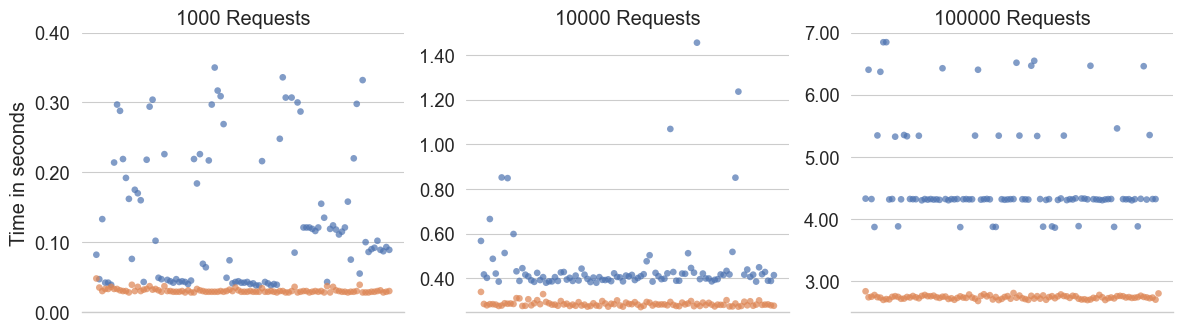
\includegraphics[width=1.0\linewidth]{img/footprint/scatter-100.png}
  \end{subfigure}
  \par\medskip % force a bit of vertical whitespace
  \begin{subfigure}[b]{1.0\textwidth}
    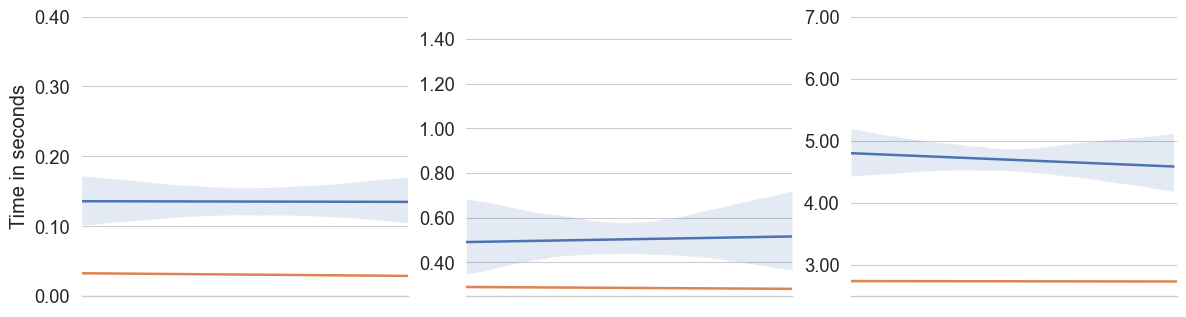
\includegraphics[width=1.0\linewidth]{img/footprint/linres-100.png}
  \end{subfigure}
  \caption{Time - Scatter \& Linear Regression - n=100 - VisualVM}
\end{figure}

Modeling the same results using boxplots allows one to take a closer look at the details. The 1000 requests series using virtual threads has a median of 30ms. The first and the third quartile are each 1ms above and below the median. Therefore 50\% of all the runs were completed between 29ms and 31ms. The 1000 requests series using kernel threads has a median around 100ms. The first quartile is slightly below 50ms and the third quartile is slightly above 200ms. That results in a spread of more than 150ms in the 50\% box.
\\
\\
The 10.000 requests series is more balanced: The 50\% box of the virtual threads series spans from 279ms to 289ms, resulting in a span of 10ms. The median is at 284ms. The 50\% box of the kernel threads series spans from 395ms to 430ms, resulting in a span of 35ms. The median is at 415ms. Any run that took longer than 480ms was considered an outlier for the kernel thread series and was not plotted. There are 10 such outliers.
\\
\\
In the 100.000 requests series, the 50\% box of the virtual threads run is slightly bigger than 25ms. The 50\% box of the kernel threads is slightly smaller than 20ms. Therefore this is the first series, in which the 50\% box spans a smaller range for the kernel threads. When one looks at the corresponding scatter plot, one can see, that there are more than 20 out of 100 runs, in which kernel threads needed more than 5 seconds to finish a run. Also, there are around 10 more runs, which were finished in less than 4 seconds. These 30 runs were considered outliers. No such outliers can be observed in the virtual thread series. Therefore, virtual threads perform more consistently once again.

\begin{figure}[H]
  \centering
  \begin{subfigure}[b]{1.0\textwidth}
    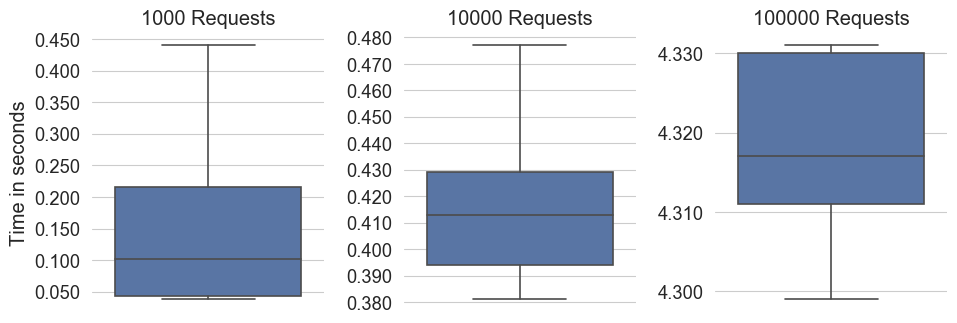
\includegraphics[width=1.0\linewidth]{img/footprint/boxplots-t-100.png}
  \end{subfigure}
  \par\medskip % force a bit of vertical whitespace
  \begin{subfigure}[b]{1.0\textwidth}
    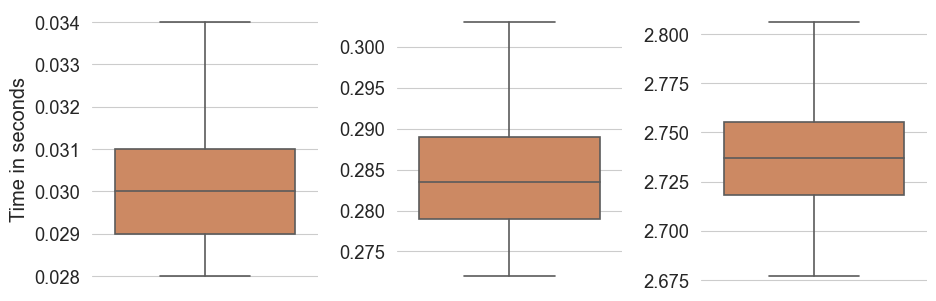
\includegraphics[width=1.0\linewidth]{img/footprint/boxplots-vt-100.png}
  \end{subfigure}
  \caption{Time - Boxplot - n=100 - VisualVM}
\end{figure}




\pagebreak
\subsection{Results - Profiler: JProfiler}
Virtual threads in orange and kernel threads in blue.
\\
\\
In the previous chapter the series with 1000 requests per run stuck out. Kernel threads performed especially more inconsistent in that series. Therefore the same experiment was run again here. Additionally, the number of runs was increased from 100 to 1000.

\begin{figure}[H]
  \centering
  \begin{subfigure}[b]{0.45\textwidth}
    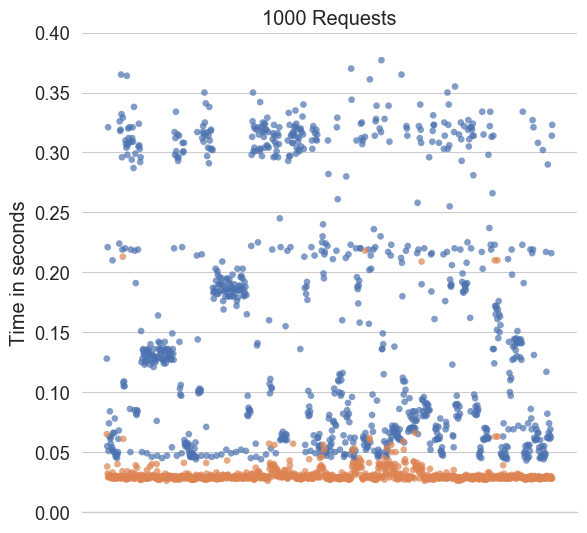
\includegraphics[width=1.0\linewidth]{img/footprint/scatter-1000.png}
  \end{subfigure}
  \begin{subfigure}[b]{0.45\textwidth}
    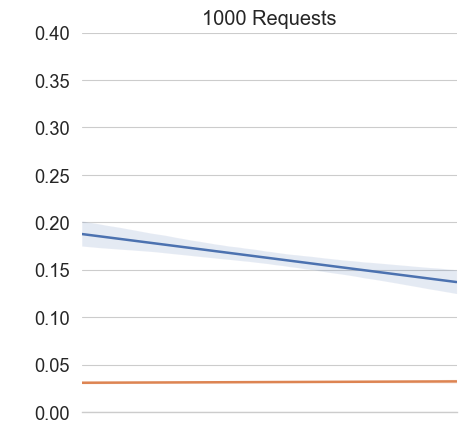
\includegraphics[width=1.0\linewidth]{img/footprint/linres-1000.png}
  \end{subfigure}
  \caption{Time - Scatter \& Linear Regression - n=1000 - JProfiler}
\end{figure}

Looking at the boxplots one can see, that the virtual threads performed similarly to before. The median is at 29ms, the 50\% box spans from 28ms to 30ms. The median of the kernel thread series is slightly higher than before. The 50\% box spans a range that is bigger than 100ms.

\begin{figure}[H]
  \centering
  \begin{subfigure}[b]{0.45\textwidth}
    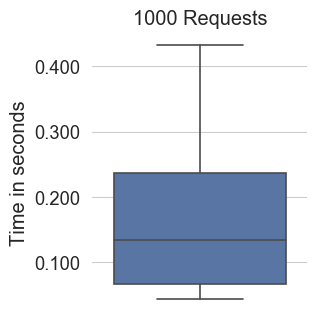
\includegraphics[width=1.0\linewidth]{img/footprint/boxplots-t-1000.png}
  \end{subfigure}
  \begin{subfigure}[b]{0.45\textwidth}
    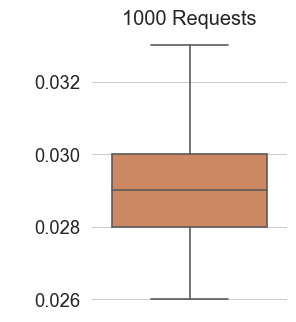
\includegraphics[width=1.0\linewidth]{img/footprint/boxplots-vt-1000.png}
  \end{subfigure}
  \caption{Time - Boxplot - n=1000 - JProfiler}
\end{figure}


Additionally, the heap usage is monitored this time around. Virtual threads use less heap space. They also are more consistent in their heap usage.


\begin{figure}[H]
  \centering
  \begin{subfigure}[b]{0.45\textwidth}
    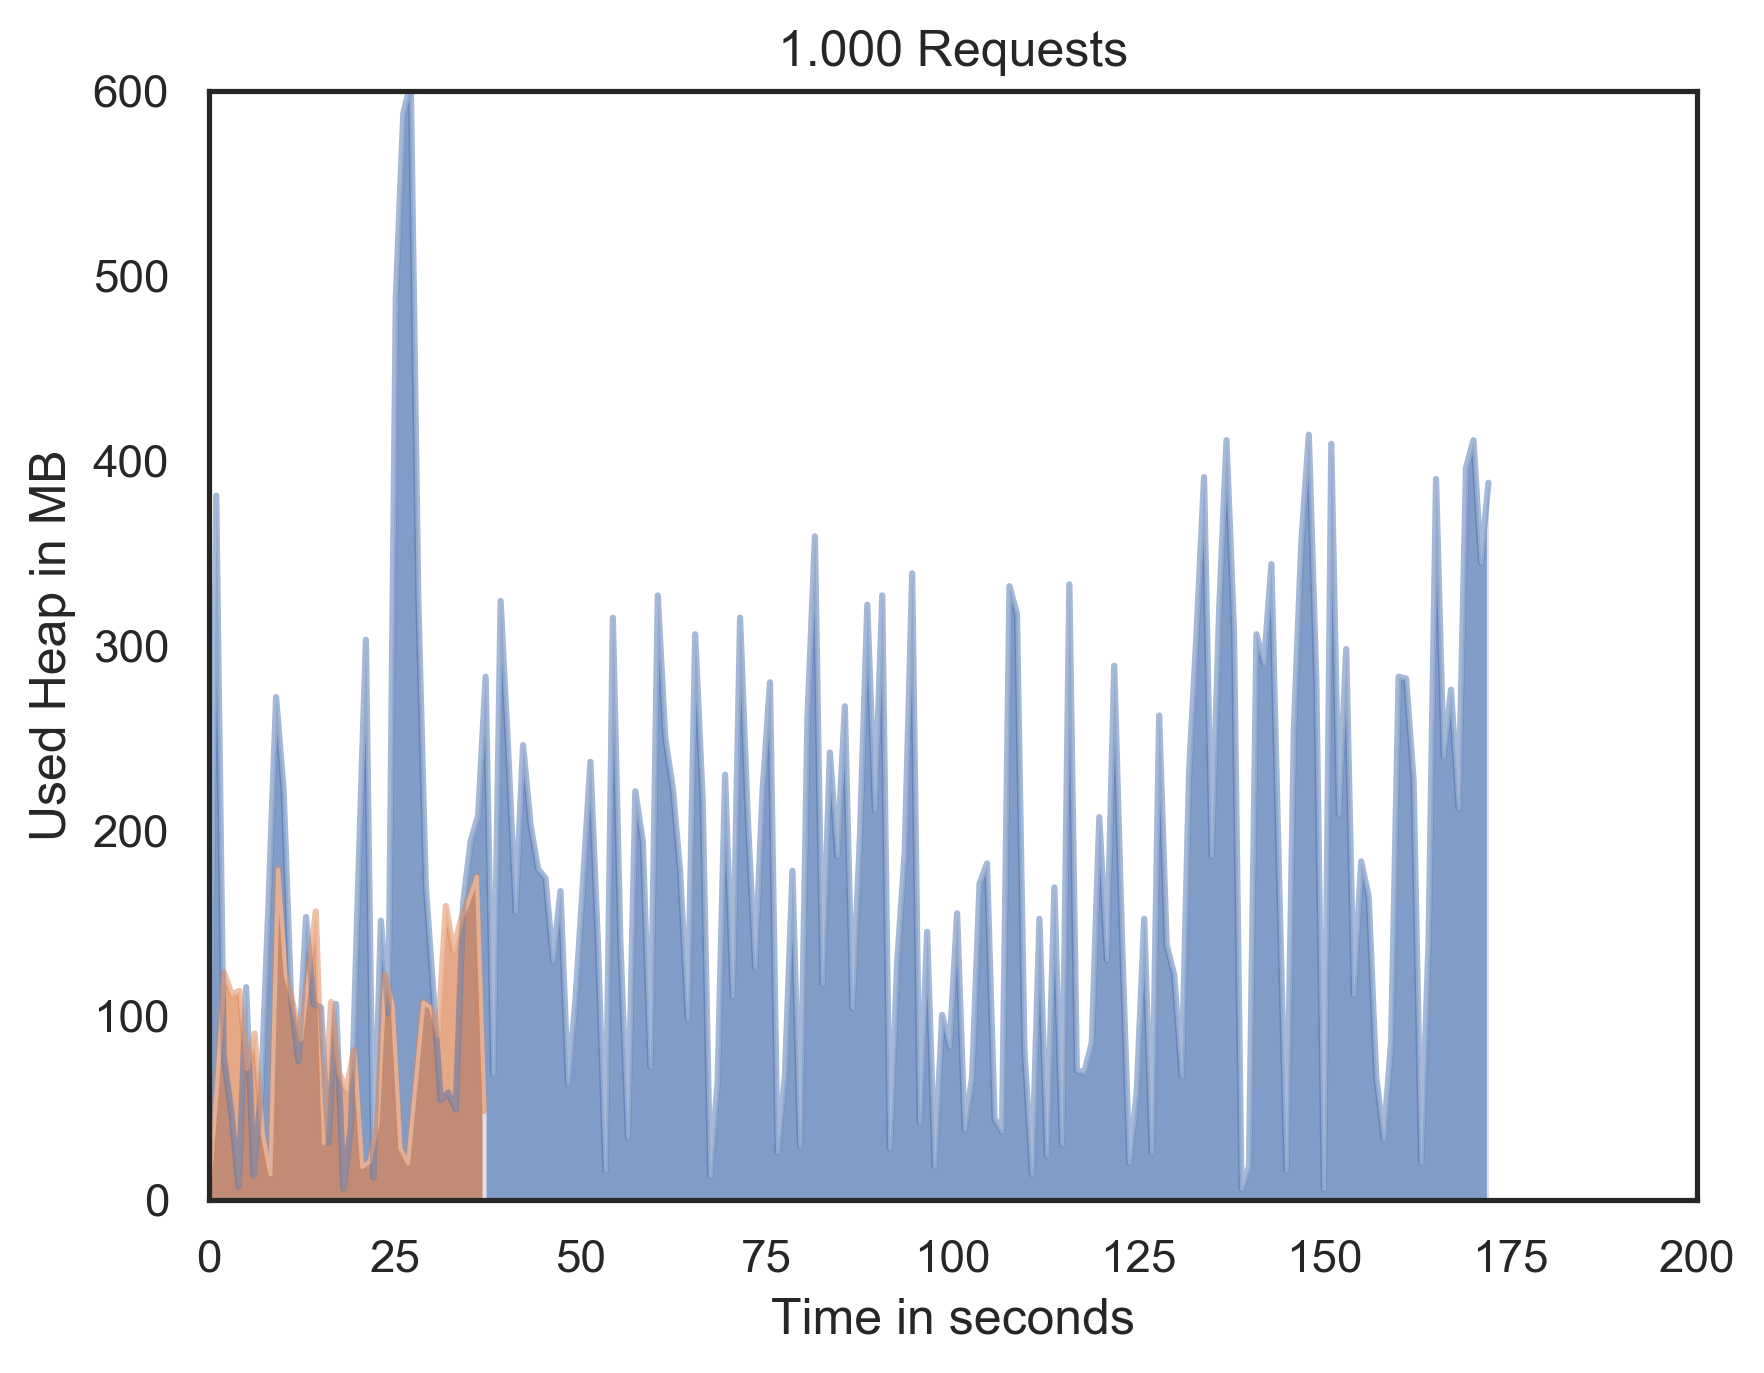
\includegraphics[width=1.0\linewidth]{img/footprint/heap_1000_line.png}
  \end{subfigure}
  \begin{subfigure}[b]{0.3\textwidth}
    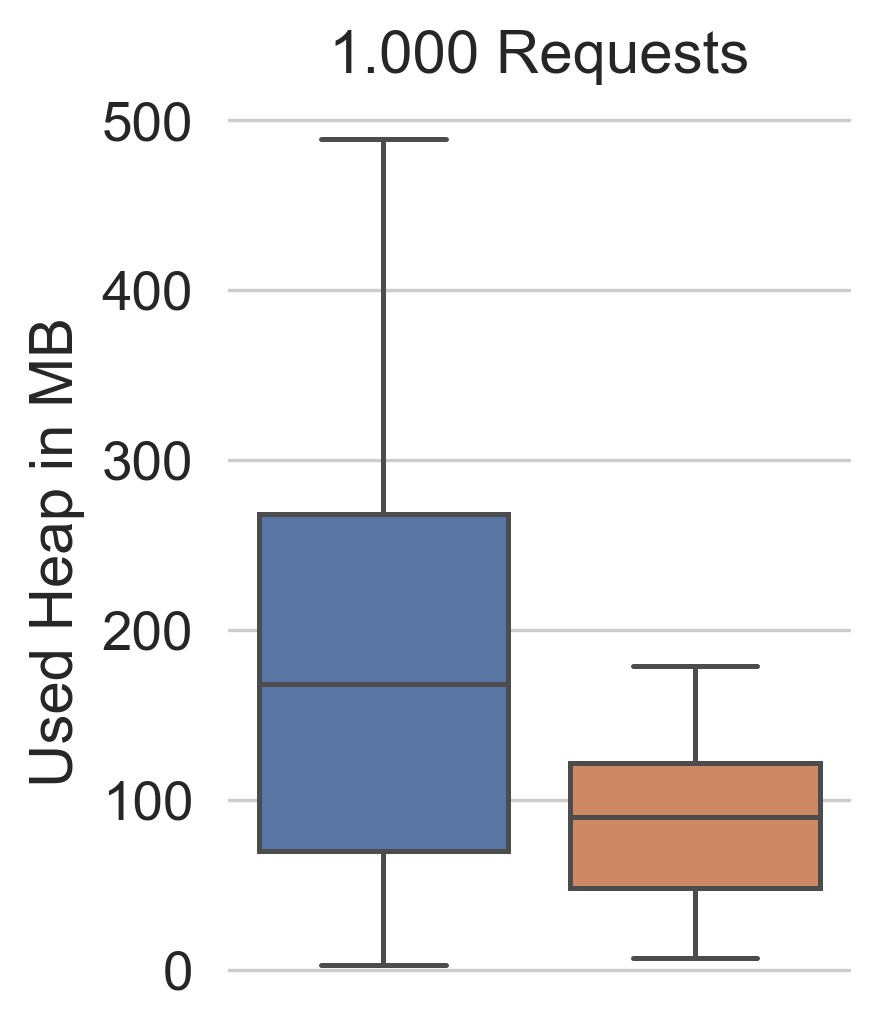
\includegraphics[width=1.0\linewidth]{img/footprint/heap_1000_box.png}
  \end{subfigure}
  \caption{Heap Usage - n=1000 - JProfiler}
\end{figure}

\pagebreak
The following series measures 10.000 requests, ran 500 times. Originally this series was intended to be ran 1000 times. That was not possible, because the Linux kernel consistently killed the EchoServerThread process at around 600 runs.
\\
\\
Virtual threads perform better and more consistent once again. Most runs were finished faster than 300ms. Looking at the kernel threads, the majority of runs were finished around 500ms. There also is a significant minority of runs finishing around 800-900ms.
\begin{figure}[H]
  \centering
  \begin{subfigure}[b]{0.45\textwidth}
    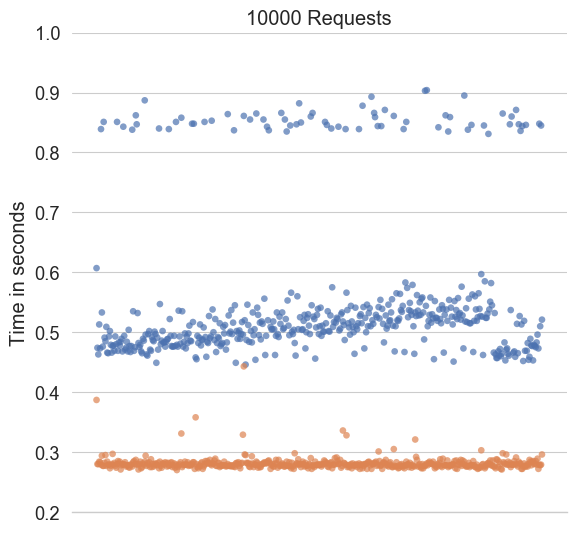
\includegraphics[width=1.0\linewidth]{img/footprint/scatter-500.png}
  \end{subfigure}
  \begin{subfigure}[b]{0.45\textwidth}
    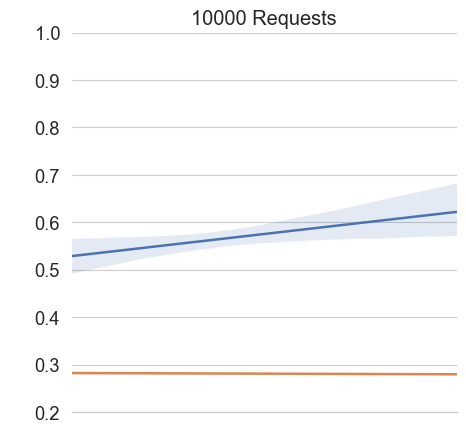
\includegraphics[width=1.0\linewidth]{img/footprint/linres-500.png}
  \end{subfigure}
  \caption{Time - Scatter \& Linear Regression - n=500- JProfiler}
\end{figure}

The median of the virtual thread series is 278ms. The median of the kernel thread series is 513ms. That is a decrease of more than 40\%. Also, the virtual thread 50\% box spans an area of 5ms here, while the kernel threads span an area of around 50ms.

\begin{figure}[H]
  \centering
  \begin{subfigure}[b]{0.45\textwidth}
    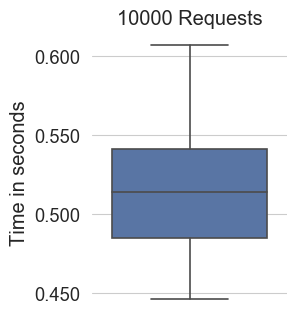
\includegraphics[width=1.0\linewidth]{img/footprint/boxplots-t-500.png}
  \end{subfigure}
  \begin{subfigure}[b]{0.45\textwidth}
    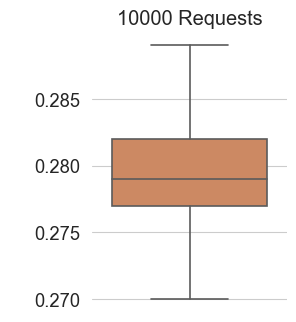
\includegraphics[width=1.0\linewidth]{img/footprint/boxplots-vt-500.png}
  \end{subfigure}
  \caption{Time - Boxplot - n=500 - JProfiler}
\end{figure}

Once again, the heap usage is significantly higher using kernel threads. The median of the kernel thread series is 200MB, while the virtual thread series has a median of 100MB. 

\begin{figure}[H]
  \centering
  \begin{subfigure}[b]{0.45\textwidth}
    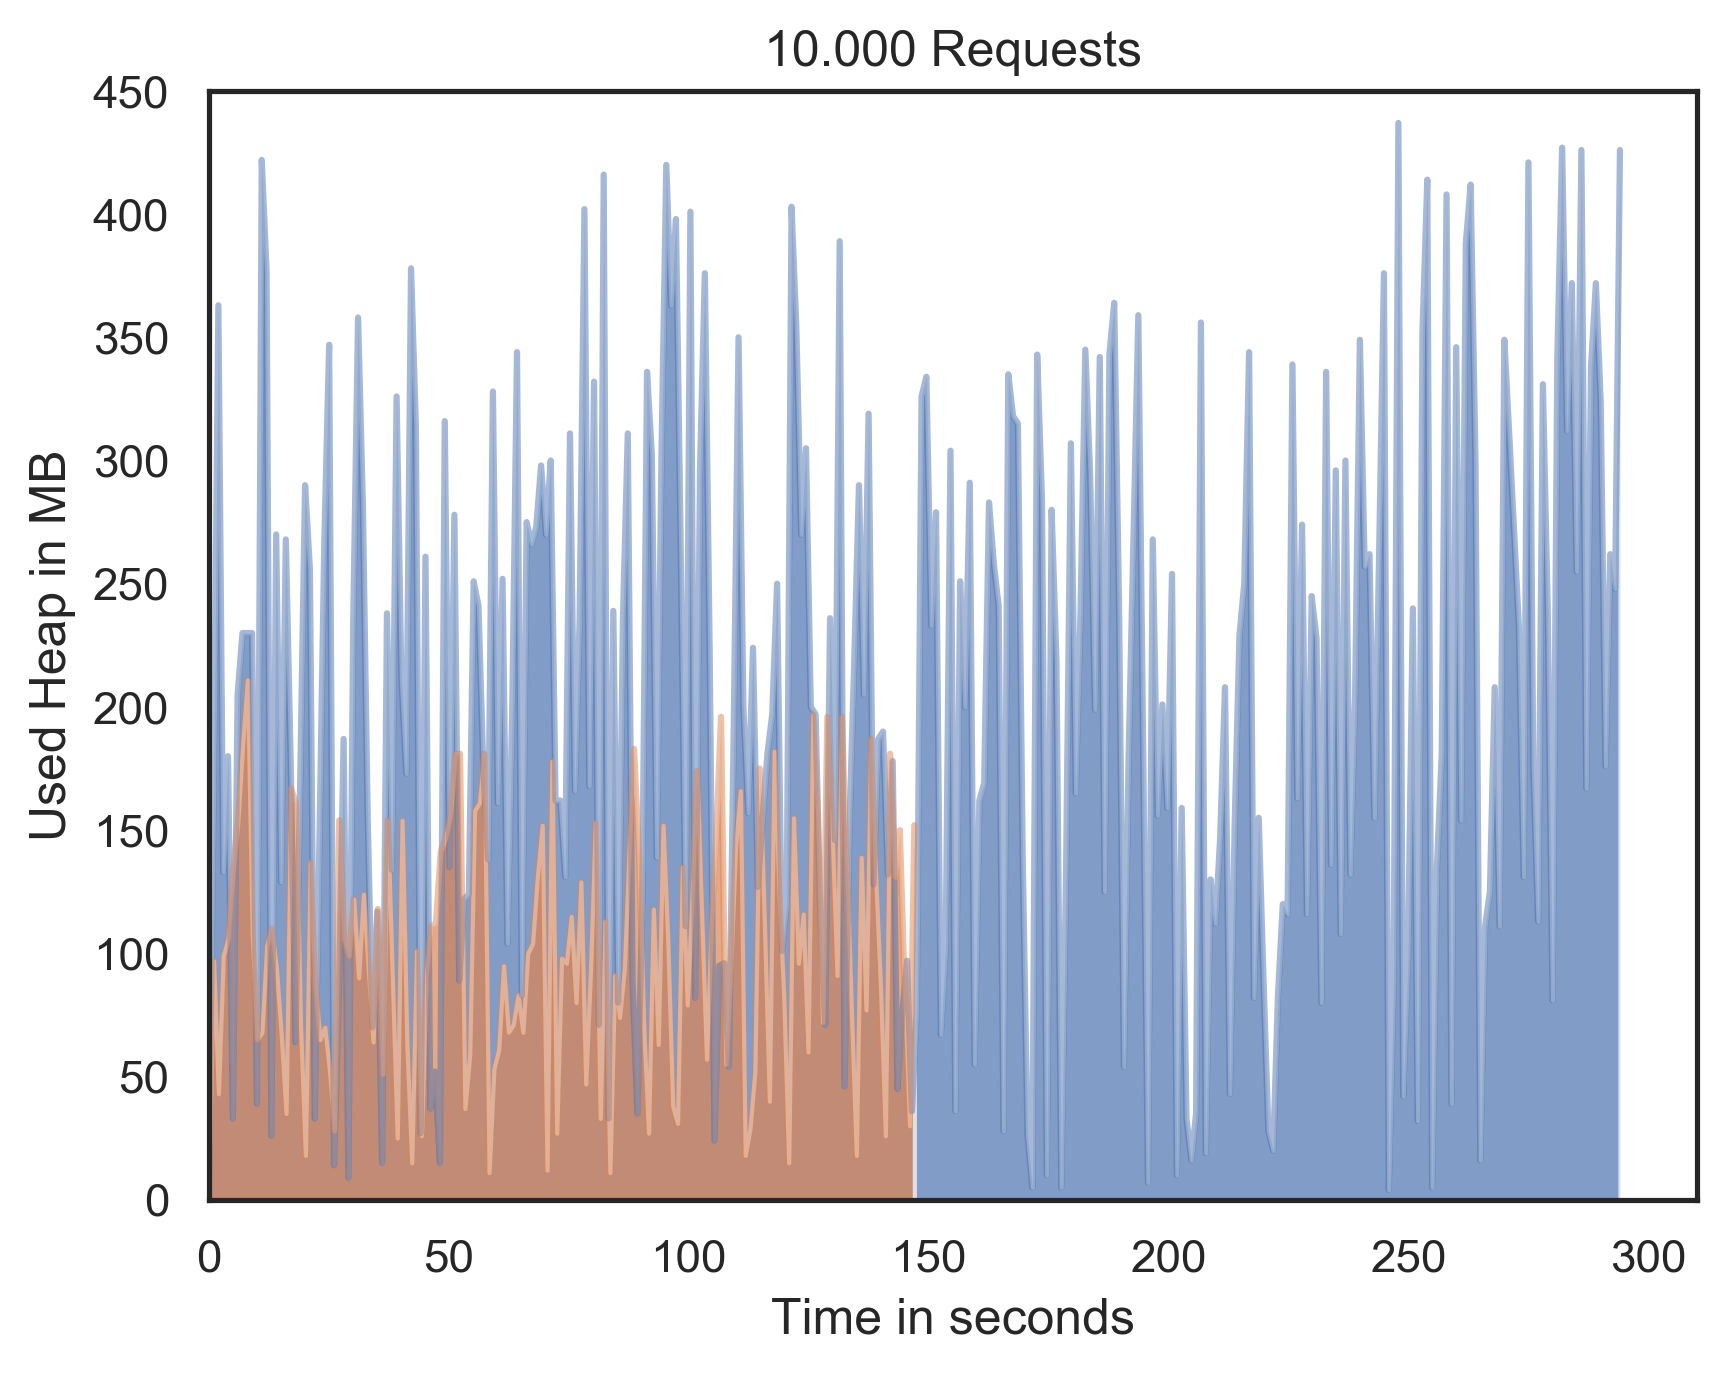
\includegraphics[width=1.0\linewidth]{img/footprint/heap_500_line.png}
  \end{subfigure}
  \begin{subfigure}[b]{0.3\textwidth}
    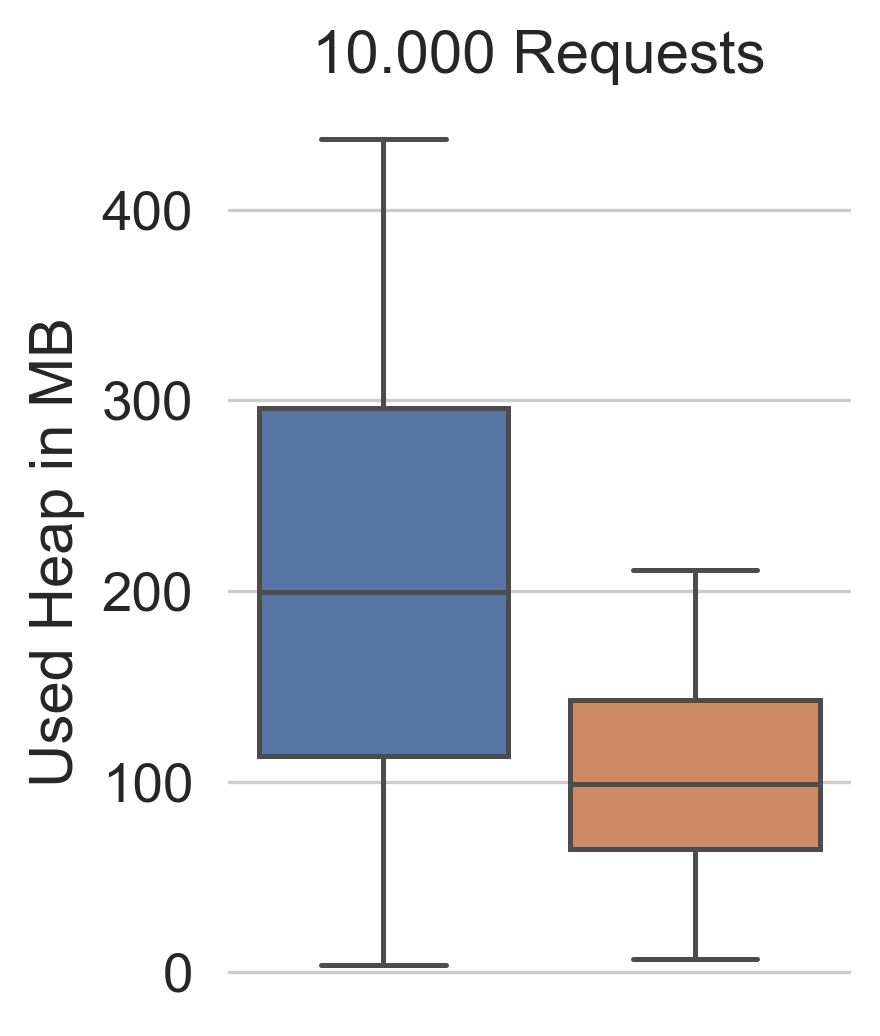
\includegraphics[width=1.0\linewidth]{img/footprint/heap_500_box.png}
  \end{subfigure}
  \caption{Heap Usage - n=500 - JProfiler}
\end{figure}




\section{Evaluation of the implementation Loom}

Wrapping up the observations from the experiments:
\begin{itemize}
  \item Virtual threads are faster.
  \item Virtual threads perform more consistently.
  \item Virtual threads require less heap space for the same task.
\end{itemize}

The transition from kernel to virtual threads is, or at least envisioned to be, effortless. A free 33\% increase in performance and a 50\% decrease in footprint is not only something existing pieces of software written in Java will appreciate but also a strong argument for newer projects to use Java. Therefore, it is very much in Oracle's interest, that the project will successfully be finished as soon as possible. 
\\
\\
Also, project Loom is already part of the newer OpenJDK releases. Old APIs, that were not compatible with virtual threads, are already being reworked. As an example, the network API has already been changed and supports virtual threads now.
\\
\\
With all these observations in mind, it is highly unlikely, that the project won't be finished. It will provide a significant performance increase to the Java ecosystem.
    \chapter{Conclusion}
This thesis consists of two major parts.
\\
\\
The first one is the code analysis. Analyzing a work in progress is a time-intensive task. Documentation existed almost exclusively in Java comments here and there in the code. The only way to deal with that problem was to simply invest more time in the analysis. That worked up until intrinsics appeared. There is information regarding HotSpot intrinsics on the internet, but those are very general. For specific information regarding intrinsics in project Loom, the solution was to contact the maintainers directly. Once that information was gained, it was obvious, that the intrinsics of project Loom are beyond the scope of this thesis.
\\
\\
The second one is the experiment. There were two experiments. The first one consisted of running the JMH benchmarks project Loom uses themselves. To understand them, one had to read the documentation of the JMH framework thoroughly. Afterwards, one could simply run them and plot the results. Project Loom is still doing a lot of tests in regards to performance. Future works regarding project Loom might be able to pick up these results and compare them to the results of newer versions.
\\
The second experiment was intended to simulate a big-data-framework. Resources were limited both hardware and software-wise. Originally, the experiment was intended to be run on the cluster of the Operating Systems Research group. Due to COVID-19, the experiment had to be run on personal hardware instead. Also, because the thesis was already very time intensive in regards to the code analysis, there wasn't infinite time to create a very complex piece of software. Despite that, the software still had to be realistic. Therefore the decision was made, to use an EchoServer. The EchoServer combined elements of networking and multithreading, without demanding too much time to code it.
\\
Finally, benchmarks could be run. Once again, time was a limiting factor here. For example, one benchmark, that did not end up being included in the thesis, had the following parameters: 1.000.000 requests and n=100. Running a single set of 1.000.000 requests using kernel threads took up to 1minute. So just running the kernel thread benchmark took around 1,5h. Often, the benchmark would crash during that too. So the benchmark had to be ran multiple times to ensure, that the results are accurate. That ended up being too time intensive. Therefore, the decision was made, to rather run small benchmarks. If one of these benchmarks failed, the damage was much smaller. 

\end{abschlussarbeit}
\end{document}

